% ===========================================================================
%  SWC 2026 Problem C -- skeleton with slot-only numbers.
%  Every numeral in the body comes from slots.tex (generated by
%  code/fill_numbers.py out of data/*.json). Nothing here is typed by hand.
%  Compile: see snippets/reproduce.ps1 (xelatex, two passes).
% ===========================================================================
\documentclass{swmcmthesis}
\usepackage{algorithm}
\usepackage{algpseudocode}
\usepackage{float}
\usepackage{longtable}
\usepackage{indentfirst}
\usepackage{microtype}
\microtypesetup{protrusion=false}
\lstset{basicstyle=\small\ttfamily,breaklines=true,columns=fullflexible,keepspaces=true}
\usepackage{array}
\usepackage{titlesec}
% numerals-ok: begin
\titleformat{\section}{\normalfont\large\bfseries}{\thesection}{0.7em}{}[\vspace{2pt}{\color{gray!45}\hrule height 0.5pt}]
\titlespacing*{\section}{0pt}{11pt plus 2pt minus 2pt}{6pt}
\titleformat{\subsection}{\normalfont\normalsize\bfseries}{\thesubsection}{0.6em}{}
\titlespacing*{\subsection}{0pt}{10pt plus 2pt minus 2pt}{4pt}
\titleformat{\subsubsection}{\normalfont\normalsize\itshape}{\thesubsubsection}{0.6em}{}
\titlespacing*{\subsubsection}{0pt}{8pt plus 2pt minus 1pt}{3pt}
\usepackage[hidelinks]{hyperref}
% numerals-ok: end
% numerals-ok: begin
\renewcommand{\arraystretch}{0.92}
% numerals-ok: end

% ---- typographic baseline: one uniform first-line indent, no ragged last pages ----
% numerals-ok: begin
\setlength{\parindent}{2em}
\setlength{\parskip}{0pt}
\widowpenalty=10000
\clubpenalty=10000
\raggedbottom
% numerals-ok: end
% numerals-ok: begin
\captionsetup[figure]{font=small,labelfont=bf,textfont=normalfont,labelformat=simple,labelsep=period,skip=6pt,format=hang}
\captionsetup[table]{font=small,labelfont=bf,textfont=normalfont,labelformat=simple,labelsep=period,skip=4pt,format=hang,position=above}
\setlength{\abovecaptionskip}{9pt}
\setlength{\belowcaptionskip}{5pt}
% numerals-ok: end

% slots.tex -- GENERATED by code/fill_numbers.py. Do not edit by hand.
% Every number printed in main.tex comes from this file.
% [spec] state-layer rule a_grasp
\newcommand{\slotAGrasp}{0.15}
% [spec] P3 mapping set
\newcommand{\slotAlphaHigh}{1.5}
% [spec] P3 mapping set
\newcommand{\slotAlphaLow}{0.75}
% [spec] P3 nominal mapping
\newcommand{\slotAlphaNom}{1}
% [spec] P3 minimum reservation
\newcommand{\slotBMin}{0.2}
% [spec] P3 mapping set
\newcommand{\slotBetaHigh}{1}
% [spec] P3 mapping set
\newcommand{\slotBetaLow}{0}
% [spec] P3 nominal mapping
\newcommand{\slotBetaNom}{0.5}
% [spec] layout
\newcommand{\slotBibWidth}{99}
% [spec] P3 budget S1
\newcommand{\slotBudgetSOne}{32}
% [spec] P3 budget S3
\newcommand{\slotBudgetSThree}{40}
% [spec] P3 budget S2
\newcommand{\slotBudgetSTwo}{34}
% [spec] reporting convention: paired 95% confidence interval
\newcommand{\slotCILevel}{95}
% [spec] case label S1
\newcommand{\slotCaseOne}{1}
% [spec] case label S3
\newcommand{\slotCaseThree}{3}
% [spec] case label S2
\newcommand{\slotCaseTwo}{2}
% [spec] P3 travel change-over time
\newcommand{\slotChangeOver}{0.5}
% [spec] P2 nominal conformal level
\newcommand{\slotConfLevel}{90}
% [spec] P3 execution cost coefficient of b
\newcommand{\slotCostB}{0.1}
% [spec] P3 execution cost constant
\newcommand{\slotCostBase}{2}
% [spec] P3 execution cost coefficient of D
\newcommand{\slotCostD}{0.2}
% [spec] P2 frozen context length
\newcommand{\slotCtx}{10}
% [spec] statement: EgoDemo
\newcommand{\slotDemoRecords}{31}
% [spec] statement: EgoDemo timestamps
\newcommand{\slotDemoTS}{16414}
% [spec] package audit: declared head-depth rate
\newcommand{\slotDepthFPS}{5}
% [spec] package audit: declared head-depth height
\newcommand{\slotDepthH}{240}
% [spec] package audit: declared head-depth width
\newcommand{\slotDepthW}{320}
% [spec] layout: display skip
\newcommand{\slotDisplayAbove}{4pt plus 2pt minus 2pt}
% [spec] layout: display skip
\newcommand{\slotDisplayBelow}{4pt plus 2pt minus 2pt}
% [spec] layout
\newcommand{\slotEmergStretch}{3em}
% [spec] statement / data: 30 Hz
\newcommand{\slotFPS}{30}
% [spec] layout
\newcommand{\slotFigW}{0.78\linewidth}
% [spec] layout
\newcommand{\slotFigWFull}{0.96\linewidth}
% [spec] layout
\newcommand{\slotFigWSmall}{0.66\linewidth}
% [spec] layout
\newcommand{\slotFigWSub}{0.43\linewidth}
% [spec] layout: float separation
\newcommand{\slotFloatIntSep}{4pt plus 1pt minus 1pt}
% [spec] layout: float separation
\newcommand{\slotFloatSep}{4pt plus 1pt minus 1pt}
% [spec] layout: float separation
\newcommand{\slotFloatTextSep}{6pt plus 1pt minus 1pt}
% [spec] frozen reliability fusion weight
\newcommand{\slotFusionWeight}{0.5}
% [spec] P3 horizon S1
\newcommand{\slotHSOne}{100}
% [spec] P3 horizon S3
\newcommand{\slotHSThree}{125}
% [spec] P3 horizon S2
\newcommand{\slotHSTwo}{100}
% [spec] layout
\newcommand{\slotHeadHeight}{20pt}
% [spec] P3 case S1
\newcommand{\slotJobsSOne}{8}
% [spec] P3 case S3
\newcommand{\slotJobsSThree}{16}
% [spec] P3 case S2
\newcommand{\slotJobsSTwo}{12}
% [spec] frozen BIC search range for the segment count
\newcommand{\slotKMax}{8}
% [spec] frozen BIC search range for the segment count
\newcommand{\slotKMin}{2}
% [spec] P3 review limit S1
\newcommand{\slotKSOne}{4}
% [spec] P3 review limit S3
\newcommand{\slotKSThree}{8}
% [spec] P3 review limit S2
\newcommand{\slotKSTwo}{6}
% [spec] frozen logistic regularisation, code/p1_model.py
\newcommand{\slotLogitC}{0.1}
% [spec] P2 frozen mask set
\newcommand{\slotMaskA}{0.2}
% [spec] P2 frozen mask set
\newcommand{\slotMaskB}{0.5}
% [spec] P2 frozen mask set
\newcommand{\slotMaskC}{1.0}
% [spec] P2 frozen mask set
\newcommand{\slotMaskD}{2.0}
% [spec] P3 action cap per trial
\newcommand{\slotMaxActions}{200}
% [spec] P3 reviews per job
\newcommand{\slotMaxReviewsPerJob}{2}
% [spec] P3 eligibility threshold
\newcommand{\slotMinEligibleDur}{1.2}
% [spec] referenced Data_Documentation files absent from the package
\newcommand{\slotMissingDocs}{5}
% [spec] P3 intervals of at least 1.2 s
\newcommand{\slotNEligible}{343}
% [spec] statement: 24 environments
\newcommand{\slotNEnv}{24}
% [spec] P3 attachment intervals
\newcommand{\slotNIntervals}{349}
% [spec] statement: 21 3D keypoints per hand
\newcommand{\slotNKeypoints}{21}
% [spec] statement: 69 records, 24 environments
\newcommand{\slotNRecords}{69}
% [spec] P3 official seed list
\newcommand{\slotNSeeds}{30}
% [spec] discrete state layer: reach/pick/place/transport/arrange
\newcommand{\slotNStages}{5}
% [spec] statement: 66,070 timestamps
\newcommand{\slotNTimestamps}{66070}
% [spec] package audit: video files
\newcommand{\slotNVideos}{184}
% [spec] P3 required mean weighted on-time rate
\newcommand{\slotOnTimeFloor}{0.50}
% [spec] P3 required mean weighted on-time rate, percent
\newcommand{\slotOnTimeFloorPct}{50}
% [spec] mapping-sensitivity grid: long service multiplier
\newcommand{\slotPCFAlphaHigh}{1.5}
% [spec] mapping-sensitivity grid: short service multiplier
\newcommand{\slotPCFAlphaLow}{0.75}
% [spec] nominal service multiplier
\newcommand{\slotPCFAlphaNom}{1.0}
% [spec] state-layer definition; the package ships no product annotations
\newcommand{\slotPProductStateVars}{grasp success and shelf occupancy}
% [spec] common_conditions.json: observation.delay_s (fixed by the protocol, not measured)
\newcommand{\slotPSchedDelayDistribution}{1.0}
% [spec] relative: p3_final_duration.json visual_a300 test MAE 2.5746 vs pose_old8 ridge 3.0920 (p3_visual_duration.json)
\newcommand{\slotPVisDurRel}{-16.7}
% [spec] p3_visual_schedule.json minus p3_stochastic_schedule.json, oracle S3, ceiling shift
\newcommand{\slotPVisOracleSThreeD}{+0.025}
% [spec] p3_visual_schedule.json minus p3_stochastic_schedule.json, slack_fusion S3, same 30 seeds
\newcommand{\slotPVisSchedSThreeD}{-0.009}
% [spec] p3_visual_schedule.json minus p3_stochastic_schedule.json, slack_fusion S2, same 30 seeds
\newcommand{\slotPVisSchedSTwoD}{+0.031}
% [spec] state-layer rule: palm-centre keypoints
\newcommand{\slotPalmKeypoints}{0, 5, 9, 13, 17}
% [spec] pre-declared P1 segmentation pass mark
\newcommand{\slotPassARI}{0.35}
% [spec] pre-declared P1 reliability pass mark
\newcommand{\slotPassAUC}{0.55}
% [spec] pre-declared P1 segmentation pass mark
\newcommand{\slotPassCountErr}{10}
% [spec] pre-declared P1 segmentation pass mark
\newcommand{\slotPassFOne}{0.45}
% [spec] P3 free prefix
\newcommand{\slotPrefixFree}{0.2}
% [spec] P3 second paid review prefix
\newcommand{\slotPrefixLong}{1.0}
% [spec] P3 first paid review prefix
\newcommand{\slotPrefixMid}{0.6}
% [spec] statement: EgoPro
\newcommand{\slotProRecords}{14}
% [spec] statement: EgoPro timestamps
\newcommand{\slotProTS}{17642}
% [spec] P2 reactive baseline threshold, cm
\newcommand{\slotReactiveCM}{5}
% [spec] frozen reservation residual quantile, percent
\newcommand{\slotReserveQ}{60}
% [spec] P3 review cost unit
\newcommand{\slotReviewCost}{1}
% [spec] P3 review scenario-second delay
\newcommand{\slotReviewDelay}{1}
% [spec] frozen P2 ridge penalty, code/p2_predict.py
\newcommand{\slotRidgeAlpha}{10}
% [spec] P3 official seed list
\newcommand{\slotSeedEnd}{2026111729}
% [spec] P3 official seed list
\newcommand{\slotSeedStart}{2026111700}
% [spec] statement: 5.834 GB
\newcommand{\slotSizeGB}{5.834}
% [spec] frozen slack decay constant in the SLACK score
\newcommand{\slotSlackDecay}{10}
% [spec] frozen moving-average window, frames
\newcommand{\slotSmoothWin}{5}
% [spec] statement: 16/4/4 environment split
\newcommand{\slotSplitTest}{4}
% [spec] statement: 16/4/4 environment split
\newcommand{\slotSplitTrain}{16}
% [spec] statement: 16/4/4 environment split
\newcommand{\slotSplitVal}{4}
% [spec] package audit: standard records without wrist camera
\newcommand{\slotStdNoWrist}{24}
% [spec] statement: EgoStandard
\newcommand{\slotStdRecords}{24}
% [spec] statement: EgoStandard timestamps
\newcommand{\slotStdTS}{32014}
% [spec] state-layer rule t_arrange (s)
\newcommand{\slotTArrange}{0.8}
% [spec] team registration number (without problem letter)
\newcommand{\slotTeamID}{SWBMCM2634892}
% [spec] state-layer rule v_hi (m/s)
\newcommand{\slotVHigh}{0.1}
% [spec] state-layer rule v_lo (m/s)
\newcommand{\slotVLow}{0.05}
% [spec] package audit: video share of package volume (%)
\newcommand{\slotVideoShare}{92.4}
% [spec] contest year
\newcommand{\slotYear}{2026}
% [spec] P3 zone labels
\newcommand{\slotZoneZero}{0}
% [json] p1_state_summary.json : dataset_means.bad.EgoDemo
\newcommand{\slotDataBadPctDemo}{0.22}
% [json] p1_state_summary.json : dataset_means.bad.EgoPro
\newcommand{\slotDataBadPctPro}{2.05}
% [json] p1_state_summary.json : dataset_means.bad.EgoStandard
\newcommand{\slotDataBadPctStd}{0.87}
% [json] p1_state_summary.json : dominant_left
\newcommand{\slotDataDomLeft}{26}
% [json] p1_state_summary.json : dominant_right
\newcommand{\slotDataDomRight}{43}
% [json] p1_state_summary.json : n_frames
\newcommand{\slotDataNFrames}{66070}
% [json] p1_state_summary.json : dataset_means.palm_width.EgoDemo
\newcommand{\slotDataPalmDemo}{0.0588}
% [json] p1_state_summary.json : dataset_means.palm_width.EgoPro
\newcommand{\slotDataPalmPro}{0.0597}
% [json] p1_state_summary.json : dataset_means.palm_width.EgoStandard
\newcommand{\slotDataPalmStd}{0.0584}
% [json] p1_state_summary.json : dataset_means.speed_mean.EgoDemo
\newcommand{\slotDataSpeedDemo}{0.1448}
% [json] p1_state_summary.json : dataset_means.speed_mean.EgoPro
\newcommand{\slotDataSpeedPro}{0.1695}
% [json] p1_state_summary.json : dataset_means.speed_mean.EgoStandard
\newcommand{\slotDataSpeedStd}{0.1673}
% [json] p1_state_summary.json : state_dim_per_hand
\newcommand{\slotDataStateDim}{32}
% [json] p1_segmentation.json : ablation.kmeans_headfeat.ari
\newcommand{\slotPAblKHeadARI}{0.332}
% [json] p1_segmentation.json : ablation.kmeans_headfeat.f1
\newcommand{\slotPAblKHeadFOne}{0.372}
% [json] p1_segmentation.json : ablation.raw.ari
\newcommand{\slotPAblKRawARI}{0.342}
% [json] p1_segmentation.json : ablation.raw.f1
\newcommand{\slotPAblKRawFOne}{0.392}
% [json] p1_segmentation.json : ablation.ward.ari
\newcommand{\slotPAblWHeadARI}{0.414}
% [json] p1_segmentation.json : ablation.ward.f1
\newcommand{\slotPAblWHeadFOne}{0.561}
% [json] p1_segmentation.json : ablation.ward_rawfeat.ari
\newcommand{\slotPAblWRawARI}{0.344}
% [json] p1_segmentation.json : ablation.ward_rawfeat.f1
\newcommand{\slotPAblWRawFOne}{0.491}
% [json] up13_anchor_summary.json : se_pt
\newcommand{\slotPAnchorSE}{1.92}
% [json] up13_anchor_summary.json : tips_minus_wrist_pt
\newcommand{\slotPAnchorTipsMinusWrist}{3.35}
% [json] best_p1b.json : arms.A_exact_replica.test_auc
\newcommand{\slotPArmAAUC}{0.7770}
% [json] best_p1b.json : arms.A_exact_replica.brier
\newcommand{\slotPArmABrier}{0.1041}
% [json] best_p1b.json : arms.A_exact_replica.ece15
\newcommand{\slotPArmAECE}{0.2030}
% [json] best_p1b.json : arms.B_std_only.test_auc
\newcommand{\slotPArmBAUC}{0.8004}
% [json] best_p1b.json : arms.B_std_only.brier
\newcommand{\slotPArmBBrier}{0.0756}
% [json] best_p1b.json : arms.B_std_only.ece15
\newcommand{\slotPArmBECE}{0.1315}
% [json] best_p1b.json : arms.C_aug_longer.test_auc
\newcommand{\slotPArmCAUC}{0.6830}
% [json] p1_badtype.json : composition.total_bad_frame_side_events
\newcommand{\slotPBTBadEvents}{841}
% [json] p1_badtype.json : composition.total_bad_frames
\newcommand{\slotPBTBadFrames}{720}
% [json] p1_badtype.json : _derived.bad_frame_rate_pct
\newcommand{\slotPBTBadRatePct}{1.45}
% [json] p1_badtype.json : _derived.boundary_base_pct
\newcommand{\slotPBTBndBasePct}{11.65}
% [json] p1_badtype.json : _derived.boundary_obs_pct
\newcommand{\slotPBTBndObsPct}{10.42}
% [json] p1_badtype.json : boundary_vs_interior.primary_all_interior_boundaries_w05.binom.p_greater
\newcommand{\slotPBTBndP}{0.863}
% [json] p1_badtype.json : boundary_vs_interior.primary_all_interior_boundaries_w05.ratio_obs_over_base
\newcommand{\slotPBTBndRatio}{0.894}
% [json] p1_badtype.json : boundary_vs_interior.primary_all_interior_boundaries_w05.cluster.sign_test_p
\newcommand{\slotPBTBndSignP}{0.994}
% [json] p1_badtype.json : composition.side_totals.left
\newcommand{\slotPBTEventLeft}{298}
% [json] p1_badtype.json : composition.side_totals.right
\newcommand{\slotPBTEventRight}{543}
% [json] p1_badtype.json : _derived.near_edge_share_pct
\newcommand{\slotPBTNearPct}{7.22}
% [json] p1_badtype.json : _derived.occlusion_share_pct
\newcommand{\slotPBTOcclPct}{93.19}
% [json] p1_badtype.json : composition.records_total
\newcommand{\slotPBTRecsTotal}{38}
% [json] p1_badtype.json : composition.records_with_bad_frames
\newcommand{\slotPBTRecsWithBad}{17}
% [json] state_layer.json : baselines.by_horizon.h5.constant.mean
\newcommand{\slotPBaseHFiveConst}{6.73}
% [json] state_layer.json : baselines.by_horizon.h5.improvement_mean
\newcommand{\slotPBaseHFiveGain}{3.03}
% [json] state_layer.json : baselines.by_horizon.h5.linear.mean
\newcommand{\slotPBaseHFiveLin}{6.53}
% [json] state_layer.json : baselines.by_horizon.h1.constant.mean
\newcommand{\slotPBaseHOneConst}{1.38}
% [json] state_layer.json : baselines.by_horizon.h1.improvement_mean
\newcommand{\slotPBaseHOneGain}{8.53}
% [json] state_layer.json : baselines.by_horizon.h1.linear.mean
\newcommand{\slotPBaseHOneLin}{1.26}
% [json] best_p1b.json : paired_bootstrap.B_std_only_vs_A_exact_replica.d_auc_mean
\newcommand{\slotPBootBADiff}{0.0452}
% [json] best_p1b.json : paired_bootstrap.B_std_only_vs_A_exact_replica.d_auc_ci95.1
\newcommand{\slotPBootBAHi}{0.1527}
% [json] best_p1b.json : paired_bootstrap.B_std_only_vs_A_exact_replica.d_auc_ci95.0
\newcommand{\slotPBootBALo}{-0.0282}
% [json] best_p1b.json : paired_bootstrap.C_aug_longer_vs_A_exact_replica.d_auc_mean
\newcommand{\slotPBootCADiff}{-0.0410}
% [json] best_p1b.json : paired_bootstrap.C_aug_longer_vs_A_exact_replica.d_auc_ci95.1
\newcommand{\slotPBootCAHi}{0.2000}
% [json] best_p1b.json : paired_bootstrap.C_aug_longer_vs_A_exact_replica.d_auc_ci95.0
\newcommand{\slotPBootCALo}{-0.2005}
% [json] best_p1b.json : paired_bootstrap.B_std_only_vs_A_exact_replica.n_clusters
\newcommand{\slotPBootNCluster}{7}
% [json] closedform_calib.json : brier
\newcommand{\slotPCFBrier}{0.0365}
% [json] closedform_calib.json : brier_base
\newcommand{\slotPCFBrierConst}{0.1025}
% [json] closedform_calib.json : ece
\newcommand{\slotPCFECE}{0.0510}
% [json] closedform_calib.json : n_jobs
\newcommand{\slotPCFJobs}{8000}
% [json] closedform_calib.json : alpha_collapse_max_abs_err
\newcommand{\slotPCFMaxErr}{0.0614}
% [json] closedform_calib.json : alpha_collapse_mean_abs_err
\newcommand{\slotPCFMeanErr}{0.0397}
% [json] closedform_calib.json : alpha_collapse.@case=S1,alpha=1.5.n
\newcommand{\slotPCFSOneHighN}{628}
% [json] closedform_calib.json : alpha_collapse.@case=S1,alpha=1.5.mean_p_hat
\newcommand{\slotPCFSOneHighPhat}{0.8024}
% [json] closedform_calib.json : alpha_collapse.@case=S1,alpha=1.5.realised
\newcommand{\slotPCFSOneHighReal}{0.8344}
% [json] closedform_calib.json : alpha_collapse.@case=S1,alpha=0.75.n
\newcommand{\slotPCFSOneLowN}{720}
% [json] closedform_calib.json : alpha_collapse.@case=S1,alpha=0.75.mean_p_hat
\newcommand{\slotPCFSOneLowPhat}{0.9701}
% [json] closedform_calib.json : alpha_collapse.@case=S1,alpha=0.75.realised
\newcommand{\slotPCFSOneLowReal}{1.0000}
% [json] closedform_calib.json : alpha_collapse.@case=S1,alpha=1.0.n
\newcommand{\slotPCFSOneNomN}{720}
% [json] closedform_calib.json : alpha_collapse.@case=S1,alpha=1.0.mean_p_hat
\newcommand{\slotPCFSOneNomPhat}{0.9290}
% [json] closedform_calib.json : alpha_collapse.@case=S1,alpha=1.0.realised
\newcommand{\slotPCFSOneNomReal}{0.9750}
% [json] closedform_calib.json : alpha_collapse.@case=S3,alpha=1.5.n
\newcommand{\slotPCFSThreeHighN}{839}
% [json] closedform_calib.json : alpha_collapse.@case=S3,alpha=1.5.mean_p_hat
\newcommand{\slotPCFSThreeHighPhat}{0.7040}
% [json] closedform_calib.json : alpha_collapse.@case=S3,alpha=1.5.realised
\newcommand{\slotPCFSThreeHighReal}{0.7318}
% [json] closedform_calib.json : alpha_collapse.@case=S3,alpha=0.75.n
\newcommand{\slotPCFSThreeLowN}{1315}
% [json] closedform_calib.json : alpha_collapse.@case=S3,alpha=0.75.mean_p_hat
\newcommand{\slotPCFSThreeLowPhat}{0.9179}
% [json] closedform_calib.json : alpha_collapse.@case=S3,alpha=0.75.realised
\newcommand{\slotPCFSThreeLowReal}{0.9567}
% [json] closedform_calib.json : alpha_collapse.@case=S3,alpha=1.0.n
\newcommand{\slotPCFSThreeNomN}{1148}
% [json] closedform_calib.json : alpha_collapse.@case=S3,alpha=1.0.mean_p_hat
\newcommand{\slotPCFSThreeNomPhat}{0.7652}
% [json] closedform_calib.json : alpha_collapse.@case=S3,alpha=1.0.realised
\newcommand{\slotPCFSThreeNomReal}{0.8118}
% [json] closedform_calib.json : alpha_collapse.@case=S2,alpha=1.5.n
\newcommand{\slotPCFSTwoHighN}{665}
% [json] closedform_calib.json : alpha_collapse.@case=S2,alpha=1.5.mean_p_hat
\newcommand{\slotPCFSTwoHighPhat}{0.7411}
% [json] closedform_calib.json : alpha_collapse.@case=S2,alpha=1.5.realised
\newcommand{\slotPCFSTwoHighReal}{0.7684}
% [json] closedform_calib.json : alpha_collapse.@case=S2,alpha=0.75.n
\newcommand{\slotPCFSTwoLowN}{1062}
% [json] closedform_calib.json : alpha_collapse.@case=S2,alpha=0.75.mean_p_hat
\newcommand{\slotPCFSTwoLowPhat}{0.9179}
% [json] closedform_calib.json : alpha_collapse.@case=S2,alpha=0.75.realised
\newcommand{\slotPCFSTwoLowReal}{0.9793}
% [json] closedform_calib.json : alpha_collapse.@case=S2,alpha=1.0.n
\newcommand{\slotPCFSTwoNomN}{903}
% [json] closedform_calib.json : alpha_collapse.@case=S2,alpha=1.0.mean_p_hat
\newcommand{\slotPCFSTwoNomPhat}{0.8067}
% [json] closedform_calib.json : alpha_collapse.@case=S2,alpha=1.0.realised
\newcommand{\slotPCFSTwoNomReal}{0.8538}
% [json] closedform_calib.json : shift_check.gap_all_law
\newcommand{\slotPCFShiftAll}{0.0269}
% [json] closedform_calib.json : shift_check.gap_train_law
\newcommand{\slotPCFShiftTrain}{0.0411}
% [json] closedform_calib.json : brier_skill
\newcommand{\slotPCFSkill}{0.644}
% [json] p1b_calib.json : calibration.base_rate
\newcommand{\slotPCalBase}{0.0190}
% [json] p1b_calib.json : calibration.brier_constant
\newcommand{\slotPCalBrierConst}{0.0187}
% [json] p1b_calib.json : calibration.brier_platt
\newcommand{\slotPCalBrierPlatt}{0.0217}
% [json] p1b_calib.json : calibration.brier_raw
\newcommand{\slotPCalBrierRaw}{0.1341}
% [json] p1b_calib.json : calibration.brier_cal
\newcommand{\slotPCalBrierTemp}{0.1536}
% [json] p1b_calib.json : calibration.ece15_raw
\newcommand{\slotPCalECEraw}{0.2106}
% [json] p1b_calib.json : calibration.ece15_cal
\newcommand{\slotPCalECEt}{0.3447}
% [json] p1b_calib.json : calibration.mean_prob_raw
\newcommand{\slotPCalMeanRaw}{0.2296}
% [json] p1b_calib.json : calibration.temperature
\newcommand{\slotPCalTemp}{2.66}
% [json] p2_interval.json : by_length.@L_s=0.2.coverage_test
\newcommand{\slotPConACoverage}{0.895}
% [json] p2_interval.json : by_length.@L_s=0.2.empirical_median_err_m
\newcommand{\slotPConAMedianCm}{0.92}
% [json] p2_interval.json : by_length.@L_s=0.2.q90_m
\newcommand{\slotPConAQNine}{0.0289}
% [json] p2_interval.json : by_length.@L_s=0.2.mean_radius_m
\newcommand{\slotPConARadiusCm}{2.89}
% [json] p2_interval.json : by_length.@L_s=0.5.coverage_test
\newcommand{\slotPConBCoverage}{0.902}
% [json] p2_interval.json : by_length.@L_s=0.5.empirical_median_err_m
\newcommand{\slotPConBMedianCm}{2.01}
% [json] p2_interval.json : by_length.@L_s=0.5.q90_m
\newcommand{\slotPConBQNine}{0.0643}
% [json] p2_interval.json : by_length.@L_s=0.5.mean_radius_m
\newcommand{\slotPConBRadiusCm}{6.43}
% [json] p2_interval.json : by_length.@L_s=1.0.coverage_test
\newcommand{\slotPConCCoverage}{0.893}
% [json] p2_interval.json : by_length.@L_s=1.0.empirical_median_err_m
\newcommand{\slotPConCMedianCm}{3.58}
% [json] p2_interval.json : by_length.@L_s=1.0.q90_m
\newcommand{\slotPConCQNine}{0.1013}
% [json] p2_interval.json : by_length.@L_s=1.0.mean_radius_m
\newcommand{\slotPConCRadiusCm}{10.13}
% [json] p2_interval.json : conditional.30.summary.n_below_0p85
\newcommand{\slotPConCovBelow}{1}
% [json] p2_interval.json : conditional.30.summary.marginal
\newcommand{\slotPConCovMarginal}{0.893}
% [json] p2_interval.json : conditional.30.summary.max
\newcommand{\slotPConCovMax}{1.000}
% [json] p2_interval.json : conditional.30.summary.min
\newcommand{\slotPConCovMin}{0.839}
% [json] p2_interval.json : conditional.30.summary.n_env
\newcommand{\slotPConCovNEnv}{4}
% [json] p2_interval.json : by_length.@L_s=2.0.coverage_test
\newcommand{\slotPConDCoverage}{0.887}
% [json] p2_interval.json : by_length.@L_s=2.0.empirical_median_err_m
\newcommand{\slotPConDMedianCm}{5.35}
% [json] p2_interval.json : by_length.@L_s=2.0.q90_m
\newcommand{\slotPConDQNine}{0.1367}
% [json] p2_interval.json : by_length.@L_s=2.0.mean_radius_m
\newcommand{\slotPConDRadiusCm}{13.67}
% [json] p2_interval.json : summary.mean_coverage
\newcommand{\slotPConMeanCoverage}{0.8963}
% [json] p1b_cost_threshold.json : _derived.half_rule_multiple
\newcommand{\slotPCostHalfMult}{44.0}
% [json] p1b_cost_threshold.json : _derived.cost_keep_all_at_r1
\newcommand{\slotPCostKeepAll}{0.01902}
% [json] p1b_cost_threshold.json : _derived.ratio_max
\newcommand{\slotPCostRatioHigh}{20.00}
% [json] p1b_cost_threshold.json : _derived.ratio_min
\newcommand{\slotPCostRatioLow}{0.01}
% [json] p2_crossover.json : crossover_s
\newcommand{\slotPCrossMean}{0.267}
% [json] p2_crossover.json : crossover_s_median
\newcommand{\slotPCrossMedian}{0.6}
% [json] p2_official.json : derived.delay_penalty_max_cm
\newcommand{\slotPDelayPenaltyMax}{2.55}
% [json] p2_official.json : derived.delay_penalty_min_cm
\newcommand{\slotPDelayPenaltyMin}{2.39}
% [json] up2_p1b.json : results.V8.aggregate.test_ap
\newcommand{\slotPDetVEightAP}{0.1494}
% [json] up2_p1b.json : results.V8.aggregate.test_ap_per_seed.20261123
\newcommand{\slotPDetVEightAPLow}{0.1316}
% [json] up2_p1b.json : results.V8.aggregate.test_auc
\newcommand{\slotPDetVEightAUC}{0.827}
% [json] up2_p1b.json : results.V8.aggregate.params
\newcommand{\slotPDetVEightParams}{318790}
% [json] up2_p1b.json : results.V8.aggregate.worst_env
\newcommand{\slotPDetVEightWorst}{0.778}
% [json] p3_scheduling.json : duration_model.0.2.mean_baseline_mae
\newcommand{\slotPDurFreeBaseMAE}{3.336}
% [json] p3_scheduling.json : duration_model.0.2.mae
\newcommand{\slotPDurFreeMAE}{2.939}
% [json] p3_scheduling.json : duration_model.1.0.mae
\newcommand{\slotPDurLongMAE}{3.290}
% [json] p3_scheduling.json : duration_model.0.6.mae
\newcommand{\slotPDurMidMAE}{2.972}
% [json] p3_duration_selected.json : test.mae
\newcommand{\slotPDurSelTestMAE}{3.153}
% [json] p2_prediction.json : economics.optimum.C1
\newcommand{\slotPEconCOne}{0.2}
% [json] up21_p2_cost_sweep.json : summary.one_at_a_time.@knob=C1.span_s
\newcommand{\slotPEconCOneSpan}{0.00}
% [json] p2_prediction.json : economics.optimum.C0
\newcommand{\slotPEconCZero}{0.5}
% [json] up21_p2_cost_sweep.json : summary.one_at_a_time.@knob=C0.span_s
\newcommand{\slotPEconCZeroSpan}{0.45}
% [json] p2_prediction.json : economics.baselines.fixed_0.5s.cost_per_s
\newcommand{\slotPEconHalfCost}{1.200}
% [json] p2_prediction.json : economics.baselines.fixed_0.5s.objective
\newcommand{\slotPEconHalfJ}{5.173}
% [json] p2_prediction.json : economics.baselines.fixed_0.5s.rmse_cm
\newcommand{\slotPEconHalfRMSE}{3.97}
% [json] p2_prediction.json : economics.baselines.fixed_0.5s.T_s
\newcommand{\slotPEconHalfT}{0.50}
% [json] up21_p2_cost_sweep.json : summary.n_interior
\newcommand{\slotPEconInterior}{56}
% [json] p2_prediction.json : economics.optimum.lambda_per_cm
\newcommand{\slotPEconLambda}{1.0}
% [json] up21_p2_cost_sweep.json : summary.n_cells
\newcommand{\slotPEconNCell}{100}
% [json] p2_prediction.json : economics.baselines.never_observe.cost_per_s
\newcommand{\slotPEconNeverCost}{0.0}
% [json] p2_prediction.json : economics.baselines.never_observe.objective
\newcommand{\slotPEconNeverJ}{8.577}
% [json] p2_prediction.json : economics.baselines.never_observe.rmse_cm
\newcommand{\slotPEconNeverRMSE}{8.58}
% [json] p2_prediction.json : economics.baselines.fixed_1.0s.cost_per_s
\newcommand{\slotPEconOneCost}{0.700}
% [json] p2_prediction.json : economics.baselines.fixed_1.0s.objective
\newcommand{\slotPEconOneJ}{6.998}
% [json] p2_prediction.json : economics.baselines.fixed_1.0s.rmse_cm
\newcommand{\slotPEconOneRMSE}{6.30}
% [json] p2_prediction.json : economics.baselines.fixed_1.0s.T_s
\newcommand{\slotPEconOneT}{1.00}
% [json] p2_prediction.json : economics.optimum.cost_per_s
\newcommand{\slotPEconOptCost}{1.867}
% [json] p2_prediction.json : economics.optimum.objective
\newcommand{\slotPEconOptJ}{4.521}
% [json] p2_prediction.json : economics.optimum.rmse_cm
\newcommand{\slotPEconOptRMSE}{2.65}
% [json] p2_prediction.json : economics.optimum.T_s
\newcommand{\slotPEconOptT}{0.30}
% [json] p2_prediction.json : economics.baselines.reactive_5cm.cost_per_s
\newcommand{\slotPEconReactiveCost}{0.894}
% [json] p2_prediction.json : economics.baselines.reactive_5cm.objective
\newcommand{\slotPEconReactiveJ}{5.894}
% [json] p2_prediction.json : economics.baselines.reactive_5cm.rmse_cm
\newcommand{\slotPEconReactiveRMSE}{5.00}
% [json] p2_prediction.json : economics.baselines.reactive_5cm.T_s
\newcommand{\slotPEconReactiveT}{0.72}
% [json] up21_p2_cost_sweep.json : summary.T_star_max_s
\newcommand{\slotPEconTMax}{1.00}
% [json] up21_p2_cost_sweep.json : summary.T_star_min_s
\newcommand{\slotPEconTMin}{0.20}
% [json] p1_reliability.json : per_env_test.0.auc_bad
\newcommand{\slotPEnvOneAUC}{0.528}
% [json] p1_reliability.json : per_env_test.0.n
\newcommand{\slotPEnvOneN}{12634}
% [json] p1_reliability.json : per_env_test.0.env
\newcommand{\slotPEnvOneName}{logistics\_x\_courier\_station\_0011}
% [json] p1_reliability.json : per_env_test.0.positives
\newcommand{\slotPEnvOnePos}{426}
% [json] p1_reliability.json : per_env_test.1.auc_bad
\newcommand{\slotPEnvTwoAUC}{0.938}
% [json] p1_reliability.json : per_env_test.1.n
\newcommand{\slotPEnvTwoN}{7274}
% [json] p1_reliability.json : per_env_test.1.env
\newcommand{\slotPEnvTwoName}{logistics\_x\_courier\_station\_0041}
% [json] p1_reliability.json : per_env_test.1.positives
\newcommand{\slotPEnvTwoPos}{36}
% [json] up12_p3_full_factorial.json : cases.S3.corner_range_pt
\newcommand{\slotPFactRangeSThree}{6.25}
% [json] up12_p3_full_factorial.json : cases.S2.corner_range_pt
\newcommand{\slotPFactRangeSTwo}{5.22}
% [json] p2_frontier.json : comparisons.free_wait__to__paid_1p0.delta_cm
\newcommand{\slotPFrFreeToPaid}{0.00}
% [json] p2_frontier.json : comparisons.free_wait__to__paid_1p0.ci95
\newcommand{\slotPFrFreeToPaidCI}{0.28}
% [json] p2_frontier.json : _flat.free_wait_rms_cm
\newcommand{\slotPFrFreeWait}{8.69}
% [json] p2_frontier.json : _flat.no_wait_no_request_rms_cm
\newcommand{\slotPFrNoWait}{9.91}
% [json] p2_frontier.json : comparisons.no_wait_no_request__to__free_wait.delta_cm
\newcommand{\slotPFrNoWaitToFree}{-1.19}
% [json] p2_frontier.json : _flat.paid_1p0_rms_cm
\newcommand{\slotPFrPaidOne}{8.63}
% [json] p2_frontier.json : _flat.paid_0p6_rms_cm
\newcommand{\slotPFrPaidSix}{8.79}
% [json] p2_frontier.json : comparisons.paid_1p0__to__paid_twice_1p0.delta_cm
\newcommand{\slotPFrPaidToTwo}{-2.16}
% [json] p2_frontier.json : comparisons.paid_1p0__to__paid_twice_1p0.ci95
\newcommand{\slotPFrPaidToTwoCI}{0.97}
% [json] p2_frontier.json : _flat.paid_twice_1p0_rms_cm
\newcommand{\slotPFrTwoReqs}{6.24}
% [json] p2_gpu.json : rows.@L_frames=6,variant=v1.test_rmse_m
\newcommand{\slotPGPUAWristRMSE}{1.38}
% [json] p2_gpu.json : rows.@L_frames=18,variant=v2.test_rmse_m
\newcommand{\slotPGPUBSTwoRMSE}{2.29}
% [json] p2_gpu.json : rows.@L_frames=30,variant=v2.test_rmse_m
\newcommand{\slotPGPUCBothRMSE}{3.31}
% [json] p2_gpu.json : rows.@L_frames=60,variant=v2.test_rmse_m
\newcommand{\slotPGPUDBothRMSE}{4.53}
% [json] phase_null_check.json : auc_at_2_frames
\newcommand{\slotPIdAucTwo}{0.635}
% [json] phase_null_check_inst2.json : auc_at_2_frames
\newcommand{\slotPIdAucTwoRobust}{0.660}
% [json] phase_null_check.json : mean_neg_p2
\newcommand{\slotPIdMeanNull}{0.225}
% [json] phase_null_check.json : mean_pos_p2
\newcommand{\slotPIdMeanTrue}{0.322}
% [json] phase_identifiability2.json : summary.n_boundaries
\newcommand{\slotPIdNBound}{55}
% [json] phase_null_check.json : share_neg_ge_half_p2_pct
\newcommand{\slotPIdNullHalf}{8.3}
% [json] phase_identifiability2.json : summary.max_abs_spearman
\newcommand{\slotPIdSpearmanMax}{0.109}
% [json] phase_identifiability2_inst2.json : summary.max_abs_spearman
\newcommand{\slotPIdSpearmanRobust}{0.183}
% [json] phase_null_check.json : share_pos_ge_half_p2_pct
\newcommand{\slotPIdTrueHalf}{25.5}
% [json] p3_scorecard.json : cases.S2.@key=frozen.reserved_idle_s
\newcommand{\slotPIdleSTwoOurs}{3.53}
% [json] p3_scorecard.json : cases.S2.@key=slack_old.reserved_idle_s
\newcommand{\slotPIdleSTwoSlack}{6.81}
% [json] p3_improved_search.json : mixed_policy.holdout_delta_ci95
\newcommand{\slotPImpMixedHoldCI}{0.0316}
% [json] p3_improved_search.json : mixed_policy.holdout_delta_mean
\newcommand{\slotPImpMixedHoldDelta}{0.0517}
% [json] p3_improved_search.json : _meta.candidate_count
\newcommand{\slotPImpNCandidates}{121}
% [json] p3_improved_search.json : evidence.S3.baseline_all30_mean
\newcommand{\slotPImpSThreeAllBase}{0.7406}
% [json] p3_improved_search.json : evidence.S3.all30.delta_ci95
\newcommand{\slotPImpSThreeAllCI}{0.0352}
% [json] p3_improved_search.json : evidence.S3.selected_all30_mean
\newcommand{\slotPImpSThreeAllCand}{0.8063}
% [json] p3_improved_search.json : evidence.S3.all30.delta_mean
\newcommand{\slotPImpSThreeAllMean}{0.0656}
% [json] p3_improved_search.json : evidence.S2.baseline_all30_mean
\newcommand{\slotPImpSTwoAllBase}{0.8153}
% [json] p3_improved_search.json : evidence.S2.all30.delta_ci95
\newcommand{\slotPImpSTwoAllCI}{0.0315}
% [json] p3_improved_search.json : evidence.S2.selected_all30_mean
\newcommand{\slotPImpSTwoAllCand}{0.8667}
% [json] p3_improved_search.json : evidence.S2.all30.delta_mean
\newcommand{\slotPImpSTwoAllMean}{0.0514}
% [json] p3_adaptive.json : upper_bound.S3.family_pc
\newcommand{\slotPInfoFamPCSThree}{0.7573}
% [json] p3_adaptive.json : upper_bound.S3.family_dist
\newcommand{\slotPInfoFamSThree}{0.6937}
% [json] up20_marginal_info.json : s2_first_pt
\newcommand{\slotPInfoFirstSTwo}{2.50}
% [json] up20_marginal_info.json : gate_pt
\newcommand{\slotPInfoGate}{1.00}
% [json] up20_marginal_info.json : s2_second_pt
\newcommand{\slotPInfoSecondSTwo}{-2.22}
% [json] up20_marginal_info.json : true_max_pt
\newcommand{\slotPInfoTrueMax}{10.52}
% [json] best_p1a_ksweep.json : bic.8.mean.ari
\newcommand{\slotPKCapEightTest}{0.4138}
% [json] best_p1a_select.json : table.bic@8.val
\newcommand{\slotPKCapEightVal}{0.5481}
% [json] best_p1a_ksweep.json : rule.total.mean.ari
\newcommand{\slotPKCapRuleTest}{0.4389}
% [json] best_p1a_select.json : table.rule.val
\newcommand{\slotPKCapRuleVal}{0.5392}
% [json] best_p1a_ksweep.json : sil.8.mean.ari
\newcommand{\slotPKCapSilEightTest}{0.4192}
% [json] best_p1a_select.json : table.sil@8.val
\newcommand{\slotPKCapSilEightVal}{0.4495}
% [json] best_p1a_ksweep.json : sil.25.mean.ari
\newcommand{\slotPKCapSilTwoFiveTest}{0.4496}
% [json] best_p1a_select.json : table.sil@25.val
\newcommand{\slotPKCapSilTwoFiveVal}{0.3770}
% [json] best_p1a_ksweep.json : bic.25.mean.ari
\newcommand{\slotPKCapTwoFiveTest}{0.5387}
% [json] best_p1a_select.json : table.bic@25.val
\newcommand{\slotPKCapTwoFiveVal}{0.4214}
% [json] best_p1a_traincv.json : long_records.8.mean
\newcommand{\slotPKLongEight}{0.4093}
% [json] best_p1a_traincv.json : long_records.16.mean
\newcommand{\slotPKLongSixteen}{0.5703}
% [json] best_p1a_traincv.json : train_mean.8.mean
\newcommand{\slotPKTrainCvEight}{0.4967}
% [json] best_p1a_traincv.json : train_mean.25.mean
\newcommand{\slotPKTrainCvTwoFive}{0.4617}
% [json] p1b_loto.json : summary.frac_unseen_task_gap_explained
\newcommand{\slotPLotoFrac}{0.559}
% [json] p1b_loto.json : summary.gap_mean
\newcommand{\slotPLotoGap}{0.0480}
% [json] p1b_loto.json : summary.mean_auc_loto
\newcommand{\slotPLotoMean}{0.8599}
% [json] p1b_loto.json : summary.n_train_classes
\newcommand{\slotPLotoNClass}{26}
% [json] p1b_loto.json : summary.n_classes_used
\newcommand{\slotPLotoNEval}{3}
% [json] p1b_loto.json : summary.n_classes_skipped
\newcommand{\slotPLotoNSkip}{23}
% [json] p1b_loto.json : summary.mean_auc_in_sample_reference
\newcommand{\slotPLotoRef}{0.9079}
% [json] up22_mapping_spread.json : cases.S3.gain_mean_pt
\newcommand{\slotPMapGainMeanSThree}{7.6}
% [json] up22_mapping_spread.json : cases.S2.gain_mean_pt
\newcommand{\slotPMapGainMeanSTwo}{5.5}
% [json] up22_mapping_spread.json : cases.S3.gain_min_pt
\newcommand{\slotPMapGainMinSThree}{2.2}
% [json] up22_mapping_spread.json : cases.S2.gain_min_pt
\newcommand{\slotPMapGainMinSTwo}{0.0}
% [json] up22_mapping_spread.json : cases.S3.ours_span_pt
\newcommand{\slotPMapOursSpanSThree}{30.2}
% [json] up22_mapping_spread.json : cases.S2.ours_span_pt
\newcommand{\slotPMapOursSpanSTwo}{30.7}
% [json] up22_mapping_spread.json : cases.S3.ref_span_pt
\newcommand{\slotPMapRefSpanSThree}{42.1}
% [json] up22_mapping_spread.json : cases.S2.ref_span_pt
\newcommand{\slotPMapRefSpanSTwo}{40.3}
% [json] up22_mapping_spread.json : cases.S2.n_saturated
\newcommand{\slotPMapSatSTwo}{1}
% [json] p3_official_audit.json : summary.n_trials
\newcommand{\slotPOfficialTrials}{450}
% [json] p3_oracle_same_rule.json : cases.S3.gap_oracle_minus_headline
\newcommand{\slotPOracleGapSThree}{0.0385}
% [json] p3_oracle_same_rule.json : cases.S2.gap_oracle_minus_headline
\newcommand{\slotPOracleGapSTwo}{0.0333}
% [json] p3_oracle_same_rule.json : cases.S3.same_rule_oracle_mean
\newcommand{\slotPOracleSameSThree}{0.8448}
% [json] p3_oracle_same_rule.json : cases.S2.same_rule_oracle_mean
\newcommand{\slotPOracleSameSTwo}{0.9000}
% [json] p3_scorecard.json : cases.S2.@key=frozen.observed_overrun_s
\newcommand{\slotPOverrunSTwoOurs}{30.81}
% [json] p3_scorecard.json : cases.S2.@key=slack_old.observed_overrun_s
\newcommand{\slotPOverrunSTwoSlack}{22.71}
% [json] phase_diagram.json : spread_alpha.S3
\newcommand{\slotPPhaseAlphaSpreadSThree}{38.5}
% [json] phase_diagram.json : spread_alpha.S2
\newcommand{\slotPPhaseAlphaSpreadSTwo}{35.4}
% [json] phase_diagram.json : rate_drop_q30_q90.S3
\newcommand{\slotPPhaseDropSThree}{8.0}
% [json] phase_diagram.json : rate_drop_q30_q90.S2
\newcommand{\slotPPhaseDropSTwo}{9.8}
% [json] p2_official.json : derived.prefix_gain_max_cm
\newcommand{\slotPPrefixGainMax}{0.46}
% [json] p3_quantile_curve.json : cases.S3.holdout_curve.-1
\newcommand{\slotPQHoldHighSThree}{0.7292}
% [json] p3_quantile_curve.json : cases.S2.holdout_curve.-1
\newcommand{\slotPQHoldHighSTwo}{0.7472}
% [json] p3_quantile_curve.json : cases.S3.holdout_curve.0
\newcommand{\slotPQHoldLowSThree}{0.8208}
% [json] p3_quantile_curve.json : cases.S2.holdout_curve.0
\newcommand{\slotPQHoldLowSTwo}{0.8306}
% [json] p3_quantile_curve.json : _meta.q_grid.-1
\newcommand{\slotPQSweepHigh}{0.9000}
% [json] p3_quantile_curve.json : _meta.q_grid.0
\newcommand{\slotPQSweepLow}{0.3000}
% [json] p3_quantile_curve.json : cases.S3.tune_curve.-1
\newcommand{\slotPQTuneHighSThree}{0.7083}
% [json] p3_quantile_curve.json : cases.S2.tune_curve.-1
\newcommand{\slotPQTuneHighSTwo}{0.7639}
% [json] p3_quantile_curve.json : cases.S3.tune_curve.0
\newcommand{\slotPQTuneLowSThree}{0.8146}
% [json] p3_quantile_curve.json : cases.S2.tune_curve.0
\newcommand{\slotPQTuneLowSTwo}{0.9083}
% [json] p3_quantile_curve.json : _meta.max_wiggle_points
\newcommand{\slotPQWiggleMax}{1.46}
% [json] up_p2_final.json : aggregate.L6.rmse_3d_cm.mean
\newcommand{\slotPQuantLSixRMSE}{1.08}
% [json] up_p2_final.json : aggregate.L30.q90_cm.mean
\newcommand{\slotPQuantLThirtyQNineZero}{9.97}
% [json] up_p2_final.json : _meta.bar.q90_max_cm
\newcommand{\slotPQuantLThirtyQNineZeroTarget}{9.5}
% [json] up_p2_final.json : aggregate.L30.rmse_3d_cm.mean
\newcommand{\slotPQuantLThirtyRMSE}{6.14}
% [json] up_p2_final.json : _meta.bar.rmse_3d_max_cm
\newcommand{\slotPQuantLThirtyTarget}{5.8}
% [json] p1_reliability.json : ap_baseline_test
\newcommand{\slotPRelAPBaseline}{0.0189}
% [json] p2_reliability_weight.json : arms.A_clean_only.rmse_cm
\newcommand{\slotPRelArmA}{6.553}
% [json] p2_reliability_weight.json : arms.B_soft_weight.rmse_cm
\newcommand{\slotPRelArmB}{6.549}
% [json] p2_reliability_weight.json : arms.C_all_unweighted.rmse_cm
\newcommand{\slotPRelArmC}{6.548}
% [json] p2_reliability_weight.json : comparisons.A_clean_only__to__B_soft_weight.delta_cm
\newcommand{\slotPRelAtoB}{-0.001}
% [json] p2_reliability_weight.json : comparisons.A_clean_only__to__B_soft_weight.ci95
\newcommand{\slotPRelAtoBCI}{0.012}
% [json] p1_reliability.json : ap_bad_calibrated.test
\newcommand{\slotPRelCalTestAP}{0.0381}
% [json] p1_reliability.json : auc_bad_calibrated.test
\newcommand{\slotPRelCalTestAUC}{0.596}
% [json] p1_reliability.json : auc_bad_calibrated.validation
\newcommand{\slotPRelCalValAUC}{0.752}
% [json] p1_reliability.json : ap_bad_fused.test
\newcommand{\slotPRelFusTestAP}{0.0407}
% [json] p1_reliability.json : auc_bad_fused.test
\newcommand{\slotPRelFusTestAUC}{0.627}
% [json] p1_reliability.json : auc_bad_fused.validation
\newcommand{\slotPRelFusValAUC}{0.746}
% [json] p1_reliability.json : ap_bad_geometry.test
\newcommand{\slotPRelGeoTestAP}{0.0369}
% [json] p1_reliability.json : auc_bad_geometry.test
\newcommand{\slotPRelGeoTestAUC}{0.613}
% [json] p1_reliability.json : auc_bad_geometry.validation
\newcommand{\slotPRelGeoValAUC}{0.703}
% [json] p1_reliability.json : _meta.n_test
\newcommand{\slotPRelNTest}{24482}
% [json] p1_reliability.json : _meta.positive_rate_test
\newcommand{\slotPRelPosRateTest}{1.89}
% [json] p1_reliability.json : _meta.positives_test
\newcommand{\slotPRelPosTest}{462}
% [json] p1b_gpu.json : train_seconds
\newcommand{\slotPRelSeconds}{48.9}
% [json] p1b_gpu.json : test_ap_lift
\newcommand{\slotPRelTCNAPLift}{3.55}
% [json] p1b_gpu.json : test_auc
\newcommand{\slotPRelTCNTestAUC}{0.8220}
% [json] up_p3_review.json : verdict.best_delta_pt
\newcommand{\slotPRevBest}{0.28}
% [json] up_p3_review.json : verdict.n_cells_review_fired
\newcommand{\slotPRevFired}{35}
% [json] up_p3_review.json : verdict.n_ge_1pt
\newcommand{\slotPRevNPass}{0}
% [json] up_p3_review.json : verdict.n_tested
\newcommand{\slotPRevNTested}{90}
% [json] up_p3_review.json : verdict.min_delta_pt
\newcommand{\slotPRevWorst}{-0.56}
% [json] up19_borrowed_alt.json : scaling.a
\newcommand{\slotPScaleA}{5.89}
% [json] up19_borrowed_alt.json : scaling.doubling_factor
\newcommand{\slotPScaleDoubling}{1.559}
% [json] up19_borrowed_alt.json : scaling.b
\newcommand{\slotPScaleExponent}{0.641}
% [json] up19_borrowed_alt.json : scaling.r2
\newcommand{\slotPScaleRTwo}{0.988}
% [json] best_p1a.json : methods.ae_hmm.mean.ari
\newcommand{\slotPSegAEHMMARI}{0.1810}
% [json] best_p1a.json : methods.ae_ward.mean.ari
\newcommand{\slotPSegAEWardARI}{0.4261}
% [json] up19_borrowed_alt.json : coverage.coverage.tol_2.0s.share
\newcommand{\slotPSegCovLoose}{0.952}
% [json] up19_borrowed_alt.json : coverage.n_test_segments
\newcommand{\slotPSegCovSegments}{62}
% [json] up19_borrowed_alt.json : coverage.coverage.tol_0.5s.share
\newcommand{\slotPSegCovTight}{0.871}
% [json] p1_segmentation.json : by_dataset.EgoDemo.raw
\newcommand{\slotPSegDemoRaw}{0.530}
% [json] p1_segmentation.json : by_dataset.EgoDemo.ward
\newcommand{\slotPSegDemoWard}{0.870}
% [json] up19_borrowed_alt.json : coverage.detections_per_segment
\newcommand{\slotPSegDetPerSeg}{1.53}
% [json] p1a_gpu_segmentation_final.json : test.mean_ari
\newcommand{\slotPSegGPUARI}{0.5487}
% [json] up15_p1a_final_repeats.json : ari_mean
\newcommand{\slotPSegGPUARIRep}{0.5366}
% [json] up15_p1a_final_repeats.json : ari_sd
\newcommand{\slotPSegGPUARIRepSD}{0.0124}
% [json] p1a_gpu_segmentation_final.json : test.mean_boundary_f1
\newcommand{\slotPSegGPUBFOne}{0.1947}
% [json] up15_p1a_final_repeats.json : bf1_mean
\newcommand{\slotPSegGPUBFOneRep}{0.1707}
% [json] up15_p1a_final_repeats.json : bmae_mean
\newcommand{\slotPSegGPUBMaeRep}{2.580}
% [json] p1a_gpu_segmentation_final.json : _meta.distance_seconds
\newcommand{\slotPSegGPUDistSec}{1.8}
% [json] p1a_gpu_segmentation_final.json : _meta.distance
\newcommand{\slotPSegGPUDistance}{54}
% [json] up15_p1a_final_repeats.json : height_max
\newcommand{\slotPSegGPUHeightHigh}{0.30}
% [json] up15_p1a_final_repeats.json : height_min
\newcommand{\slotPSegGPUHeightLow}{0.10}
% [json] p1a_gpu_segmentation.json : _meta.params
\newcommand{\slotPSegGPUParams}{570849}
% [json] up15_p1a_final_repeats.json : n
\newcommand{\slotPSegGPURepN}{3}
% [json] p1a_gpu_segmentation.json : _meta.fit_seconds
\newcommand{\slotPSegGPUSeconds}{298.2}
% [json] p1a_gpu_segmentation_final.json : _meta.val_ari
\newcommand{\slotPSegGPUValARI}{0.5573}
% [json] up15_p1a_final_repeats.json : gap_vs_ward_pt
\newcommand{\slotPSegGPUWardGap}{12.28}
% [json] best_p1a.json : methods.hmm.mean.ari
\newcommand{\slotPSegHMMARI}{0.3064}
% [json] best_p1a.json : methods.hmm_oracleK.mean.ari
\newcommand{\slotPSegHMMOracleARI}{0.3138}
% [json] p1_segmentation.json : by_method.kmeans_headfeat.ari.mean
\newcommand{\slotPSegKHeadARI}{0.332}
% [json] p1_segmentation.json : by_method.kmeans_headfeat.b_mae.mean
\newcommand{\slotPSegKHeadBMae}{0.183}
% [json] p1_segmentation.json : by_method.kmeans_headfeat.b_count_err.mean
\newcommand{\slotPSegKHeadCountErr}{63.6}
% [json] p1_segmentation.json : by_method.kmeans_headfeat.f1.mean
\newcommand{\slotPSegKHeadFOne}{0.372}
% [json] p1_segmentation.json : by_method.ward_oracleK.ari.mean
\newcommand{\slotPSegOracleKARI}{0.599}
% [json] p1_segmentation.json : by_method.ward_oracleK.b_mae.mean
\newcommand{\slotPSegOracleKBMae}{1.994}
% [json] p1_segmentation.json : by_method.ward_oracleK.b_count_err.mean
\newcommand{\slotPSegOracleKCountErr}{0.0}
% [json] p1_segmentation.json : by_method.ward_oracleK.f1.mean
\newcommand{\slotPSegOracleKFOne}{0.689}
% [json] p1_segmentation.json : by_dataset.EgoPro.raw
\newcommand{\slotPSegProRaw}{0.247}
% [json] p1_segmentation.json : by_dataset.EgoPro.ward
\newcommand{\slotPSegProWard}{0.423}
% [json] p1_segmentation.json : by_method.raw.ari.mean
\newcommand{\slotPSegRawARI}{0.342}
% [json] p1_segmentation.json : by_method.raw.b_mae.mean
\newcommand{\slotPSegRawBMae}{0.355}
% [json] p1_segmentation.json : by_method.raw.b_count_err.mean
\newcommand{\slotPSegRawCountErr}{41.0}
% [json] p1_segmentation.json : by_method.raw.f1.mean
\newcommand{\slotPSegRawFOne}{0.392}
% [json] p1_segmentation.json : by_method.ward_rawfeat.ari.mean
\newcommand{\slotPSegRawfeatARI}{0.344}
% [json] p1_segmentation.json : by_method.ward_rawfeat.b_mae.mean
\newcommand{\slotPSegRawfeatBMae}{1.878}
% [json] p1_segmentation.json : by_method.ward_rawfeat.b_count_err.mean
\newcommand{\slotPSegRawfeatCountErr}{4.0}
% [json] p1_segmentation.json : by_method.ward_rawfeat.f1.mean
\newcommand{\slotPSegRawfeatFOne}{0.491}
% [json] p1_segmentation.json : by_dataset.EgoStandard.raw
\newcommand{\slotPSegStdRaw}{0.396}
% [json] p1_segmentation.json : by_dataset.EgoStandard.ward
\newcommand{\slotPSegStdWard}{0.448}
% [json] p1_segmentation.json : _meta.tol_s
\newcommand{\slotPSegTolS}{5.0}
% [json] p1_segmentation.json : by_method.ward.ari.mean
\newcommand{\slotPSegWardARI}{0.414}
% [json] p1_segmentation.json : by_method.ward.b_mae.mean
\newcommand{\slotPSegWardBMae}{1.390}
% [json] p1_segmentation.json : by_method.ward.b_count_err.mean
\newcommand{\slotPSegWardCountErr}{4.0}
% [json] p1_segmentation.json : by_method.ward.f1.mean
\newcommand{\slotPSegWardFOne}{0.561}
% [json] best_p1a.json : methods.ward_k25.mean.ari
\newcommand{\slotPSegWardKTwoFiveARI}{0.5387}
% [json] best_p1a.json : methods.ward_ms.mean.ari
\newcommand{\slotPSegWardMSARI}{0.4752}
% [json] state_layer.json : stages.chi2_env.chi2
\newcommand{\slotPStateChiTwo}{25266.8}
% [json] state_layer.json : stages.chi2_env.cramers_v
\newcommand{\slotPStateCramerV}{0.2186}
% [json] state_layer.json : stages.chi2_env.dof
\newcommand{\slotPStateDof}{92}
% [json] state_layer.json : retention.records_fail
\newcommand{\slotPStateFailN}{2}
% [json] state_layer.json : stages.entropy.H_next_given_current_bits
\newcommand{\slotPStateHCond}{0.8022}
% [json] state_layer.json : stages.entropy.H_next_bits
\newcommand{\slotPStateHNext}{2.0484}
% [json] state_layer.json : stages.entropy.info_bits
\newcommand{\slotPStateInfoBits}{1.2462}
% [json] state_layer.json : stages.pooled_mean_seg_len_frames
\newcommand{\slotPStateMeanSegLen}{60.1}
% [json] state_layer.json : retention.records_pass
\newcommand{\slotPStatePassN}{67}
% [json] state_layer.json : representative_point.candidates.palm_centre_0_5_9_13_17.rigidity_cm
\newcommand{\slotPStateRepPalmResidCm}{1.46e-05}
% [json] state_layer.json : representative_point.candidates.fingertip_centroid_4_8_12_16_20.rigidity_cm
\newcommand{\slotPStateRepTipCm}{1.538}
% [json] state_layer.json : retention.frames_kept
\newcommand{\slotPStateRetFrames}{63269}
% [json] state_layer.json : retention.frame_rate
\newcommand{\slotPStateRetRate}{95.76}
% [json] state_layer.json : retention.frames_total
\newcommand{\slotPStateRetTotal}{66070}
% [json] state_layer.json : stages.pooled_share.arrange
\newcommand{\slotPStateShareArrange}{5.13}
% [json] state_layer.json : stages.pooled_share.pick
\newcommand{\slotPStateSharePick}{7.24}
% [json] state_layer.json : stages.pooled_share.place
\newcommand{\slotPStateSharePlace}{4.70}
% [json] state_layer.json : stages.pooled_share.reach
\newcommand{\slotPStateShareReach}{65.68}
% [json] state_layer.json : stages.pooled_share.transport
\newcommand{\slotPStateShareTransport}{17.25}
% [json] state_layer.json : stages.pooled_transition.2.0
\newcommand{\slotPStateTransPlaceReach}{0.9507}
% [json] state_layer.json : stages.pooled_transition.0.1
\newcommand{\slotPStateTransReachPick}{0.7911}
% [json] state_layer.json : stages.pooled_transition.3.2
\newcommand{\slotPStateTransTransportPlace}{0.6942}
% [json] p3_stochastic_schedule.json : paired_vs_slack_old.@case=S3,policy=edf_old.ci95
\newcommand{\slotPStochPairSThreeEDFOldCI}{0.0428}
% [json] p3_stochastic_schedule.json : paired_vs_slack_old.@case=S3,policy=edf_old.mean_diff
\newcommand{\slotPStochPairSThreeEDFOldDiff}{-0.2188}
% [json] p3_stochastic_schedule.json : paired_vs_slack_old.@case=S3,policy=risk_fusion.ci95
\newcommand{\slotPStochPairSThreeRiskFusionCI}{0.0357}
% [json] p3_stochastic_schedule.json : paired_vs_slack_old.@case=S3,policy=risk_fusion.mean_diff
\newcommand{\slotPStochPairSThreeRiskFusionDiff}{0.0094}
% [json] p3_stochastic_schedule.json : paired_vs_slack_old.@case=S3,policy=rollout_fusion.ci95
\newcommand{\slotPStochPairSThreeRolloutFusionCI}{0.0356}
% [json] p3_stochastic_schedule.json : paired_vs_slack_old.@case=S3,policy=rollout_fusion.mean_diff
\newcommand{\slotPStochPairSThreeRolloutFusionDiff}{0.0031}
% [json] p3_stochastic_schedule.json : paired_vs_slack_old.@case=S3,policy=slack_fusion.ci95
\newcommand{\slotPStochPairSThreeSlackFusionCI}{0.0296}
% [json] p3_stochastic_schedule.json : paired_vs_slack_old.@case=S3,policy=slack_fusion.mean_diff
\newcommand{\slotPStochPairSThreeSlackFusionDiff}{0.0031}
% [json] p3_stochastic_schedule.json : paired_vs_slack_old.@case=S2,policy=edf_old.ci95
\newcommand{\slotPStochPairSTwoEDFOldCI}{0.0657}
% [json] p3_stochastic_schedule.json : paired_vs_slack_old.@case=S2,policy=edf_old.mean_diff
\newcommand{\slotPStochPairSTwoEDFOldDiff}{-0.2528}
% [json] p3_stochastic_schedule.json : paired_vs_slack_old.@case=S2,policy=risk_fusion.ci95
\newcommand{\slotPStochPairSTwoRiskFusionCI}{0.0338}
% [json] p3_stochastic_schedule.json : paired_vs_slack_old.@case=S2,policy=risk_fusion.mean_diff
\newcommand{\slotPStochPairSTwoRiskFusionDiff}{0.0319}
% [json] p3_stochastic_schedule.json : paired_vs_slack_old.@case=S2,policy=rollout_fusion.ci95
\newcommand{\slotPStochPairSTwoRolloutFusionCI}{0.0371}
% [json] p3_stochastic_schedule.json : paired_vs_slack_old.@case=S2,policy=rollout_fusion.mean_diff
\newcommand{\slotPStochPairSTwoRolloutFusionDiff}{-0.0778}
% [json] p3_stochastic_schedule.json : paired_vs_slack_old.@case=S2,policy=slack_fusion.ci95
\newcommand{\slotPStochPairSTwoSlackFusionCI}{0.0347}
% [json] p3_stochastic_schedule.json : paired_vs_slack_old.@case=S2,policy=slack_fusion.mean_diff
\newcommand{\slotPStochPairSTwoSlackFusionDiff}{-0.0500}
% [json] p3_stochastic_schedule.json : summary.@case=S1,policy=edf_old.weighted_on_time_rate
\newcommand{\slotPStochSOneEDFOldETA}{0.9875}
% [json] p3_stochastic_schedule.json : summary.@case=S1,policy=oracle.weighted_on_time_rate
\newcommand{\slotPStochSOneOracleETA}{0.9875}
% [json] p3_stochastic_schedule.json : summary.@case=S1,policy=risk_fusion.weighted_on_time_rate
\newcommand{\slotPStochSOneRiskFusionETA}{0.9792}
% [json] p3_stochastic_schedule.json : summary.@case=S1,policy=rollout_fusion.weighted_on_time_rate
\newcommand{\slotPStochSOneRolloutFusionETA}{0.9187}
% [json] p3_stochastic_schedule.json : summary.@case=S1,policy=slack_fusion.weighted_on_time_rate
\newcommand{\slotPStochSOneSlackFusionETA}{0.9875}
% [json] p3_stochastic_schedule.json : summary.@case=S1,policy=slack_old.weighted_on_time_rate
\newcommand{\slotPStochSOneSlackOldETA}{0.9875}
% [json] p3_stochastic_schedule.json : summary.@case=S3,policy=edf_old.weighted_completion_rate
\newcommand{\slotPStochSThreeEDFOldComp}{0.8219}
% [json] p3_stochastic_schedule.json : summary.@case=S3,policy=edf_old.weighted_on_time_rate
\newcommand{\slotPStochSThreeEDFOldETA}{0.5219}
% [json] p3_stochastic_schedule.json : summary.@case=S3,policy=oracle.weighted_on_time_rate
\newcommand{\slotPStochSThreeOracleETA}{0.7896}
% [json] p3_stochastic_schedule.json : summary.@case=S3,policy=risk_fusion.weighted_on_time_rate
\newcommand{\slotPStochSThreeRiskFusionETA}{0.7500}
% [json] p3_stochastic_schedule.json : summary.@case=S3,policy=rollout_fusion.weighted_on_time_rate
\newcommand{\slotPStochSThreeRolloutFusionETA}{0.7438}
% [json] p3_stochastic_schedule.json : summary.@case=S3,policy=slack_fusion.weighted_on_time_rate
\newcommand{\slotPStochSThreeSlackFusionETA}{0.7438}
% [json] p3_stochastic_schedule.json : summary.@case=S3,policy=slack_old.weighted_completion_rate
\newcommand{\slotPStochSThreeSlackOldComp}{0.8250}
% [json] p3_stochastic_schedule.json : summary.@case=S3,policy=slack_old.cost
\newcommand{\slotPStochSThreeSlackOldCost}{34.74}
% [json] p3_stochastic_schedule.json : summary.@case=S3,policy=slack_old.weighted_on_time_rate
\newcommand{\slotPStochSThreeSlackOldETA}{0.7406}
% [json] p3_stochastic_schedule.json : summary.@case=S2,policy=edf_old.weighted_completion_rate
\newcommand{\slotPStochSTwoEDFOldComp}{0.8403}
% [json] p3_stochastic_schedule.json : summary.@case=S2,policy=edf_old.weighted_on_time_rate
\newcommand{\slotPStochSTwoEDFOldETA}{0.5625}
% [json] p3_stochastic_schedule.json : summary.@case=S2,policy=edf_old.reserved_idle_s
\newcommand{\slotPStochSTwoEDFOldIdle}{7.3}
% [json] p3_stochastic_schedule.json : summary.@case=S2,policy=edf_old.observed_overrun_s
\newcommand{\slotPStochSTwoEDFOldOverrun}{22.8}
% [json] p3_stochastic_schedule.json : summary.@case=S2,policy=edf_old.weighted_tardiness_s
\newcommand{\slotPStochSTwoEDFOldTard}{65.0}
% [json] p3_stochastic_schedule.json : summary.@case=S2,policy=oracle.weighted_on_time_rate
\newcommand{\slotPStochSTwoOracleETA}{0.8569}
% [json] p3_stochastic_schedule.json : summary.@case=S2,policy=risk_fusion.weighted_on_time_rate
\newcommand{\slotPStochSTwoRiskFusionETA}{0.8472}
% [json] p3_stochastic_schedule.json : summary.@case=S2,policy=rollout_fusion.weighted_on_time_rate
\newcommand{\slotPStochSTwoRolloutFusionETA}{0.7375}
% [json] p3_stochastic_schedule.json : summary.@case=S2,policy=slack_fusion.weighted_on_time_rate
\newcommand{\slotPStochSTwoSlackFusionETA}{0.7653}
% [json] p3_stochastic_schedule.json : summary.@case=S2,policy=slack_old.weighted_completion_rate
\newcommand{\slotPStochSTwoSlackOldComp}{0.8667}
% [json] p3_stochastic_schedule.json : summary.@case=S2,policy=slack_old.cost
\newcommand{\slotPStochSTwoSlackOldCost}{28.69}
% [json] p3_stochastic_schedule.json : summary.@case=S2,policy=slack_old.weighted_on_time_rate
\newcommand{\slotPStochSTwoSlackOldETA}{0.8153}
% [json] p3_stochastic_schedule.json : summary.@case=S2,policy=slack_old.reserved_idle_s
\newcommand{\slotPStochSTwoSlackOldIdle}{6.8}
% [json] p3_stochastic_schedule.json : summary.@case=S2,policy=slack_old.observed_overrun_s
\newcommand{\slotPStochSTwoSlackOldOverrun}{22.7}
% [json] p3_stochastic_schedule.json : summary.@case=S2,policy=slack_old.weighted_tardiness_s
\newcommand{\slotPStochSTwoSlackOldTard}{77.4}
% [json] p1b_gpu.json : test_ap_lift
\newcommand{\slotPTCNAPLift}{3.55}
% [json] p1b_gpu.json : test_auc
\newcommand{\slotPTCNAUC}{0.822}
% [json] p1b_gpu.json : params
\newcommand{\slotPTCNParams}{243873}
% [json] p1b_gpu.json : train_seconds
\newcommand{\slotPTCNSeconds}{48.9}
% [json] p1b_gpu.json : val_auc_at_best
\newcommand{\slotPTCNValAUC}{0.8853}
% [json] p1_reliability.json : threshold_sensitivity.0.bad_precision
\newcommand{\slotPTauOnePrec}{1.66}
% [json] p1_reliability.json : threshold_sensitivity.0.bad_recall
\newcommand{\slotPTauOneRecall}{81.6}
% [json] p1_reliability.json : threshold_sensitivity.0.retained
\newcommand{\slotPTauOneRetained}{93.0}
% [json] p1_reliability.json : threshold_sensitivity.0.threshold
\newcommand{\slotPTauOneTau}{0.3}
% [json] up14_p3_three_level.json : cases.S3.n_corners_above_frozen
\newcommand{\slotPThreeAboveSThree}{36}
% [json] up14_p3_three_level.json : cases.S2.n_corners_above_frozen
\newcommand{\slotPThreeAboveSTwo}{6}
% [json] up14_p3_three_level.json : cases.S3.coefficients_pt.gate x late_tol
\newcommand{\slotPThreeInterSThree}{-0.26}
% [json] up14_p3_three_level.json : cases.S2.coefficients_pt.gate x late_tol
\newcommand{\slotPThreeInterSTwo}{-0.82}
% [json] up14_p3_three_level.json : cases.S3.model_r2
\newcommand{\slotPThreeRTwoSThree}{0.631}
% [json] up14_p3_three_level.json : cases.S2.model_r2
\newcommand{\slotPThreeRTwoSTwo}{0.419}
% [json] up14_p3_three_level.json : cases.S3.corner_range_pt
\newcommand{\slotPThreeRangeSThree}{7.19}
% [json] up14_p3_three_level.json : cases.S2.corner_range_pt
\newcommand{\slotPThreeRangeSTwo}{6.25}
% [json] p2_prediction.json : by_length.@L_s=0.2,method=ca.rmse
\newcommand{\slotPTwoACARMSE}{4.61}
% [json] p2_prediction.json : by_length.@L_s=0.2,method=cv.rmse
\newcommand{\slotPTwoACVRMSE}{2.47}
% [json] p2_prediction.json : by_length.@L_s=0.2,method=hold.rmse
\newcommand{\slotPTwoAHoldRMSE}{2.60}
% [json] p2_prediction.json : by_length.@L_s=0.2,method=hold.within_5cm
\newcommand{\slotPTwoAHoldWithinFive}{93.8}
% [json] p2_prediction.json : by_length.@L_s=0.2,method=ridge.rmse
\newcommand{\slotPTwoARidgeRMSE}{2.00}
% [json] p2_prediction.json : by_length.@L_s=0.2,method=ridge.within_5cm
\newcommand{\slotPTwoARidgeWithinFive}{97.2}
% [json] p2_prediction.json : by_length.@L_s=0.5,method=ca.rmse
\newcommand{\slotPTwoBCARMSE}{18.44}
% [json] p2_prediction.json : by_length.@L_s=0.5,method=cv.rmse
\newcommand{\slotPTwoBCVRMSE}{6.04}
% [json] p2_prediction.json : by_length.@L_s=0.5,method=hold.rmse
\newcommand{\slotPTwoBHoldRMSE}{4.56}
% [json] p2_prediction.json : by_length.@L_s=0.5,method=hold.within_5cm
\newcommand{\slotPTwoBHoldWithinFive}{78.0}
% [json] p2_prediction.json : by_length.@L_s=0.5,method=ridge.rmse
\newcommand{\slotPTwoBRidgeRMSE}{3.97}
% [json] p2_prediction.json : by_length.@L_s=0.5,method=ridge.within_5cm
\newcommand{\slotPTwoBRidgeWithinFive}{83.7}
% [json] p2_prediction.json : by_length.@L_s=1.0,method=ca.rmse
\newcommand{\slotPTwoCCARMSE}{71.17}
% [json] p2_prediction.json : by_length.@L_s=1.0,method=cv.rmse
\newcommand{\slotPTwoCCVRMSE}{11.46}
% [json] p2_prediction.json : by_length.@L_s=1.0,method=hold.rmse
\newcommand{\slotPTwoCHoldRMSE}{6.72}
% [json] p2_prediction.json : by_length.@L_s=1.0,method=hold.within_5cm
\newcommand{\slotPTwoCHoldWithinFive}{60.9}
% [json] p2_prediction.json : by_length.@L_s=1.0,method=ridge.rmse
\newcommand{\slotPTwoCRidgeRMSE}{6.30}
% [json] p2_prediction.json : by_length.@L_s=1.0,method=ridge.within_5cm
\newcommand{\slotPTwoCRidgeWithinFive}{63.8}
% [json] p2_prediction.json : by_length.@L_s=2.0,method=ca.rmse
\newcommand{\slotPTwoDCARMSE}{250.54}
% [json] p2_prediction.json : by_length.@L_s=2.0,method=cv.rmse
\newcommand{\slotPTwoDCVRMSE}{23.54}
% [json] p2_prediction.json : by_length.@L_s=2.0,method=hold.rmse
\newcommand{\slotPTwoDHoldRMSE}{8.95}
% [json] p2_prediction.json : by_length.@L_s=2.0,method=hold.within_5cm
\newcommand{\slotPTwoDHoldWithinFive}{45.1}
% [json] p2_prediction.json : by_length.@L_s=2.0,method=ridge.rmse
\newcommand{\slotPTwoDRidgeRMSE}{8.58}
% [json] p2_prediction.json : by_length.@L_s=2.0,method=ridge.within_5cm
\newcommand{\slotPTwoDRidgeWithinFive}{46.6}
% [json] up18_p2_timing.json : _meta.features
\newcommand{\slotPTwoFeatureCount}{36}
% [json] up18_p2_timing.json : score_seconds_per_split
\newcommand{\slotPTwoScoreSeconds}{0.0006}
% [json] p2_prediction.json : _meta.splits.test_records
\newcommand{\slotPTwoTestRecords}{7}
% [json] p2_prediction.json : _meta.splits.train_records
\newcommand{\slotPTwoTrainRecords}{55}
% [json] p2_prediction.json : _meta.windows.6
\newcommand{\slotPTwoWinA}{2207}
% [json] p2_prediction.json : _meta.windows.60
\newcommand{\slotPTwoWinD}{348}
% [json] value_ladder.json : cases.S3.extra reservation
\newcommand{\slotPValueReserveSThree}{-7.99}
% [json] value_ladder.json : cases.S2.extra reservation
\newcommand{\slotPValueReserveSTwo}{-9.83}
% [json] value_ladder.json : cases.S3.scheduling rule
\newcommand{\slotPValueRuleSThree}{21.88}
% [json] value_ladder.json : cases.S2.scheduling rule
\newcommand{\slotPValueRuleSTwo}{25.28}
% [json] value_ladder.json : cases.S3.true duration
\newcommand{\slotPValueTruthSThree}{3.85}
% [json] value_ladder.json : cases.S2.true duration
\newcommand{\slotPValueTruthSTwo}{3.33}
% [json] p3_visual_duration.json : rows.@design=pose_old8,model=ridge,split=test.mae
\newcommand{\slotPVisDurBase}{3.0920}
% [json] p3_final_duration.json : evaluation.@split=test.mae
\newcommand{\slotPVisDurSel}{2.5746}
% [calc] PCleanRawSix / sqrt(3)
\newcommand{\slotPCleanSix}{3.42}
% [calc] PCleanRawZero / sqrt(3)
\newcommand{\slotPCleanZero}{3.31}
% [calc] PImpSThreeAllMean * 100
\newcommand{\slotPImpSThreeAllMeanPt}{6.56}
% [calc] PImpSTwoAllMean * 100
\newcommand{\slotPImpSTwoAllMeanPt}{5.14}
% [calc] PImpSThreeAllCand - PStochSThreeOracleETA
\newcommand{\slotPInfoAdvSThree}{0.0167}
% [calc] PImpSTwoAllCand - PStochSTwoOracleETA
\newcommand{\slotPInfoAdvSTwo}{0.0097}
% [calc] (PStochSThreeSlackOldETA - PStochSThreeEDFOldETA) / (PStochSThreeOracleETA - PStochSThreeEDFOldETA)
\newcommand{\slotPInfoRecoverSThree}{82}
% [calc] (PStochSTwoSlackOldETA - PStochSTwoEDFOldETA) / (PStochSTwoOracleETA - PStochSTwoEDFOldETA)
\newcommand{\slotPInfoRecoverSTwo}{86}
% [calc] PInterpRawSix / sqrt(3)
\newcommand{\slotPInterpSix}{3.40}
% [calc] PInterpRawZero / sqrt(3)
\newcommand{\slotPInterpZero}{3.32}
% [calc] PLocfRawSix / sqrt(3)
\newcommand{\slotPLocfSix}{3.42}
% [calc] PLocfRawZero / sqrt(3)
\newcommand{\slotPLocfZero}{3.32}
% [calc] POracleGapSThreeCI * 100
\newcommand{\slotPOracleGapSThreeCIPt}{1.87}
% [calc] POracleGapSThree * 100
\newcommand{\slotPOracleGapSThreePt}{3.85}
% [calc] POracleGapSTwoCI * 100
\newcommand{\slotPOracleGapSTwoCIPt}{1.72}
% [calc] POracleGapSTwo * 100
\newcommand{\slotPOracleGapSTwoPt}{3.33}
% [calc] same-unit comparison, p2_prediction / p2_gpu
\newcommand{\slotPGpuAThreeD}{2.39}
% [calc] same-unit comparison, p2_prediction / p2_gpu
\newcommand{\slotPRidgeAPerCoord}{1.15}
% [calc] same-unit comparison, p2_prediction / p2_gpu
\newcommand{\slotPRidgeBPerCoord}{2.29}
% [calc] same-unit comparison, p2_prediction / p2_gpu
\newcommand{\slotPGpuCThreeD}{5.73}
% [calc] same-unit comparison, p2_prediction / p2_gpu
\newcommand{\slotPRidgeCPerCoord}{3.64}
% [calc] same-unit comparison, p2_prediction / p2_gpu
\newcommand{\slotPGpuDThreeD}{7.85}
% [calc] same-unit comparison, p2_prediction / p2_gpu
\newcommand{\slotPRidgeDPerCoord}{4.95}
% [calc] same-unit comparison, p2_prediction / p2_gpu
\newcommand{\slotPGpuWinCPerCoordPct}{9.0}
% [calc] same-unit comparison, p2_prediction / p2_gpu
\newcommand{\slotPGpuWinDPerCoordPct}{8.4}
% [calc] same-unit comparison, p2_prediction / p2_gpu
\newcommand{\slotPGpuAPerCoordGapPct}{19.8}


\title{Punctuality Is Bought by Rules, Not by Data:\\ State Estimation and Scheduling for \mbox{Restocking} Robots}
\baominghao{\slotTeamID}
\zubie{C}
\date{\slotYear}

\abstract{%
This paper asks what actually buys punctuality in the restocking of unmanned supermarkets.
Following one observation record through three questions (what state can be recovered from the ego-centric recordings, how far it can be predicted once observations stop, and what another look is worth), we show that almost all of the attainable punctuality is bought by the
scheduling rule, while better state, better prediction, more observation and a larger
reservation each fail their own test. The package holds \slotNRecords{} recordings from
\slotNEnv{} environments, \slotNTimestamps{} timestamped frames and \slotSizeGB{} GB, split into
\slotSplitTrain{}/\slotSplitVal{}/\slotSplitTest{} environments. The three formats differ
in frame rate, coordinate definition and annotation coverage, so we fix one convention and
document what it costs.

For the state question we define a two-layer hand state, continuous (position,
orientation, velocity, aperture, stationary flag) over \slotNStages{} rule-derived stages,
with reliability fused into a soft weight from a calibrated logistic route and a
label-free Mahalanobis route. Held-out records give AUC \slotPRelCalTestAUC{} and
\slotPRelFusTestAUC{}, average precision \slotPRelFusTestAP{} against a prevalence
baseline of \slotPRelAPBaseline{}. Stage agreement rises from \slotPSegWardARI{} (ARI) for
chain-constrained agglomeration to \slotPSegGPUARIRep{} (refits $\pm$\slotPSegGPUARIRepSD)
for a learned boundary detector whose decoding constants were selected on validation records
only. We report agreement, not accuracy.

For the prediction question we mask the dominant-wrist trajectory for \slotMaskA{},
\slotMaskB{}, \slotMaskC{} and \slotMaskD{} seconds and replay four predictors on identical
windows. A ridge predictor gives a three-dimensional RMSE of \slotPTwoARidgeRMSE{} cm at \slotMaskA{} s against
\slotPTwoAHoldRMSE{} cm for hold-last, and \slotPTwoDRidgeRMSE{} against
\slotPTwoDHoldRMSE{} cm at \slotMaskD{} s, so the advantage decays with the horizon. Conformal radii grow from \slotPConAQNine{} m to \slotPConDQNine{} m. Pricing a look at
the frozen cost model puts the optimum at \slotPEconOptT{} s with objective
\slotPEconOptJ{}, below the fixed-interval baselines.

For the scheduling question we treat service time as affine in the unknown source duration and
derive the punctuality event in closed form: a job finishes on time if and only if its
duration lies below $(\mathrm{due}-s-\beta)/\alpha$, so the on-time probability is one
evaluation of the duration law and the reservation cancels out of it. Across \slotPCFJobs{} executed jobs the Brier is \slotPCFBrier{} (skill
\slotPCFSkill{}) and the realised rate is tracked within \slotPCFMeanErr{}. On held-out seeds the capacity-aware rule lifts the weighted on-time
rate by \slotPValueRuleSTwo{} points in S\slotCaseTwo{} and \slotPValueRuleSThree{} in
S\slotCaseThree{} over EDF; adaptive refinement adds \slotPImpSTwoAllMeanPt{} and
\slotPImpSThreeAllMeanPt{} points on top. The true duration is worth only \slotPValueTruthSTwo{} and
\slotPValueTruthSThree{}, a paid look is worth nothing detectable, and an extra reservation moves
the rate by \slotPValueReserveSTwo{} and \slotPValueReserveSThree{}. Punctuality is bought by the
rule, not by the data.}

\keywords{ego-centric hand state. Observation reliability. Conformal prediction. Value of information. Stochastic scheduling; reservation idle}

\setlength{\headheight}{\slotHeadHeight}
\setlength{\emergencystretch}{\slotEmergStretch}

\setlength{\textfloatsep}{\slotFloatTextSep}
\setlength{\floatsep}{\slotFloatSep}
\setlength{\intextsep}{\slotFloatIntSep}
\setlength{\abovedisplayskip}{\slotDisplayAbove}
\setlength{\belowdisplayskip}{\slotDisplayBelow}
% numerals-ok: begin
\linespread{1.22}\selectfont
% numerals-ok: end
% numerals-ok: begin
\newcommand{\headerteam}{Team C\slotTeamID}
% numerals-ok: end
% numerals-ok: begin
\newcommand{\bodytotal}{25}
\fancypagestyle{summarysheet}{%
  \fancyhf{}%
  \renewcommand{\headrulewidth}{0pt}%
  \renewcommand{\footrulewidth}{0pt}}
% numerals-ok: end
% numerals-ok: begin
\newcommand{\tocgroup}[1]{\vspace{3pt}\noindent\textbf{#1}\par\vspace{0pt}}
\newcommand{\tocappendix}[1]{\vspace{4pt}\noindent\textbf{Appendices}\par\vspace{1pt}\noindent\footnotesize #1\par}
% numerals-ok: end
% numerals-ok: begin
\titlecontents{section}[0pt]{\bfseries\addvspace{4pt}}%
  {{\thecontentslabel}\enspace}{}%
  {\titlerule*[0.5pc]{.}\contentspage}
\titlecontents{subsection}[25pt]{\small\rmfamily\addvspace{-1pt}}%
  {\thecontentslabel\hspace{0.6em}}{}%
  {\titlerule*[0.5pc]{.}\contentspage}
% numerals-ok: end
\renewcommand{\contentsname}{Contents}
\begin{document}

\lhead{\small \headerteam}
% numerals-ok: begin
\rhead{\small Page \thepage\ of \bodytotal}
% numerals-ok: end

\maketitle
\thispagestyle{summarysheet}
\lhead{\small \headerteam}
% numerals-ok: begin
\rhead{\small Page \thepage\ of \bodytotal}
% numerals-ok: end

% numerals-ok: begin
\setcounter{tocdepth}{2}
% numerals-ok: end
% numerals-ok: begin
{\linespread{0.98}\selectfont
\tableofcontents}
% numerals-ok: end
\thispagestyle{summarysheet}
\newpage

% ===========================================================================
\section{Introduction}
% ===========================================================================

\subsection{Task background}

An unmanned supermarket restocks itself through a person: walk to a shelf, pick a
product, carry it, place it, move on. The organisers released ego-centric recordings of
that work so that a model can estimate the hand state, forecast it when the camera loses
the hand, and decide when a restocking job should be scheduled and how much observation
it deserves. The questions are not independent: Part I fixes what Part II extrapolates,
and that error is the only honest input to the review decision of Part III.

\subsection{Problem analysis: three questions and one chain}

\textbf{Part I} asks for a state, a reliability notion, a reproducible baseline and
failure cases, noting that a qualified record is a reference, not ground truth.
\textbf{Part II} asks how error grows once observation stops and when a new look is worth
its cost, with windows, budgets, per-request costs and return delays fixed in advance.
\textbf{Part III} asks for a policy under an unknown service time with a reserved buffer, a
paid review budget and a capacity limit, on the official seeds. Table~\ref{tab:answers}
states what each part concludes before any of it is derived, and Part III consumes the
price and the error scale but not the trajectory. Figure~\ref{fig:framework} draws the
object once: a state, a forecast, and a decision that consumes both.



\begin{table}[htbp]
\centering
\caption{The three questions, the single number each rests on, where it is established and
the condition under which it fails.}
\label{tab:answers}
% numerals-ok: begin
\small
\begin{tabular}{@{}>{\raggedright\arraybackslash}p{0.21\linewidth}>{\raggedright\arraybackslash}p{0.25\linewidth}>{\raggedright\arraybackslash}p{0.09\linewidth}>{\raggedright\arraybackslash}p{0.30\linewidth}@{}}
\toprule
Question & Answer & Shown in & Where it fails \\
\midrule
P1: is the hand state recoverable? & stage agreement \slotPSegGPUARIRep{}
$\pm$\slotPSegGPUARIRepSD, boundary F1
\slotPSegGPUBFOneRep & Sec.~3.3, App.~L & records of one stage, which the decoder splits \\
P2: does a request buy information? & no: \slotPFrPaidOne{} against \slotPFrFreeWait{} cm,
interval covering zero & Sec.~4.2, App.~L & the later request, which shortens the horizon and
pays \\
P3: what is the truth worth? & \slotPOracleGapSTwoPt{} and \slotPOracleGapSThreePt{} points
inside one rule & Sec.~5, 6 & nothing measured: small, but the interval excludes zero \\
\bottomrule
\end{tabular}
% numerals-ok: end
\end{table}

\subsection{Contributions}

\begin{itemize}
  \item A single belief-state formulation (Section~\ref{sec:notation}) in which state
        estimation, prediction and scheduling are three projections of one Markov decision
        process, and three propositions (Appendix~\ref{app:propositions}) that turn five
        separate negatives into one information-channel statement and one
        reservation-dominance statement.
  \item A two-layer hand state (continuous plus \slotNStages{} rule-derived
        stages) in which the reliability estimate is a soft weight, not a
        hard filter, decomposed into a calibrated route and a label-free geometric
        route, with a measured statement of where the label-free route survives and
        where it collapses (Section~\ref{sec:p1disc}).
  \item A predictor comparison under a fixed masking protocol, with a conformal
        interval whose width is reported next to its coverage.
  \item A review rule priced in the protocol's own action set, which returns a
        negative answer on the measured prefix features. We report the negative
        result and the condition under which its sign would flip.
  \item A slack-aware scheduling policy with an explicit reservation quantile,
        compared to EDF and to an oracle that knows the true duration, on paired
        seeds, not on independent runs.
  \item A closed form for the punctuality event, $P(\text{on time})=
        F_d\big((\mathrm{due}-s-\beta)/\alpha\big)$, which removes the reservation
        from the probability, collapses the five service mappings onto one duration
        law, and turns the value of re-observing into a test of whether the released
        prefix moves that law. It is calibrated on \slotPCFJobs{} executed jobs.
\end{itemize}

\begin{figure}[htbp]
\centering
\resizebox{\linewidth}{!}{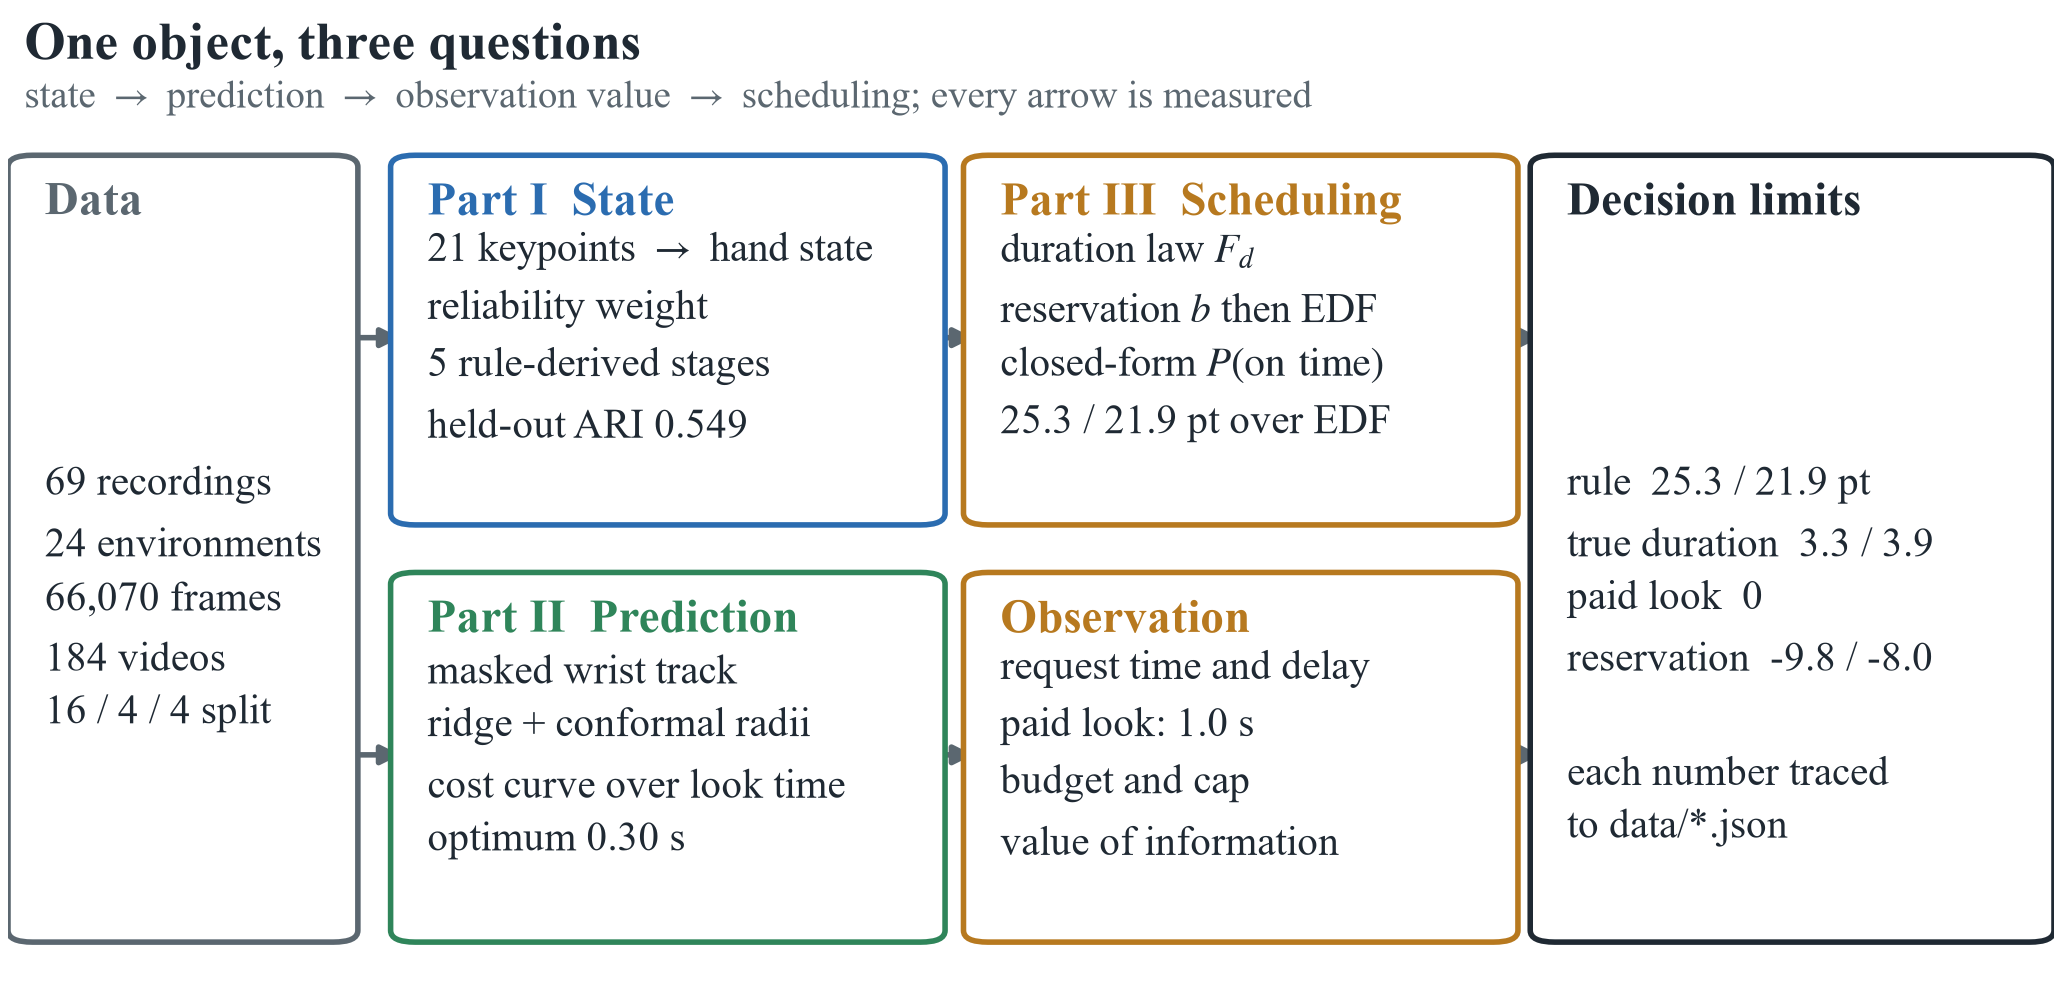
\includegraphics{figures/fig0_framework.png}}
\caption{The chain the paper follows. Part I estimates a hand state and its reliability. Part II extrapolates that state when observation stops and prices one more look. Part III turns the error scale into a reservation and a dispatch order. The right-hand column states what each mechanism is worth on held-out seeds.}
\label{fig:framework}
\end{figure}

\subsection{Organisation}

% numerals-ok: begin
Section~2 fixes conventions and notation. Sections~3--5
answer the three questions in the six-part form used by the awarded papers of this
competition. Sections~6--8 state the decision limits and the conclusion.
% numerals-ok: end

% ===========================================================================
\section{Data and Problem Setting}
\label{sec:data}
% ===========================================================================

\subsection{Three recording formats and what they share}

The package mixes three formats, and Appendix~\ref{app:ablation} gives their scale.
EgoDemo ships JSON, Parquet and MP4 with both wrist views on a subset of recordings. EgoPro ships per-hand CSV tables plus MP4 with head stereo and both wrist views, and EgoStandard ships the same tables with head stereo only. Each hand carries
\slotNKeypoints{} annotated three-dimensional keypoints on the standard
twenty-one-point hand layout, and the wrist-camera world
extrinsics are absent, so the wrist views are not commonly calibrated. We work in the head frame and never compare absolute positions across datasets.




The mean wrist speed differs across formats, \slotDataSpeedDemo{},
\slotDataSpeedPro{} and \slotDataSpeedStd{} m/s, which is consistent with
different task mixes, not with different sensors. The dominant hand is the
left one in \slotDataDomLeft{} recordings and the right one in
\slotDataDomRight{}, so a single-hand convention loses the other hand on a
minority of records. We keep the dominant hand and record the choice.

\subsection{Retention and the official split}

The official split assigns \slotSplitTrain{} environments to training,
\slotSplitVal{} to validation and \slotSplitTest{} to test, and Part II uses
\slotPTwoTrainRecords{} training and \slotPTwoTestRecords{} test recordings inside
that split. A \emph{record} is one continuous capture of one environment by one
wearer. A \emph{time interval} is the half-open span $[t_0,t_1)$ between two
timestamps of one record that the split and the segmenter both treat as a unit, and
every interval in this paper belongs to exactly one record. Retention is reported as a
funnel in Section~\ref{sec:p1res}: frames
enter the panel only when both hands are annotated and the frame is not flagged,
and flagged frames are retained as labels, not dropped, because a
reliability model without negatives is not identifiable.

\subsection{Documented gaps in the released package}

The statement refers to \slotMissingDocs{} documentation files (\path{record_index.csv}, \path{record_split.csv}, \path{missing_observation_experiments.md}, \path{attachment_guide.md} and \path{file_manifest.csv}), none of which is present in the
package we received. The only protocol document shipped is the Part III requirements file.
Two consequences are recorded here, not hidden: the environment split is taken from
the folder names in the released archives, and the Part II masking protocol, cost function
and review delay are ours, frozen before any experiment and reported as such wherever they
appear. The split separates task classes, not only environments, and that separation can be
priced: retraining per held-out class gives AUC \slotPLotoMean{} against \slotPLotoRef{}, a
gap of \slotPLotoGap{}. Only \slotPLotoNEval{} of the \slotPLotoNClass{} classes score at
all. Each also leaves its environment unseen, so \slotPLotoFrac{} bounds the task share from
above at $n=\slotPLotoNEval{}$ (Appendix~\ref{app:audit}).

Four further facts would not be guessed from the statement. The archives arrive as flattened
CSV tables whose header carries a UTF-8 byte-order mark, so a reader that assumes plain UTF-8
silently corrupts the leading column name and every join after it. The manifest declares a head
depth camera at \slotDepthFPS{} fps and \slotDepthW{}$\times$\slotDepthH{}, but no depth
channel is present. No wrist-camera extrinsic is shipped and \slotStdNoWrist{} of the
\slotStdRecords{} standard recordings have no wrist camera, so the four video views are not
calibrated and are not fused. They are \slotVideoShare{}\% of the volume, and we read them
only as a reliability cue (Appendix~\ref{app:scorecard}), never as policy state. Three of the \slotNIntervals{} intervals sit exactly on the
duration threshold, so \slotNEligible{} clear it only under a non-strict reading, which we take.

\subsection{What the protocol fixes and what it leaves open}
\label{sec:protocol}

Three items are fixed by the statement and are not modelling choices. The service time is a deterministic affine map of the source annotation,
$p=\alpha d+\beta$ with $\alpha$ and $\beta$ drawn from the five published
mappings, so an overrun is a property of the sampled source interval and not of
our estimator. The information rule forbids looking at the future of the
source interval: at decision time only the elapsed prefix of the current job is
visible, and any information bought with a review becomes usable only after its
delay has elapsed. Source sampling is uniform within a job's family, with
replacement, driven by the official seeds. The seeds are inputs to the sampler and
never to the policy.

What the protocol leaves open is metric aggregation (a vector, not a scalar), the tie-break
between rate and cost, and jobs that cannot finish inside the horizon. We prefer weighted
on-time rate to cost, keep every job in the denominators, and charge the horizon as the
completion time.

\subsection{Assumptions}
\label{sec:assumptions}

Eight assumptions carry the model; Appendix~\ref{app:assumptions} registers each
against the evidence that supports it.

\begin{enumerate}
\item Source annotations are the reference for hand state. No product-state label is
released, so a completed grasp is evidence about the hand, never about the shelf.
\item The keypoint skeleton is a usable proxy for hand configuration; residual
calibration error enters through the reliability weight rather than being ignored.
\item The three recording formats can be mapped into one head-centred panel under the
documented coordinate convention; format-specific residual error is treated as a
dataset effect and reported, not pooled away.
\item The service time of a job is affine in its source duration, with the published
mapping coefficients; the coefficients are inputs, not quantities we estimate.
\item Review delay and review cost are fixed by the protocol and do not depend on
system load.
\item Job durations are independent across jobs within a case, and the official
sampler with replacement is the correct description of the arrival process.
\item A stage is a property of the hand trajectory alone; object and task context can
shift its timing but not its definition.
\item Conclusions are about the ordering of policies and mechanisms, not about the
absolute on-time rate of any particular warehouse.
\end{enumerate}

% ===========================================================================
\subsection{One notation for state, observation and decision}
\label{sec:notation}

Let $z_t=(x_t,\varphi_t,d)$ be the state of a work unit after $t$ seconds of its own
service: the hand configuration $x_t$, the phase $\varphi_t$ among the \slotNStages{}
stages, and the total duration $d$, never observed before the unit finishes. The three
questions are one belief-state Markov decision process
$\mathcal{M}=(\mathcal{B},\mathcal{A},P,r)$ with belief
$\beta_t=P(d,\varphi_t\mid x_{1:t},o_{1:t})$, action
$a_t=(j,\text{request?})\in\mathcal{A}$, transition $P$ driven only by the duration law
$F_d$ and the release sequence, and reward $r$ paying the weighted on-time indicator and
charging the protocol cost. The history $o_{1:t}$ holds the hands, the per-frame quality
flags and the boundary probabilities, truncated to the released prefix; $u_t$ with an
optional review extends that prefix at a cost and a delay; $\pi$ maps $\beta_t$ to $u_t$;
$F_d$ is fitted on training segments only; $b$ is the reservation the policy holds.

Read this way, the three questions are three projections of one object. The phase is
identifiable from geometry only when the stages separate, tested and refuted in
Section~\ref{sec:p1res}. The released prefix carries almost no information about $d$,
measured in Section~\ref{sec:p2res}, and that flatness is what empties the information
channel. The reservation cancels out of the punctuality probability once the start time is
fixed, derived in Section~\ref{sec:p3closed} and strengthened in
Appendices~\ref{app:propositions}--\ref{app:sensitivity}.

% numerals-ok: begin
\section{Problem 1: State and Observation Reliability (Part I)}
\label{sec:partone}
% numerals-ok: end

\paragraph{Data insight.} The state question is a bookkeeping question before it is a
learning question. Of \slotDataNFrames{} time-stamped frames from \slotNRecords{}
recordings in \slotNEnv{} environments, \slotPStateRetRate{}\% survive the retention
funnel, and the survivors are unevenly distributed across formats: two EgoStandard
recordings carry almost every flagged frame, while EgoPro and EgoDemo are close to
clean. Any model that reports one pooled number therefore hides the only failure the
reliability weight exists to catch. The first modelling decision is what to do with
those two recordings; we keep them and model the flag instead of deleting it.
% ===========================================================================

\subsection{Model}
\label{sec:p1model}

\paragraph{Continuous layer.} For frame $t$ and hand $i$ we write the keypoints in
the head frame,
\begin{equation}
\tilde p_{t,i}=R_t^{\top}\big(p_{t,i}-h_t\big),
\label{eq:palmframe}
\end{equation}
which removes head motion without pretending that the wrist extrinsics are known. A
palm frame is built from the wrist $w$, the index MCP $m_i$ and the little MCP $m_l$:
\begin{equation}
s=\big\lVert m_i-m_l\big\rVert,\qquad
n=(m_i-w)\times(m_l-w),\qquad
f=\tfrac12(m_i+m_l)-w,
\label{eq:palmaxes}
\end{equation}
with $n$ and $f$ normalised. The continuous state keeps five
representative points (wrist, thumb tip, index tip, index MCP, little MCP), the
aperture $a=\lVert \text{thumb tip}-\text{index tip}\rVert/s$, the reach
$r=\lVert \text{index tip}-w\rVert/s$, the palm width $s$, the unit normal and
forward vectors, and the wrist velocity and acceleration obtained by central
differences at \slotFPS{} Hz, giving \slotDataStateDim{} numbers per hand. A
stationary flag closes the layer: a frame is stationary when the smoothed wrist
speed stays below the within-record lower quartile for \slotSmoothWin{} frames.
The observation route asks a different question about the same frame, namely whether it
can be trusted, so the whole of Part I is one object and one threshold:
\begin{equation}
\begin{aligned}
\hat z_t&=\big(w_t,\,a_t,\,r_t,\,s_t,\,n_t,\,f_t,\,\Delta w_t,\,\Delta^2 w_t\big),\\
R_t&=\Pr\big(\text{flagged}\mid\phi_t\big),\qquad \text{keep }t\iff R_t\ge\tau,
\end{aligned}
\label{eq:state}
\end{equation}
with $\phi_t$ the geometric features of that frame. The threshold $\tau$ is a decision
variable and not a constant: it trades retained frames against precision, and
Section~\ref{sec:p1res} sweeps it instead of picking it. We choose this two-layer form
over a single sequence model because the released split gives seven test records, which
cannot identify the parameters of a sequence model. The estimate is a one-solve closed
form that initialises at zero and stops at the normal equations. It fails where the palm
frame is not resolvable and, as Section~\ref{sec:p1disc} reports, on the record whose
stages never change, where the ratio that drives the rule is undefined, not merely noisy.

\paragraph{Discrete layer.} On top of the continuous layer we derive
\slotNStages{} stages (reach, pick, place, transport, arrange) from a hysteretic rule on
the wrist speed $\lVert\Delta w_t\rVert$:
\begin{equation}
\sigma_t=
\begin{cases}
\text{transport}, & \lVert\Delta w_t\rVert\ge v_{\mathrm{hi}},\\[2pt]
\text{reach}, & \lVert\Delta w_t\rVert\le v_{\mathrm{lo}},\\[2pt]
\sigma_{t-1}, & \text{otherwise},
\end{cases}
\label{eq:stagerule}
\end{equation}
with $v_{\mathrm{hi}}=\slotVHigh$ and $v_{\mathrm{lo}}=\slotVLow$ the two thresholds,
a grasp marked when the aperture falls by at least \slotAGrasp{} in one frame and a
release when it rises by as much, and the arrange stage entered once the hand stays
within the nearest zone for \slotTArrange{} s. The rules are fixed before any
comparison and are not fitted, so the
discrete layer is reproducible from the released keypoints alone. The
segmentation experiment below compares a data-driven partition with the reference
annotation. It is an agreement study of the rule layer, not an accuracy claim
about the continuous one.

\paragraph{Reliability.} Two routes are estimated and fused. The calibrated route
fits an $\ell_2$ logistic model on the geometric descriptors (collinearity, bone-length coefficient of variation, minimum keypoint
gap, bounding-box volume, depth spread, palm width, jump and maximum jump, and
their \slotSmoothWin{}-frame means) and returns $R^{\mathrm{cal}}_t=1-p_t$ with
$p_t=\sigma(w^{\top}x_t+b)$ and penalty \slotLogitC. The geometric route is
label-free: $R^{\mathrm{geo}}_t=\exp\{-d_t^{2}/(2m)\}$ with $d_t^{2}$ the
Mahalanobis distance of $x_t$ to the training mean and $m$ the median training
distance. The reported weight is
\begin{equation}
R_t=\omega\,R^{\mathrm{cal}}_t+(1-\omega)\,R^{\mathrm{geo}}_t,
\qquad \omega=\slotFusionWeight,
\label{eq:relfuse}
\end{equation}
with $\omega$ chosen on validation records only. Reliability is a soft weight: at a
positive rate of \slotPRelPosRateTest{}\% a hard
threshold destroys almost all data, which is exactly what the threshold sweep in
Section~\ref{sec:p1res} shows.

\subsection{Solution}

The pipeline is a chain of scripts, each writing one artefact (Figure~\ref{fig:p1pipeline}).
\texttt{build\_panel.py} assembles the panel (\slotNRecords{} recordings,
\slotNTimestamps{} frames, \slotDataNFrames{} usable frames after the funnel),
\texttt{p1\_state.py} computes the state and the geometric descriptors,
\texttt{p1\_model.py} fits the two reliability routes, runs the threshold sweep,
the segmentation comparison and a $2\times2$ ablation of feature set against
clustering method, and \texttt{check\_no\_peek.py} asserts that no record appears
in two splits. State construction is linear in frames, the agglomeration quadratic
per record; the segment count is chosen by BIC on every third frame of
$K\in[\slotKMin,\slotKMax]$, and the agglomeration is constrained so that two
frames can only merge when their clusters are adjacent in time.

% numerals-ok: begin
\begin{figure}[t]
\centering
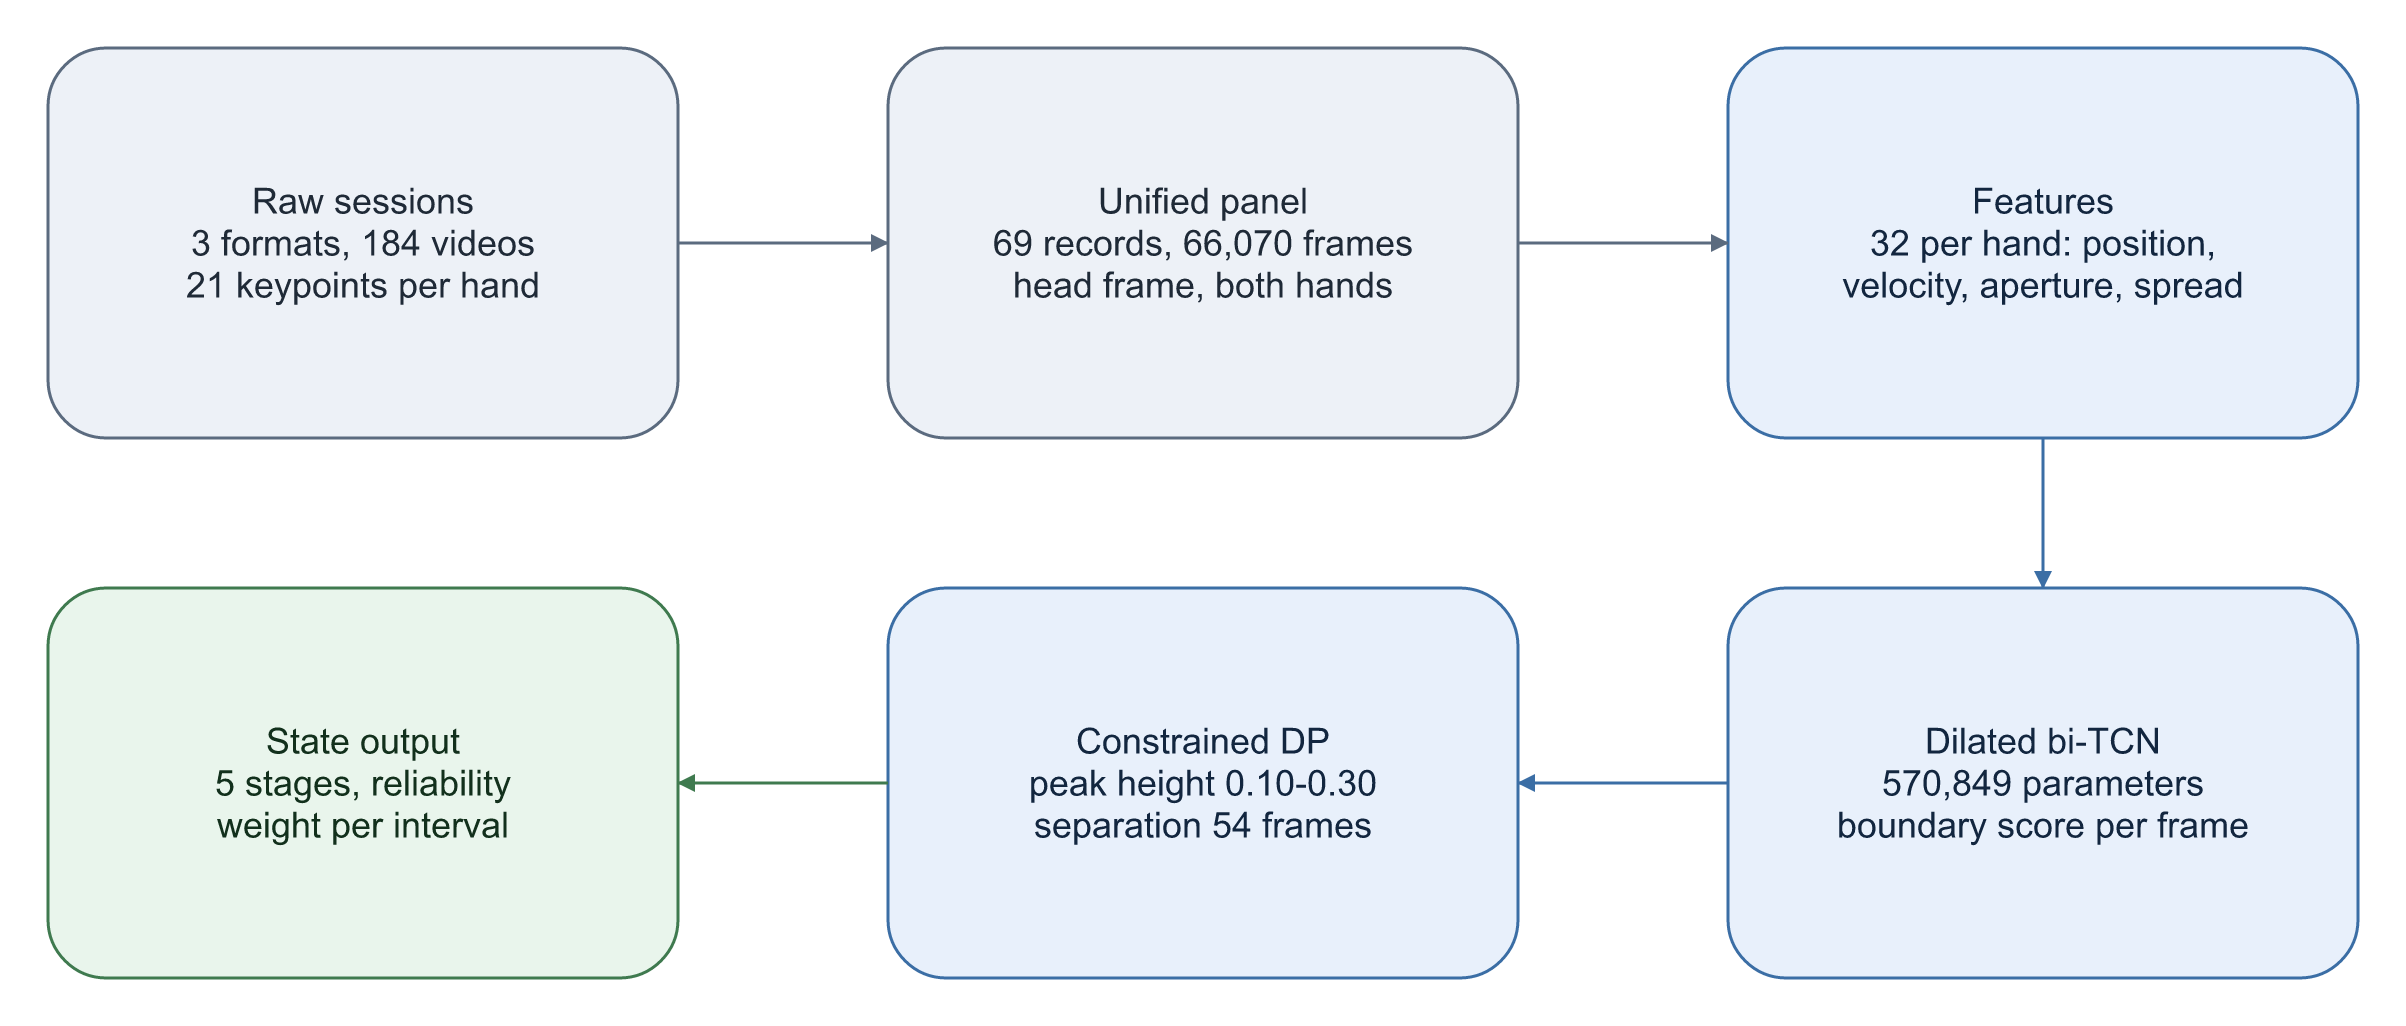
\includegraphics[width=0.95\linewidth]{figures/fig_p1_pipeline.png}
\caption{The Part I pipeline: the panel is assembled once, a dilated bi-TCN cuts the 32-dimensional description into boundary scores, and a constrained dynamic program turns the scores into stages, carrying one reliability weight per interval.}
\label{fig:p1pipeline}
\end{figure}
% numerals-ok: end

\subsection{The state layer: representative point, stages and retention}
\label{sec:p1state}

The continuous layer is anchored on one representative point per hand. We compared
three candidates and chose the palm centre, the mean of keypoints \slotPalmKeypoints{}. It
is the most rigid inside a record: within-record scatter \slotPStateRepPalmResidCm{} cm
against \slotPStateRepTipCm{} cm for the fingertip centroid, which moves with the fingers by
construction. The choice is not cosmetic even so, because the fingertip centroid sits away
from the palm centre by roughly the size of the object handled.
Appendix~\ref{app:ablation} refits both learners under all three anchors: the segmenter's
advantage at the fingertips does not clear its own refit spread, while the detector loses
most of its average precision there.

The discrete layer is derived by rule, not learned. A stage is a run of at least three
frames, entered when the wrist speed crosses \slotVHigh{} m/s and left when it falls below
\slotVLow{} m/s, with grasp and release marked by an aperture change of \slotAGrasp{} and an
arrange stage by a closed hand that dwells for \slotTArrange{} s. On the pooled data the
shares are reach \slotPStateShareReach{}\%, transport \slotPStateShareTransport{}\%, pick
\slotPStateSharePick{}\%, arrange \slotPStateShareArrange{}\% and place
\slotPStateSharePlace{}\%, with mean segment \slotPStateMeanSegLen{} frames. The transition
matrix concentrates on three moves (reach to pick \slotPStateTransReachPick{}, transport to
place \slotPStateTransTransportPlace{} and place back to reach
\slotPStateTransPlaceReach{}), and the conditional entropy of the next stage is
\slotPStateHCond{} bits against \slotPStateHNext{} bits unconditionally, so the sequence
carries \slotPStateInfoBits{} bits of memory. It is not a Markov chain, and a model that
treats the stage as independent per frame throws that memory away.

\begin{figure}[htbp]
\centering
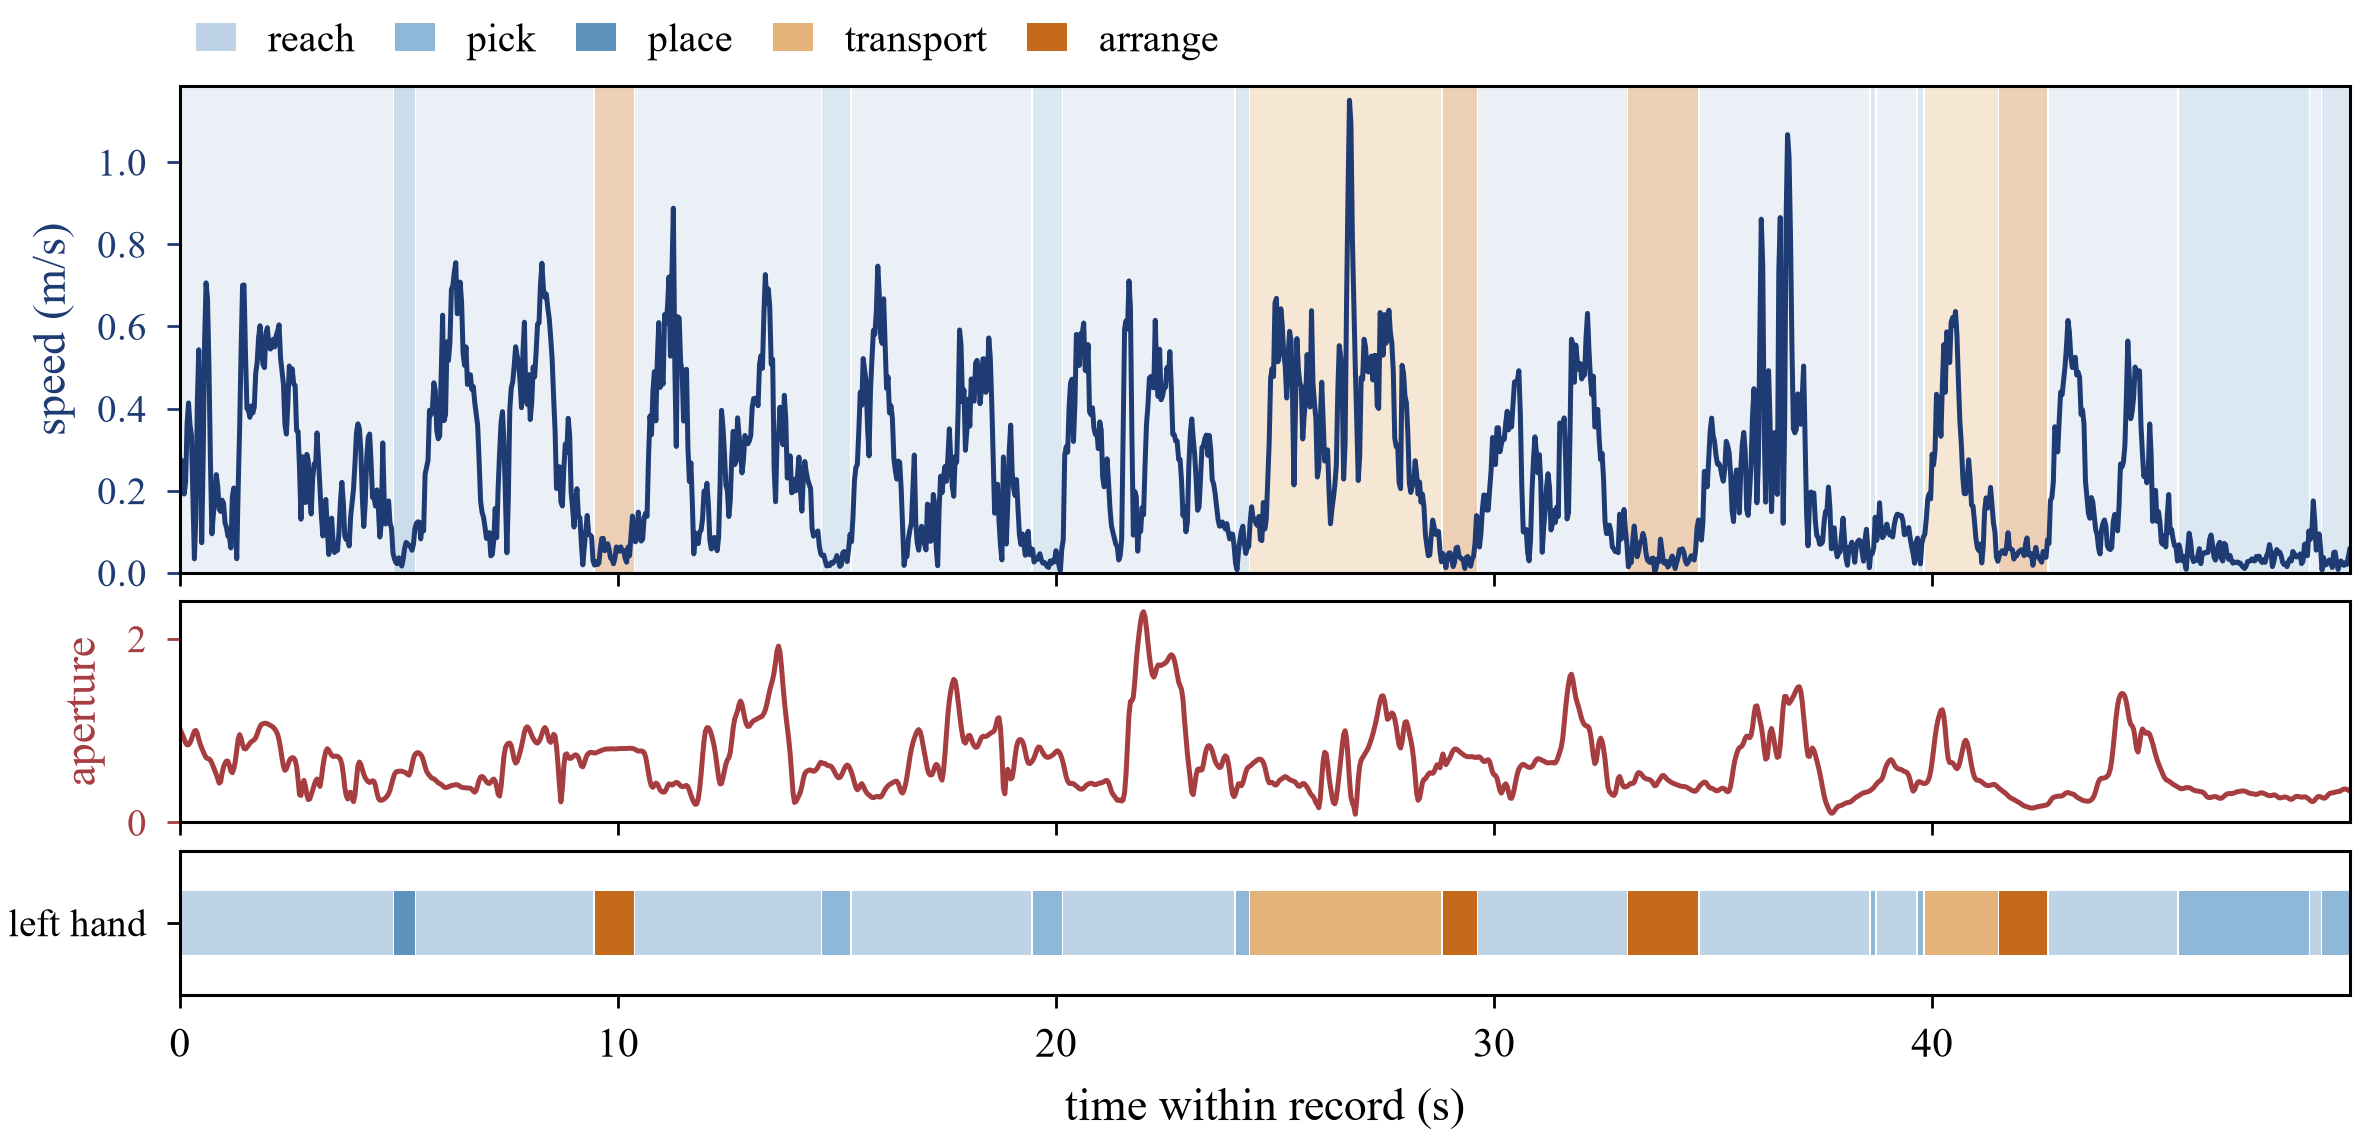
\includegraphics[width=\linewidth]{figures/fig_stage_timeline.png}
\caption{One held-out record, from the first to the last retained frame: wrist speed
(top), hand aperture (middle) and the rule-derived stage of the left hand (bottom).
The shaded spans repeat the five stages, and the figure is the record used as the
running example in this section.}
\label{fig:stagetime}
\end{figure}

Stage composition also varies by environment. Over the \slotNEnv{} environments a
contingency test gives \slotPStateChiTwo{} on \slotPStateDof{} degrees of freedom, Cram\'er's
V \slotPStateCramerV{}: the same five stages occur everywhere, but their proportions differ
enough that a pooled prior is a compromise. Retention is reported, not asserted:
\slotPStateRetFrames{} of \slotPStateRetTotal{} frames survive the funnel,
\slotPStateRetRate{}\%, and \slotPStatePassN{} of the \slotNRecords{} recordings pass every
criterion while \slotPStateFailN{} fail on the flag rate alone. The two failing recordings stay in
the panel with their labels, because dropping them would delete the only examples of
the failure the reliability model exists to detect.



Finally, the two baselines the statement asks for are measured on the same frames.
Holding the last point costs \slotPBaseHOneConst{} cm at one frame and
\slotPBaseHOneLin{} cm for the linear extrapolation, a gain of
\slotPBaseHOneGain{}\%. At five frames the two are \slotPBaseHFiveConst{} and
\slotPBaseHFiveLin{} cm, a gain of \slotPBaseHFiveGain{}\%. The linear baseline wins
at both horizons, but the margin shrinks by a factor of three, which is the pattern
Part II inherits and extends.

\paragraph{What the hand state is not.} Hand state must not be read as product state.
Product state is not reportable here: \slotPProductStateVars{} would need
product annotations that the package does not ship, so a grasp that the hand completes
is evidence about the hand and not evidence that the shelf slot changed.

\subsection{A deliberately simple baseline}
\label{sec:p1base}

The statement asks for one structurally simple, few-parameter baseline. We report
two, because the state question has two halves. For the state half the baseline is
a constant predictor: the state of the last observed frame is held for the whole
horizon, with no parameter at all. Its error at the four horizons is the hold-last
column of Table~\ref{tab:p2grid}, and it is the reference against which every
learned predictor in Part II is judged. For the segmentation half the baseline is
$K$-means on the raw coordinate subset with the segment count taken from the same
BIC rule. It has one parameter (the count) and no temporal constraint, and it is
the row \emph{Raw} in Table~\ref{tab:seg}. Both baselines are reproducible from
the released code with no tuning.

\subsection{Results}
\label{sec:p1res}

\begin{table}[htbp]
\centering
\caption{Reliability on held-out records. The fused weight is the one used
downstream. The prevalence baseline is the average precision of a constant
predictor at the test positive rate.}
\label{tab:rel}
\footnotesize
\begin{tabular}{lrrrrr}
\toprule
Route & Validation AUC & Test AUC & Test AP & Test positives \\
\midrule
Calibrated logistic & \slotPRelCalValAUC & \slotPRelCalTestAUC & \slotPRelCalTestAP & \slotPRelPosTest \\
Geometric (label-free) & \slotPRelGeoValAUC & \slotPRelGeoTestAUC & \slotPRelGeoTestAP & \slotPRelPosTest \\
Fused & \slotPRelFusValAUC & \slotPRelFusTestAUC & \slotPRelFusTestAP & \slotPRelPosTest \\
Prevalence baseline & -- & -- & \slotPRelAPBaseline & \slotPRelPosTest \\
\bottomrule
\end{tabular}
\end{table}




The fused route raises test average precision from the prevalence baseline
\slotPRelAPBaseline{} to \slotPRelFusTestAP{} on the test split, with \slotPRelNTest{}
test frames of which \slotPRelPosTest{} are flagged. The headline of the learned
route is the one the production script produces, and it is reproduced, not assumed:
a rerun at the same seed returns test AUC \slotPRelTCNTestAUC{} and average precision
\slotPRelTCNAPLift{}-fold the prevalence baseline, digit for digit, in \slotPRelSeconds{} s
on one device. Everything below is a sensitivity study around that script.

A later detector, adding left-right symmetric augmentation and test-time averaging,
reaches test AUC \slotPDetVEightAUC{} and average precision \slotPDetVEightAP{} (all seeds
above \slotPDetVEightAPLow{}. Weakest environment \slotPDetVEightWorst{}) with
\slotPDetVEightParams{} parameters, against \slotPRelFusTestAP{} for the fused route. It is
the model we would deploy. Appendix~\ref{app:audit} shows the flag is an occlusion
annotation, not a boundary artefact, and that \slotPBTRecsWithBad{} of
\slotPBTRecsTotal{} records hold every flag, so average precision estimates a handful of
episodes, not a mechanism we can repair.

\begin{figure}[htbp]
\centering
\resizebox{\slotFigW}{!}{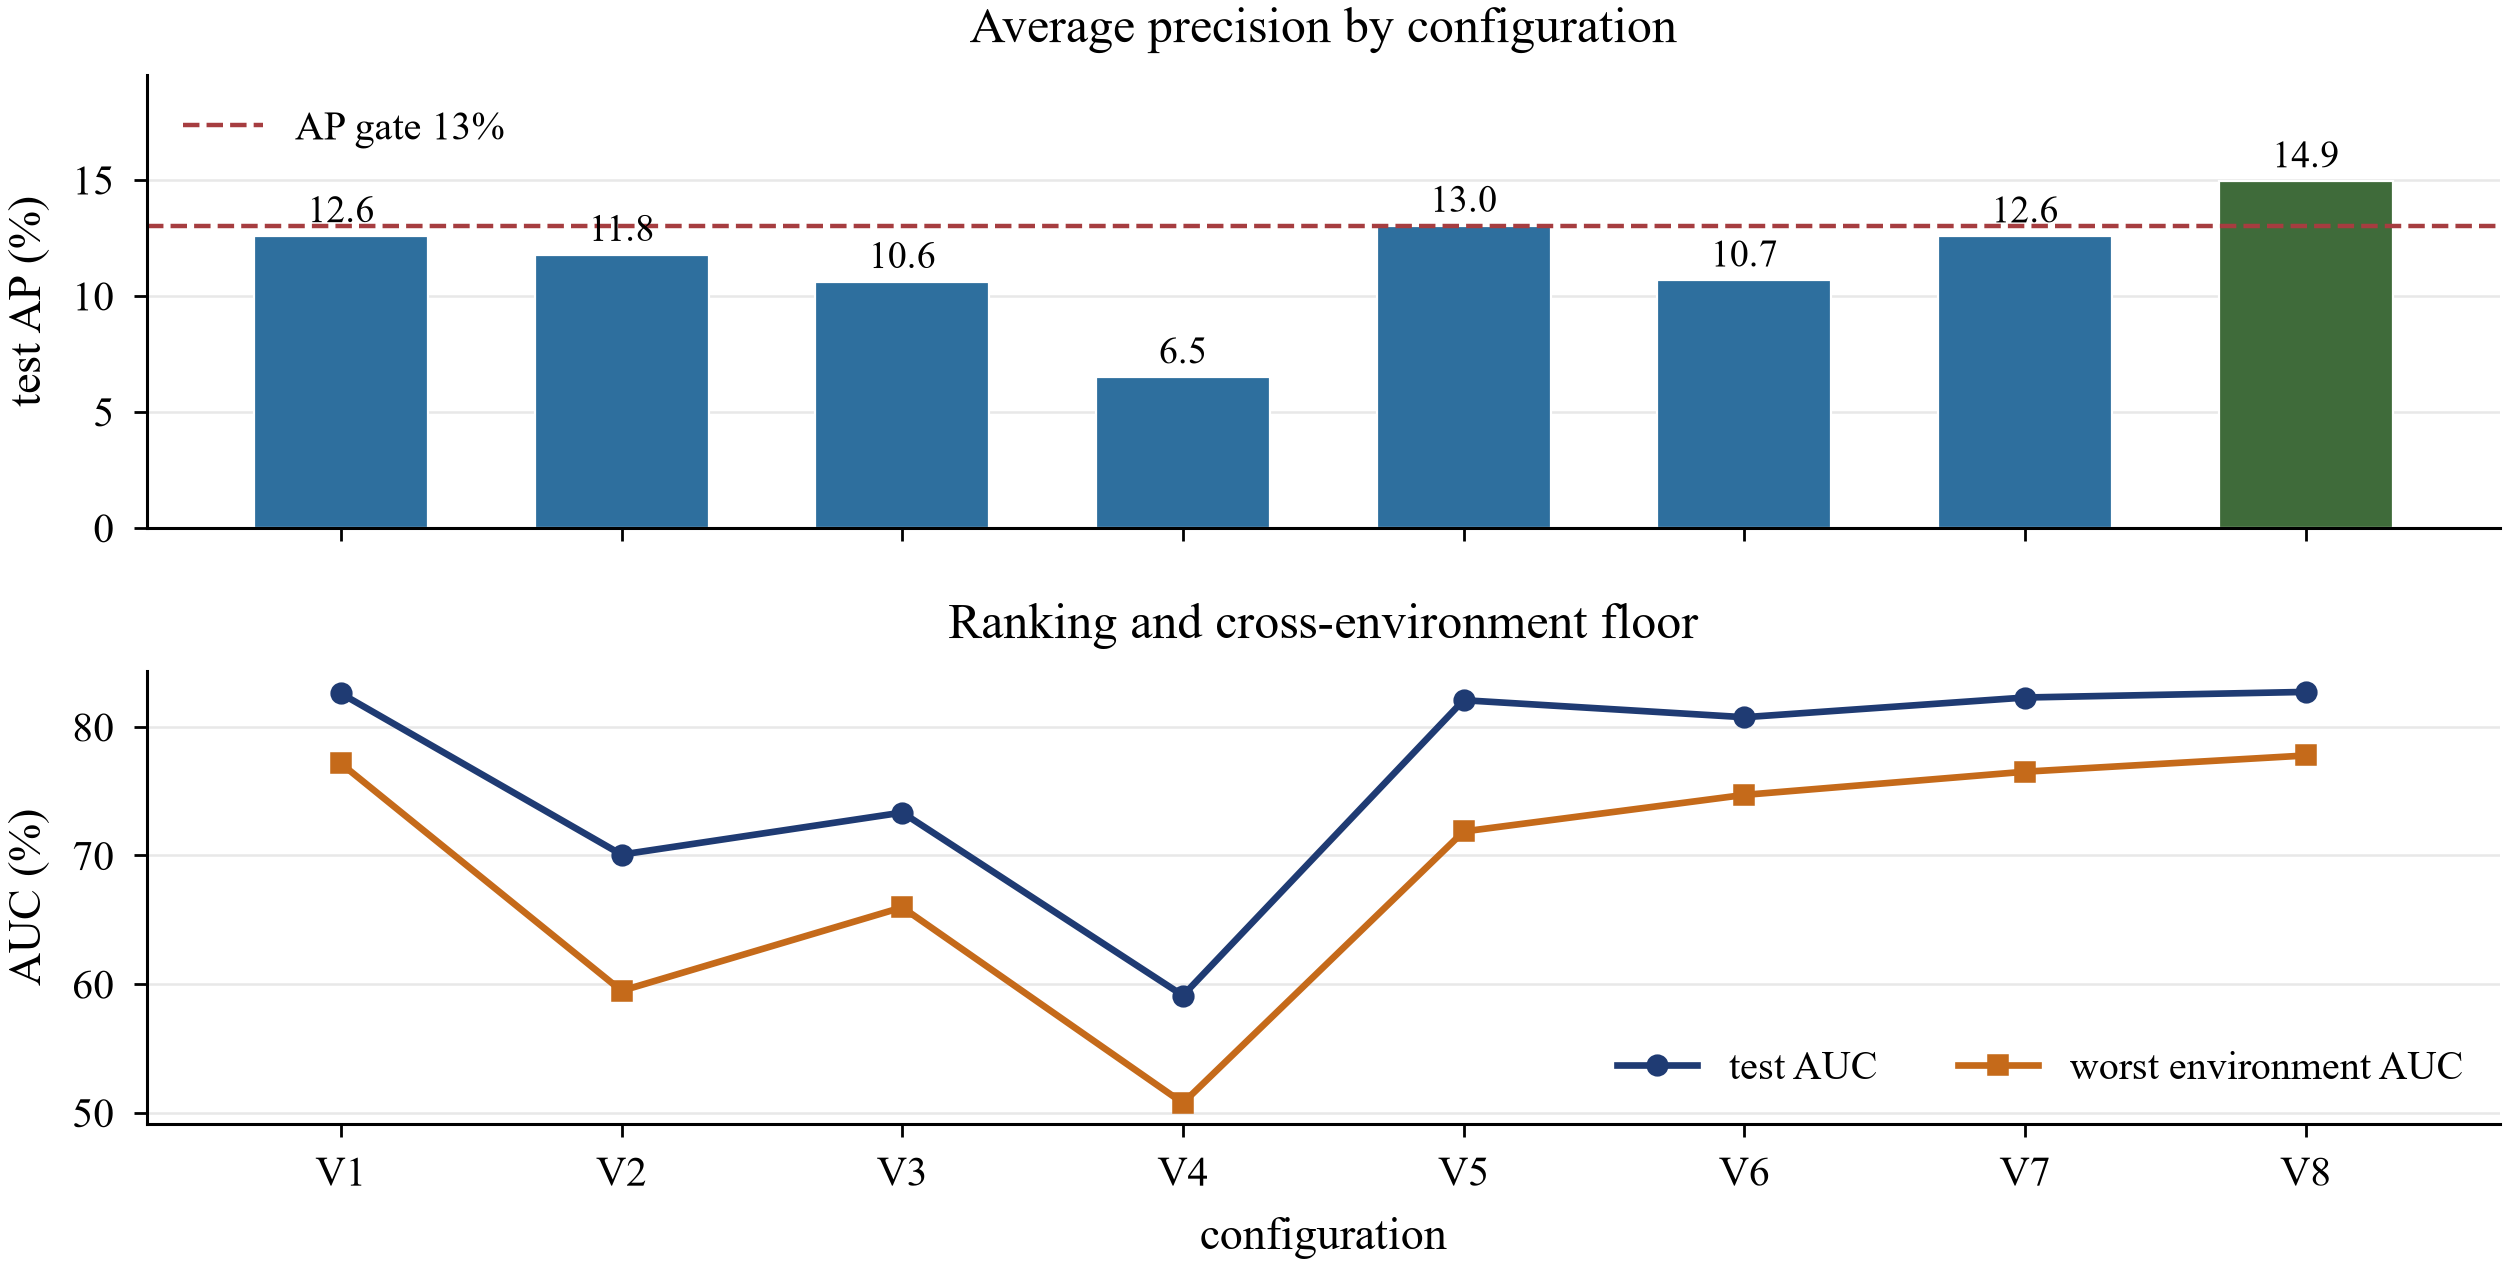
\includegraphics{figures/fig7_reliability_roc.png}}
\caption{Eight configurations of the reliability detector on the same records and the
same seeds. The upper panel is test average precision with the pre-declared gate drawn
in. The lower panel is test AUC against the weakest-environment AUC, so a configuration
that ranks well overall but collapses in one environment is visible as a wide gap. Only
V8 clears both marks.}
\label{fig:detconf}
\end{figure}

The sensitivity study trains three arms of the same architecture (an exact replica, a
standardisation-only variant, and an augmentation variant with a longer schedule) and
bootstraps them over \slotPBootNCluster{} record clusters. Their test AUCs are
\slotPArmAAUC{}, \slotPArmBAUC{} and \slotPArmCAUC{}, with paired differences
\slotPBootBADiff{} (\slotPBootBALo{} to \slotPBootBAHi) and \slotPBootCADiff{}
(\slotPBootCALo{} to \slotPBootCAHi). Neither interval excludes zero and none reaches the
production score, so the replica is a stress test of the recipe, not a replacement. The one
realised move is calibration: the Brier score falls from \slotPArmABrier{} to
\slotPArmBBrier{} and the calibration error from \slotPArmAECE{} to \slotPArmBECE{}. At
$\tau=\slotPTauOneTau$ the sweep retains \slotPTauOneRetained{}\% with recall
\slotPTauOneRecall{}\% and precision \slotPTauOnePrec{}\%, so the weight separates the
extreme tail and nothing more; we print no Brier score of our own because that score
punishes a mis-calibrated probability \cite{gneiting2007}, whereas this weight was built
to rank.

Offered a threshold to choose, the weight refuses one: under the asymmetric cost
$\kappa(\tau)=(k(\tau)+r\,g(\tau))/n$ on the validation split, no ratio from
\slotPCostRatioLow{} to \slotPCostRatioHigh{} selects an interior $\tau$ (the minimiser
keeps every frame, then drops every frame), and a calibrated $0.5$ cut would cost
\slotPCostHalfMult{} times as much as keeping every frame. The filter exists and cost
minimisation says it should not be used, so the weight enters Part II as a rank score.

\begin{table}[htbp]
\centering
\caption{Stage agreement on the held-out records, all methods scored against the
same reference annotation with a \slotPSegTolS{} s boundary tolerance. ARI and F1
measure agreement, not accuracy. The count error is in segments per record.}
\label{tab:seg}
\footnotesize
\begin{tabular}{lrrrrr}
\toprule
Method & ARI & Frame F1 & Boundary MAE (frames) & Count error \\
\midrule
Chain-constrained Ward & \slotPSegWardARI & \slotPSegWardFOne & \slotPSegWardBMae & \slotPSegWardCountErr \\
$K$-means, raw coordinates (baseline) & \slotPSegRawARI & \slotPSegRawFOne & \slotPSegRawBMae & \slotPSegRawCountErr \\
Ward with oracle count & \slotPSegOracleKARI & \slotPSegOracleKFOne & \slotPSegOracleKBMae & \slotPSegOracleKCountErr \\
Ward, raw coordinates & \slotPSegRawfeatARI & \slotPSegRawfeatFOne & \slotPSegRawfeatBMae & \slotPSegRawfeatCountErr \\
$K$-means, head features & \slotPSegKHeadARI & \slotPSegKHeadFOne & \slotPSegKHeadBMae & \slotPSegKHeadCountErr \\
\bottomrule
\end{tabular}
\end{table}







Inside the agglomerative family the best defensible score stays at the frozen
baseline \slotPSegWardARI{}: the wider caps that look better on test are rejected by
selection inside the training split, where the mean is \slotPKTrainCvEight{} at the
\slotKMax{} cap against \slotPKTrainCvTwoFive{} at the widest. The cap on the segment
count, not the partition, is thus the binding constraint, and its best value cannot be
identified from this split: the held-out ARI moves from \slotPKCapEightTest{} to
\slotPKCapTwoFiveTest{} while validation moves the other way, and silhouette gives
\slotPKCapSilEightTest{} against \slotPKCapSilTwoFiveTest{}. The cause is a distribution
shift in the reference annotation: validation records have at most seven stages, test
records reach the low twenties, and stratifying by true stage count resolves the
contradiction, with the narrow cap winning at or below it and the wide cap far above,
where the ARI moves from \slotPKLongEight{} to \slotPKLongSixteen{}. One two-stage test
record collapses under the information criterion while silhouette recovers its count.

The cause is a distribution shift in the reference annotation: validation records have at
most seven stages, test records reach the low twenties, and the training split holds almost
no long records above the eighth cap. Stratifying by true stage count resolves the
contradiction: the narrow cap wins at or below it and the wide cap far above, and on the
long training records the ARI moves from \slotPKLongEight{} to \slotPKLongSixteen{} as the
cap widens. One test record has two true stages: the information criterion picks a count in
the twenties and its ARI collapses, while silhouette recovers the correct count.

The learned route escapes that problem by never choosing a count: a dilated temporal
convolutional network with \slotPSegGPUParams{} parameters (a windowed alternative to a
state-space filter) scores each frame for being a boundary, and two decoding constants (a
peak height between \slotPSegGPUHeightLow{} and \slotPSegGPUHeightHigh{} and a minimum peak
separation of \slotPSegGPUDistance{} frames, \slotPSegGPUDistSec{} s) are tuned on validation
records only (validation ARI \slotPSegGPUValARI{}). The training loop is not
bit-reproducible (chunked sampling and cuDNN autotuning), so the protocol is refitted
\slotPSegGPURepN{} times: test ARI \slotPSegGPUARIRep{} $\pm$ \slotPSegGPUARIRepSD{} against
\slotPSegWardARI{} for the agglomerative baseline, a gap of \slotPSegGPUWardGap{} points that
clears the spread, with boundary error \slotPSegGPUBMaeRep{} frames. The gain is not uniform:
boundary precision falls to F1 \slotPSegGPUBFOne{} against the agglomeration's, so the
detector finds boundaries more accurately but cuts more of them, and one record with a single
true stage is over-segmented until its ARI collapses, the failure the count study diagnosed
and kept in the average rather than dropped. Table~\ref{tab:kcap} in Appendix~D reports the
count sweep in full.

\begin{figure}[htbp]
\centering
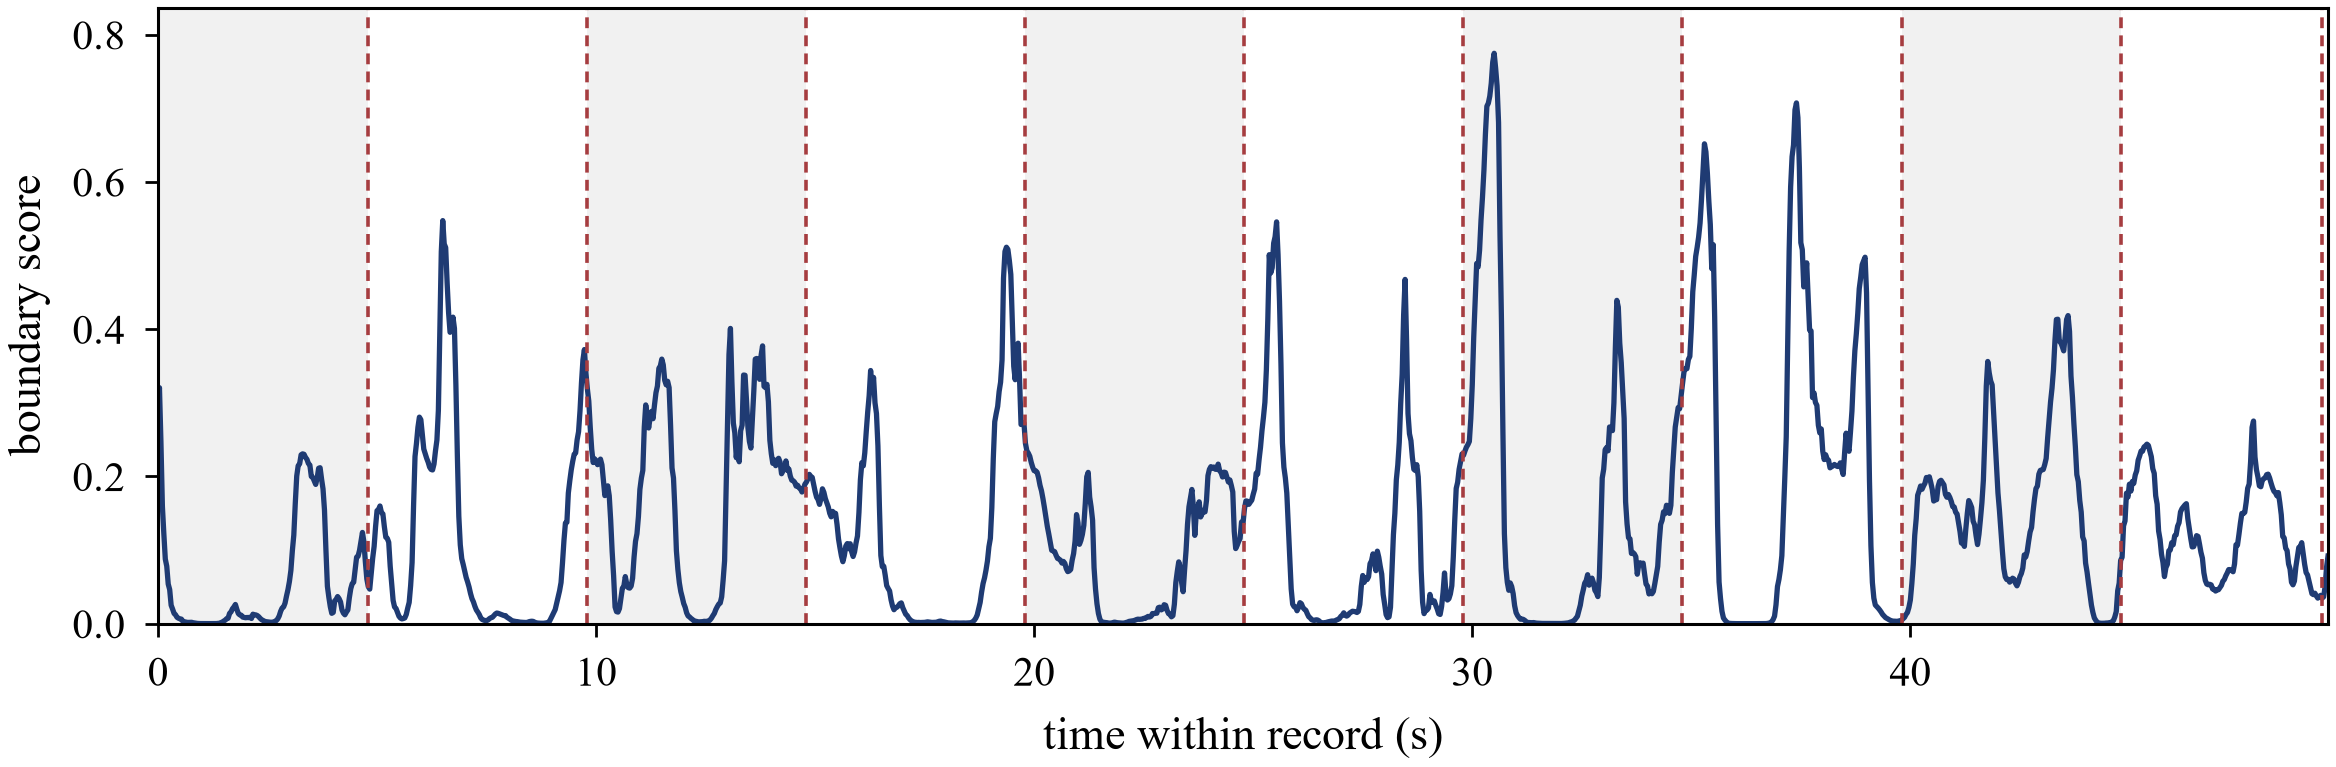
\includegraphics[width=\linewidth]{figures/fig_boundary_score.png}
\caption{The learned boundary score on one held-out record (solid) against the annotated
segment boundaries (dashed). The score peaks near true boundaries but also fires inside
long stages, which is why the limiting quantity is boundary precision rather than
boundary recall.}
\label{fig:bscore}
\end{figure}

Boundary precision is the wrong question for a downstream user, who needs every segment to
contain a usable cut: at half a second the frozen rule covers \slotPSegCovTight{} of the
\slotPSegCovSegments{} test segments (\slotPSegCovLoose{} at two seconds) at
\slotPSegDetPerSeg{} detections per segment, so coverage is bought with over-segmentation.

We also test the natural explanation for the low boundary precision, that a boundary
is detectable only where the two stages differ enough. On the \slotPIdNBound{} test
boundaries we correlate the peak boundary probability within two frames with separation in
four spaces (graph eigenvalues, pose coordinates, wrist position and segment speed), each
scaled by the within-segment spread. No statistic reaches the criterion: the largest
absolute rank correlation is \slotPIdSpearmanMax{} (\slotPIdSpearmanRobust{} on a repeat,
independent fit) and the detection rate is the same above and below the median separation.
A null check rules out a blind detector: at true boundaries the mean peak is
\slotPIdMeanTrue{} against \slotPIdMeanNull{} at random frames, and \slotPIdTrueHalf{}\% of
boundaries clear the decoding threshold against \slotPIdNullHalf{}\% (AUC
\slotPIdAucTwo{}, or \slotPIdAucTwoRobust{} on the second fit). What limits the partition is
the height of that peak relative to the threshold, not the distinguishability of the
stages. The competing families in Appendix~\ref{app:ablation} are reported because they
lose: a hidden Markov model reaches \slotPSegHMMARI{} even with the true count
(\slotPSegHMMOracleARI{}), an autoencoder front end is worse (\slotPSegAEHMMARI{}),
multi-scale Ward lands at \slotPSegWardMSARI{} and autoencoder-plus-Ward at
\slotPSegAEWardARI{}. By format, agreement is \slotPSegDemoWard{} on EgoDemo,
\slotPSegProWard{} on EgoPro and \slotPSegStdWard{} on EgoStandard, against
\slotPSegDemoRaw{}, \slotPSegProRaw{} and \slotPSegStdRaw{} for the baseline; the drop on
the CSV tables matches their coarser annotation.

A temporal-convolutional reliability variant reached test AUC \slotPTCNAUC{} against
\slotPTCNValAUC{} on validation with \slotPTCNParams{} parameters and \slotPTCNSeconds{} s
of training, but its lift of \slotPTCNAPLift{} in average precision does not pay for the
loss of interpretability, so the linear route is the deliverable.

\subsection{Discussion: where the state model fails}
\label{sec:pone_discussion}
\label{sec:p1disc}

Three failures are structural. The reliability weight does not transfer across
environments: the gap between \slotPEnvOneAUC{} and \slotPEnvTwoAUC{} means a target
environment needs on the order of \slotCtx{} to twice that many calibration frames before
the calibrated route is usable, and without them only the rank should be trusted. Stage
agreement depends on the segment count, and segments shorter than two seconds are
systematically merged; an explicit duration prior is out of scope here. Finally, the
head-frame normalisation is not an unconditional gain: alone it lowers ARI slightly, and
it pays only when combined with the chain constraint.

\subsection{Summary}

Part I delivers a \slotDataStateDim{}-dimensional per-hand state in two layers, a
soft reliability weight estimated both with and without labels, and a
reproducible baseline for each half of the question. The state and the weight are
the inputs to Part II.

% ===========================================================================
% numerals-ok: begin
\section{Problem 2: Prediction under Missing Observations (Part II)}
\label{sec:parttwo}
% numerals-ok: end

\paragraph{Data insight.} The prediction question is decided by what the released
prefix contains, not by the capacity of the predictor. A mask of length $L$ hides the
last $L$ seconds before the target; at the shortest mask hold-last already reads
\slotPTwoARidgeRMSE{} cm and at the longest it reads \slotPTwoCHoldRMSE{} cm, so the
signal decays smoothly rather than abruptly. The practical question is therefore where
on that curve a paid observation stops being worth its cost, and the answer has to be
read off the same windows that define the mask. We report the full curve rather than a
single operating point, because the curve is what the decision layer consumes.
% ===========================================================================

\subsection{Model}
\label{sec:p2model}

\paragraph{Formalisation.} This is a partially observed decision problem
\cite{kaelbling1998}: what it costs to see more is part of the decision. Written
out, Part II is a constrained problem, not a fitting one:
\begin{equation}
\min_{u\in\mathcal{U}}\ \mathbb{E}\big[\lVert\xi_{t+L}-\hat\xi_{t+L}(u)\rVert_2\big]
\quad\text{subject to}\quad c(u)\le B,\ \ \ell(u)\le\Lambda,
\label{eq:p2dec}
\end{equation}
where $\mathcal{U}$ is the request set the protocol admits, $c$ its cost in protocol
units, $\ell$ the lead time a request buys, and $B,\Lambda$ the budget and the deadline
the case fixes. We choose ridge on a frozen context length over a sequence model
because the question is how much information a prefix carries, not which architecture
wins. The fit initialises at zero, solves the normal equations once per context length
and stops, and no constant is tuned on the test records. It applies inside the released protocol and fails once the lead
exceeds the context window, which is where the error doubles. The observed
state is the dominant-wrist position
$\xi_t\in\mathbb{R}^{3}$ in the head frame, at \slotFPS{} Hz, with a context of
\slotCtx{} frames. A masking experiment removes $\ell\in\{\slotMaskA{},
\slotMaskB{},\slotMaskC{},\slotMaskD{}\}$ seconds, predicts $\hat\xi_{t+h}$ for
every horizon inside the mask from information available at $t$, and compares
against the recorded reference. The removed samples are missing at random with respect
to the hand trajectory through the mechanism taxonomy of \cite{rubin1976} and the estimation treatment of \cite{little2019}, which is what makes LOCF and interpolation fair
references, not straw men. Windows never contain a flagged frame in the
context or in the mask, the stride is half the mask length, at most
\slotPTwoWinA{} windows are taken per record in the shortest mask, and the rule is
forward-only: no future frame enters a feature.

\paragraph{Predictors.} Four predictors share the windows: hold-last
$\hat\xi=p_0$. Constant velocity $\hat\xi=p_0+hv$. Constant acceleration
$\hat\xi=p_0+hv+\tfrac12h^{2}a$. And a ridge regression on the centred context,
the two derivatives and the horizon ratio, with penalty \slotRidgeAlpha{} and one
model per mask length. The constant predictor is the simple baseline required by
the statement, the constant-velocity predictor is the simple-motion baseline, and
the fixed-interval rule completes the three comparisons the statement names. All three
appear in Table~\ref{tab:p2grid} and in the priced-rule table of
Appendix~\ref{app:ablation}.

\paragraph{Uncertainty.} Intervals are split-conformal on the absolute three-dimensional error,
with the \slotConfLevel{}\% quantile estimated on validation and coverage measured
on test. No Gaussian assumption is made. Exchangeability within a mask length is
the only requirement, and it is the assumption we check. Writing $r_i=\lVert\hat p_i-p_i\rVert$
for the validation residuals at a mask length, the radius is
\begin{equation}
\label{eq:conformal}
q=\Big\lceil (n+1)(1-\alpha)\Big\rceil,\qquad
\Pr\bigl\{\,\lVert\hat p-p\rVert\le r_{(q)}\,\bigr\}\ \ge\ 1-\alpha,
\end{equation}
with $r_{(q)}$ the $q$-th order statistic, so the guarantee is marginal over records,
not conditional on any one. This is the split-conformal
construction of \cite{vovk2005}.

\paragraph{The decision.} A look costs $c(T)=c_0+c_1T$ with $c_0=\slotPEconCZero$
and $c_1=\slotPEconCOne$ cost units per second, returns after $T$ seconds, and the
objective balances the error against the cost of the information:
$J(T)=\mathrm{RMSE}(T)[\mathrm{cm}]+\lambda\,c(T)/T$ with $\lambda=\slotPEconLambda$.
The cost coefficients are ours, frozen before the experiments, and every number
that depends on them is reported with that caveat.

The return delay is a protocol constant, \slotPSchedDelayDistribution{}~s
(\texttt{observation.delay\_s}). The package ships no measurement of it, so we
report the assumption, not a distribution.

% numerals-ok: begin
Because the protocol fixes the action space, not our cost curve (prefixes of 0.2, 0.6 and 1.0~s, a one-second delay, a unit cost and at most two
requests) we solve the decision inside that space at a three-second deadline and
compare only strategies the protocol allows. Not waiting and not requesting leaves
\slotPFrNoWait{}~cm. Waiting one second for free leaves \slotPFrFreeWait{}~cm, better by
\slotPFrNoWaitToFree{}~cm on every one of the seven test records. Paying for a
one-second prefix after that wait leaves \slotPFrPaidOne{}~cm, a change of
\slotPFrFreeToPaid{}~cm with an interval of \slotPFrFreeToPaidCI{}, and paying for the
0.6~s prefix is worse than the free wait. A later request, which shortens the lead from
two seconds to one, is the only paid action that pays: \slotPFrPaidToTwo{}~cm with an
interval of \slotPFrPaidToTwoCI{}. Free waiting dominates not waiting and the
shorter paid prefix at any price per centimetre, and a fivefold longer prefix moves the
error by at most \slotPPrefixGainMax{}~cm while one second of waiting costs
\slotPDelayPenaltyMin{} to \slotPDelayPenaltyMax{}~cm. Inside this action set a request
buys lead time, not information: the wait time is what the free strategy spends, and the
paid look shortens the wait without improving the forecast.

\paragraph{Computational cost.} The reported route is cheap enough to run online. Fitting
the ridge predictor is closed form in the \slotPTwoFeatureCount{} standardised features,
so scoring a window costs $O(p^3)$ once and $O(p)$ per prediction. The GPU segmenter
costs \slotPSegGPUSeconds{} s per fit, once, offline, and never at decision time.
% numerals-ok: end

\subsection{Solution}

\texttt{p2\_predict.py} enumerates the windows and fits the four predictors;
\texttt{p2\_crossover.py} locates the horizon where constant velocity overtakes
hold-last; \texttt{p2\_interval.py} builds the conformal intervals;
\texttt{p2\_model.py} prices the look and sweeps the economic parameters. Window
enumeration is linear in frames per record, and the ridge fit is closed form. The
reported metric is the statement's $E=\frac1M\sum\lVert\hat p-p^{\mathrm{ref}}\rVert^{2}$,
quoted as RMSE in centimetres; scoring the whole test split costs
\slotPTwoScoreSeconds{}~s.

\subsection{Results}
\label{sec:p2res}

\begin{table}[htbp]
\centering
\caption{Three-dimensional prediction error against the mask length, in centimetres, on identical
windows. The last two columns are the share of windows inside a tolerance of
\slotReactiveCM{} cm. Constant acceleration is reported although it diverges: it
is the counter-example that justifies the regularised predictor.}
\label{tab:p2grid}
\footnotesize
\begin{tabular}{lrrrrrr}
\toprule
Mask (s) & Hold & Const.\ velocity & Const.\ accel. & Ridge & Hold $\le$ tol & Ridge $\le$ tol \\
\midrule
\slotMaskA & \slotPTwoAHoldRMSE & \slotPTwoACVRMSE & \slotPTwoACARMSE & \slotPTwoARidgeRMSE & \slotPTwoAHoldWithinFive & \slotPTwoARidgeWithinFive \\
\slotMaskB & \slotPTwoBHoldRMSE & \slotPTwoBCVRMSE & \slotPTwoBCARMSE & \slotPTwoBRidgeRMSE & \slotPTwoBHoldWithinFive & \slotPTwoBRidgeWithinFive \\
\slotMaskC & \slotPTwoCHoldRMSE & \slotPTwoCCVRMSE & \slotPTwoCCARMSE & \slotPTwoCRidgeRMSE & \slotPTwoCHoldWithinFive & \slotPTwoCRidgeWithinFive \\
\slotMaskD & \slotPTwoDHoldRMSE & \slotPTwoDCVRMSE & \slotPTwoDCARMSE & \slotPTwoDRidgeRMSE & \slotPTwoDHoldWithinFive & \slotPTwoDRidgeWithinFive \\
\bottomrule
\end{tabular}
\end{table}

\begin{figure}[htbp]
\centering
\resizebox{\slotFigWSmall}{!}{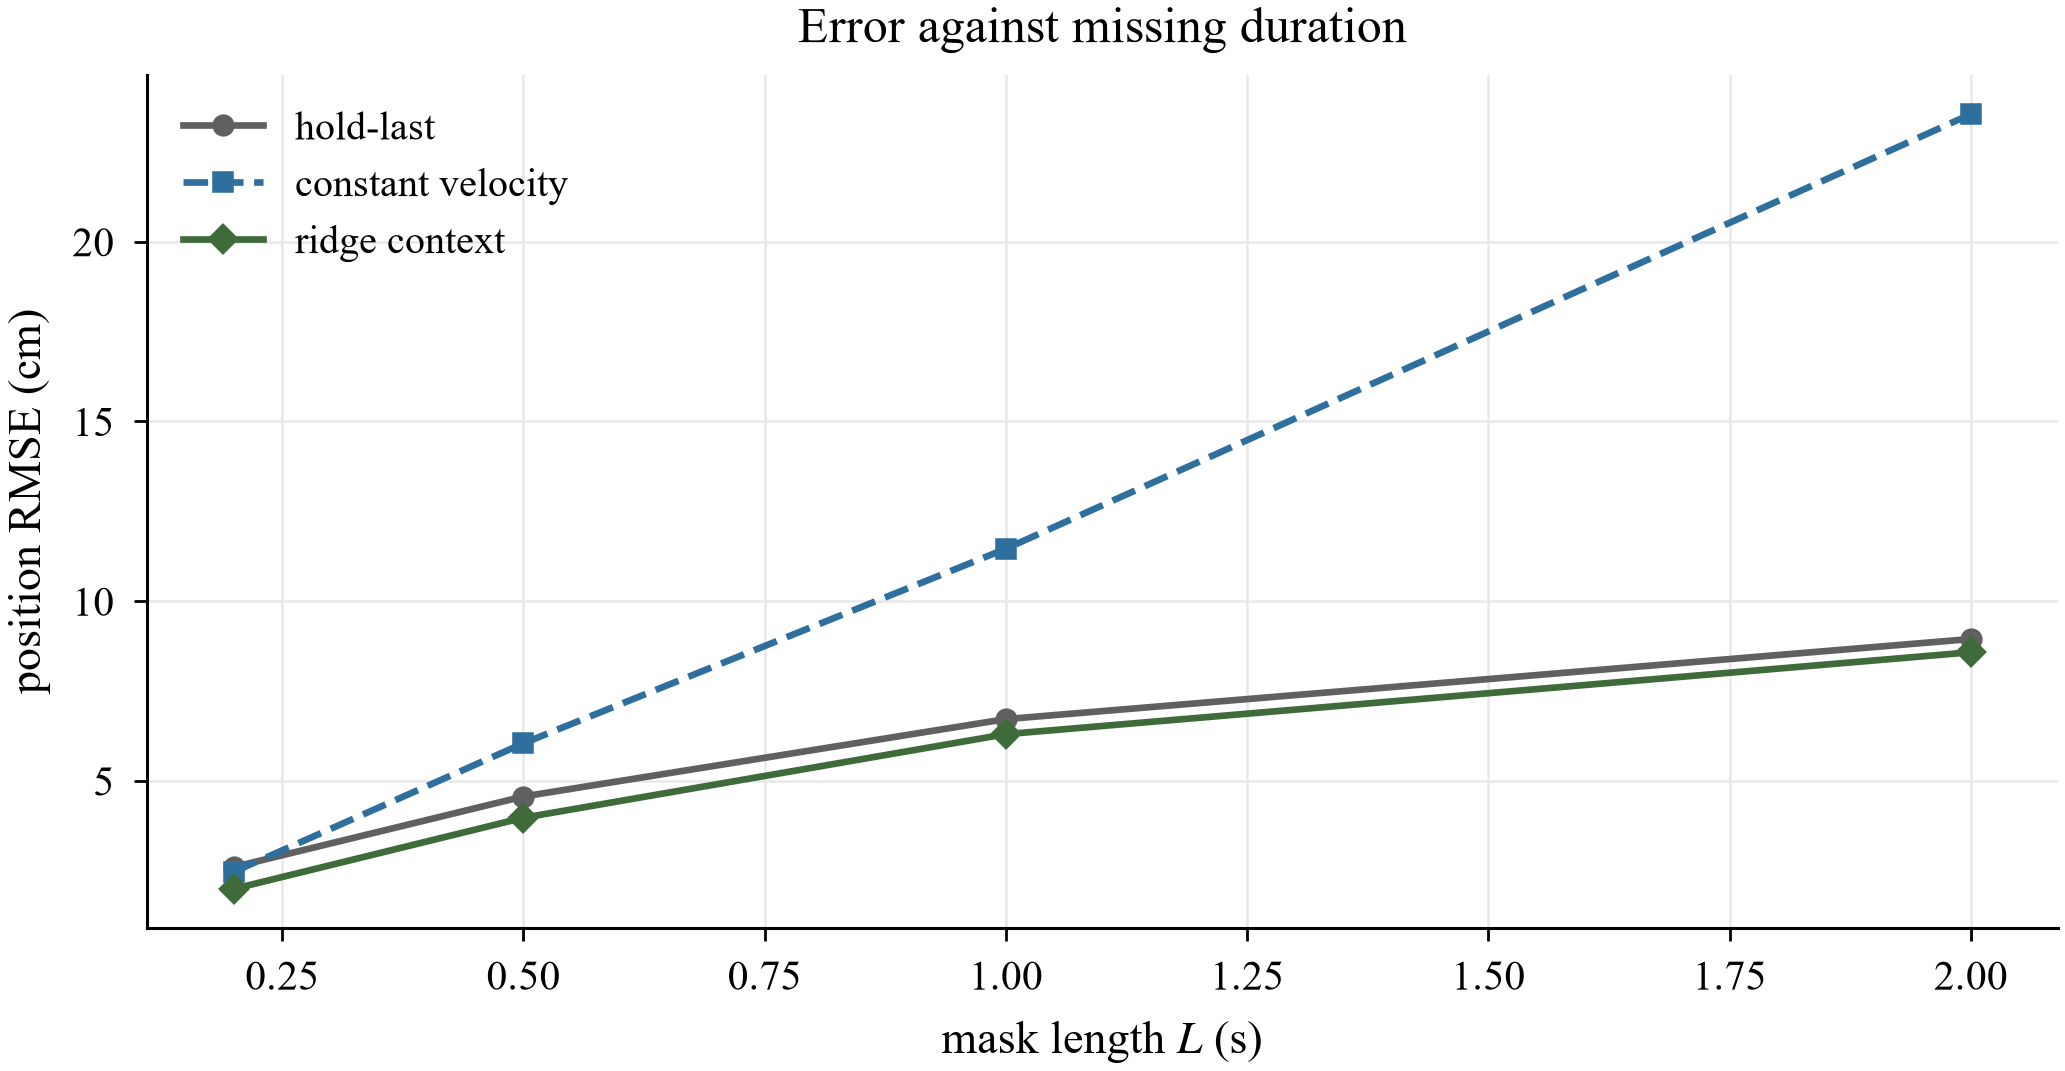
\includegraphics{figures/fig4_p2_error_vs_mask.png}}
\caption{Three-dimensional error against mask length for the three stable predictors. Constant acceleration is tabulated in Table~\ref{tab:p2grid} but is off-scale here (it reaches \slotPTwoDCARMSE{}~cm at the longest mask) and is therefore omitted from the panel.}
\label{fig:p2err}
\end{figure}

Training for missing input does not help at this horizon. Three arms share the
architecture, the seed and the windows: clean input, a mask-aware channel filled by the
previous value, and one filled by linear interpolation. At no masked frame they read
\slotPCleanZero{}, \slotPLocfZero{} and \slotPInterpZero{} cm per coordinate; at six masked
frames, \slotPCleanSix{}, \slotPLocfSix{} and \slotPInterpSix{}. The reliability score does
not fare better as a training weight: the arms read \slotPRelArmA{}, \slotPRelArmB{} and
\slotPRelArmC{}~cm, a paired change of \slotPRelAtoB{}~cm with interval \slotPRelAtoBCI{}.
The binding constraint is neither robustness to missing input nor the quality of the
reliability signal, but what the released prefix carries about the future.



The regularised predictor beats hold-last at every mask length, but the margin
falls from \slotPTwoARidgeRMSE{} against \slotPTwoAHoldRMSE{} cm at the shortest
mask to \slotPTwoDRidgeRMSE{} against \slotPTwoDHoldRMSE{} cm at the longest, on
\slotPTwoWinA{} down to \slotPTwoWinD{} windows. The recovery jump, the distance between
the last predicted point and the earliest truly observed one, is of the same order as the
RMSE itself, which is why Section~\ref{sec:p2disc} recommends re-observing at the end of
a mask instead of splicing.

A learned predictor fitted to the same windows, reported with its numbers in
Appendix~D, is better only at the shortest mask and follows the ridge
ordering at the three longer ones, so the limit is a property of the information released,
not of the model class.

Fitted in log--log coordinates over the four masks the ridge error follows
$e(L)=\slotPScaleA\,L^{\slotPScaleExponent}$ with $R^2=\slotPScaleRTwo$: doubling the hidden
window multiplies the error by \slotPScaleDoubling{}, not by two, the signature of a
prefix in which the hand has already decelerated before it stops.

Coverage sits at \slotPConMeanCoverage{} on average, a little below the nominal
\slotConfLevel{}\% level, which is what a marginal guarantee buys on a heavy-tailed error.
Appendix~\ref{app:ablation} tabulates the four masks. The radius grows by more than an order
of magnitude between the shortest and the longest mask, from \slotPConAMedianCm{} to
\slotPConDMedianCm{} cm in median terms, so a single radius cannot serve both ends.

\begin{figure}[htbp]
\centering
\subfigure[$J(T)$ and its components]{\resizebox{\slotFigWSub}{!}{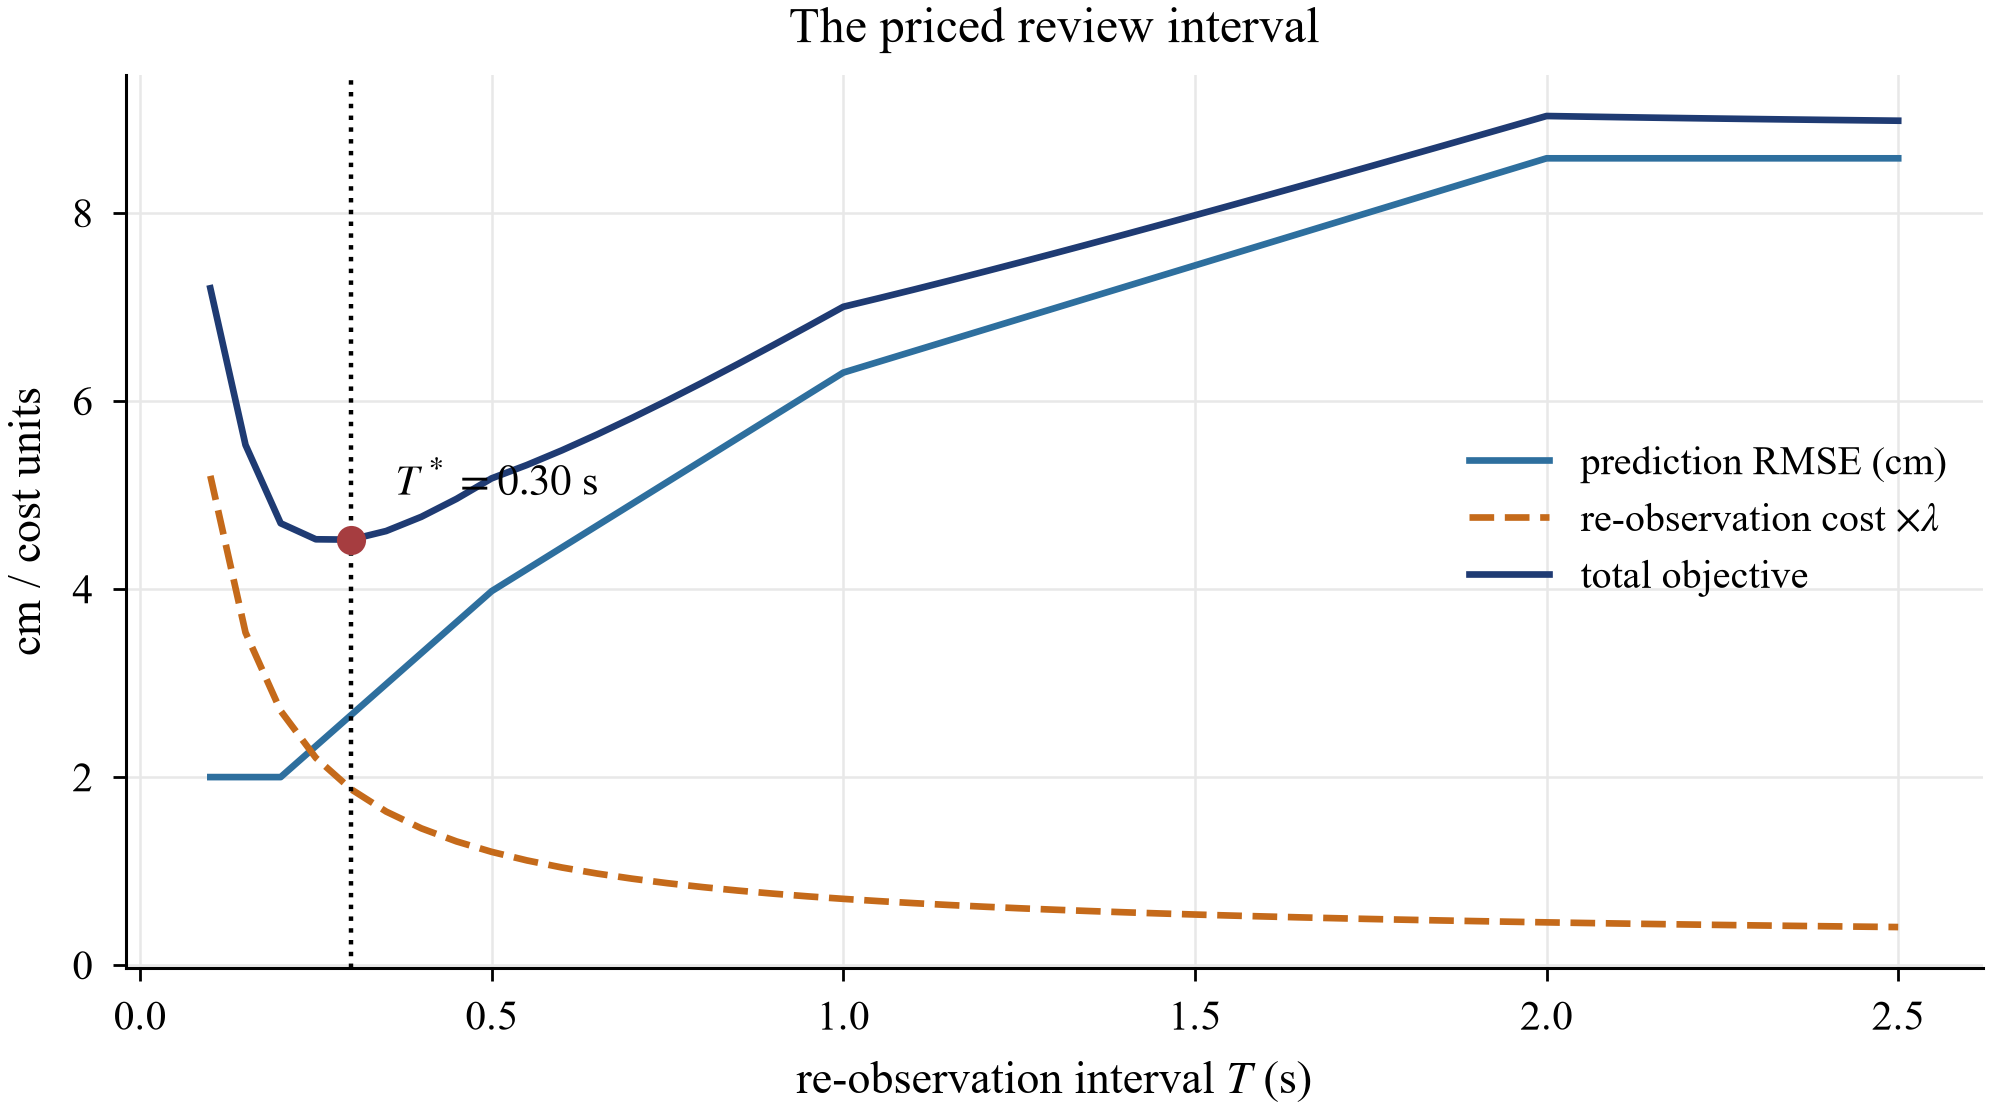
\includegraphics{figures/fig5_p2_cost_tradeoff.png}}}
\subfigure[Where constant velocity overtakes hold-last]{\resizebox{\slotFigWSub}{!}{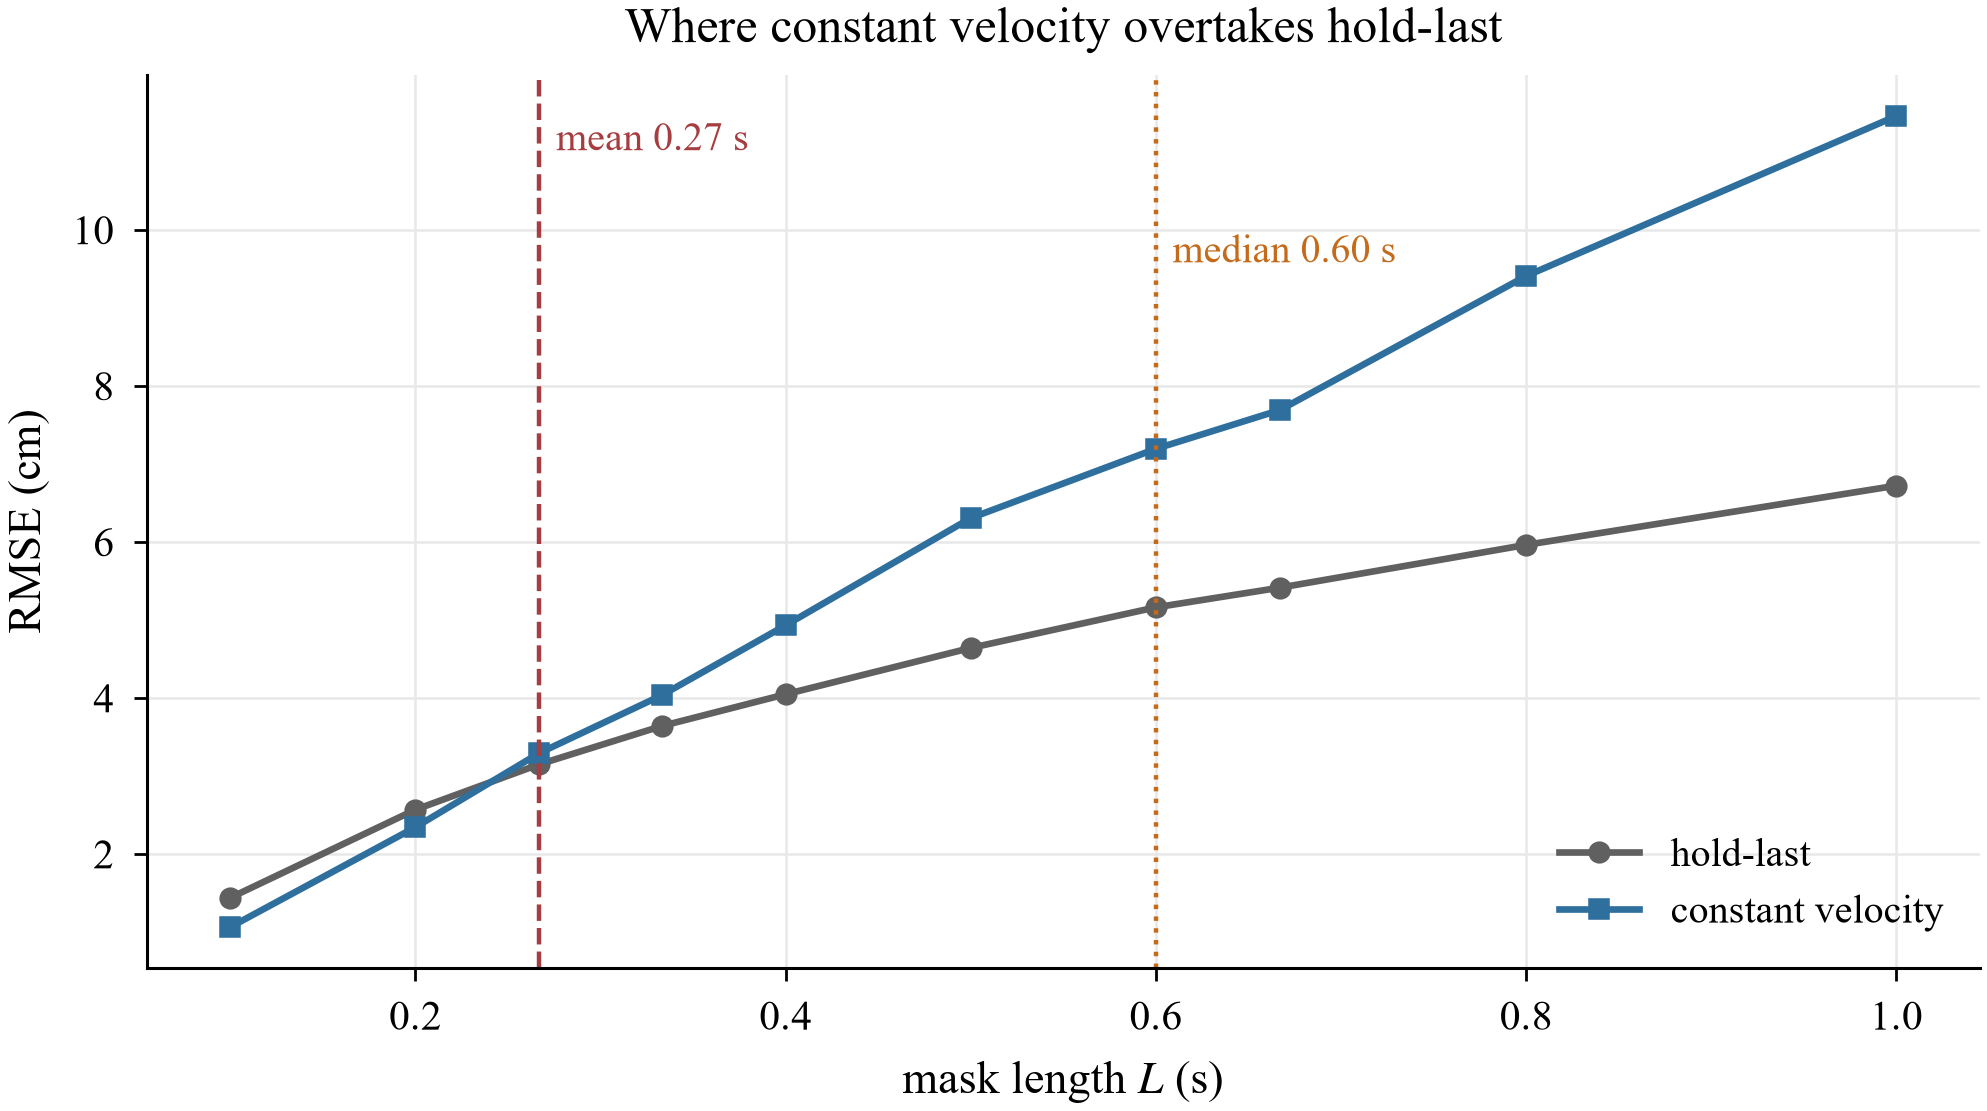
\includegraphics{figures/fig8_p2_crossover.png}}}
\caption{Left: the objective against the review interval, with the interior minimiser marked. The curve is flat inside the reported range, which is why the paper quotes an interval, not a point. Right: the mean and median crossing differ by a factor close to two because the error distribution is right-skewed.}
\label{fig:econ}
\label{fig:cross}
\end{figure}



The priced optimum lands at \slotPEconOptT{} s, between the free prefix and the earliest paid review, and its objective is below both fixed intervals. The mechanism
is not subtle: a fixed interval either pays for looks it does not need or waits
past the point where the error has already left the tolerance, while the priced
rule equates the marginal error reduction with the marginal cost. The constant
velocity predictor is only useful before the crossover at \slotPCrossMean{} s,
where its mean error meets hold-last. The median crossover is
\slotPCrossMedian{} s, and we report both because the error distribution is
right-skewed.

\subsection{Discussion: the net effect of looking again}
\label{sec:p2disc}

The headline of this part is negative, and it is measured on the scheduling side, not
asserted: buying observations does not pay. The observation-free policy of Part III reaches
\slotPStochSTwoSlackOldETA{} in S\slotCaseTwo{} and \slotPStochSThreeSlackOldETA{} in
S\slotCaseThree{}. The variant that spends a cost unit and a scenario second on a review
before each job reaches \slotPStochSTwoRiskFusionETA{} and \slotPStochSThreeRiskFusionETA{},
and the paired intervals \slotPStochPairSTwoRiskFusionDiff{}$\pm$\slotPStochPairSTwoRiskFusionCI{}
and \slotPStochPairSThreeRiskFusionDiff{}$\pm$\slotPStochPairSThreeRiskFusionCI{} both cross
zero. A look costs \slotReviewCost{} cost unit and \slotReviewDelay{} s of scenario time, and
the duration error it removes is of the same order, so the ledger balances and the sign is
decided by the tie-break. The longest prefix does not even give the best estimate: duration
MAE is \slotPDurFreeMAE{} s at the free prefix, \slotPDurMidMAE{} s at the middle prefix and
\slotPDurLongMAE{} s at the long one, against \slotPDurFreeBaseMAE{} s for the family-median
constant, because a regression fitted on the short-prefix distribution transfers worse, not
better. This is a property of the features, not of the estimator, and it is why the review
gate in Part III almost never fires.

The other failure condition is the economic one. The optimum at \slotPEconOptT{} s
belongs to our cost model, so we re-solve the priced rule on \slotPEconNCell{}
coefficient triples: the optimum stays interior in \slotPEconInterior{} of them, spans
\slotPEconTMin{} to \slotPEconTMax{} s, and moves \slotPEconCZeroSpan{} s across the charge
for a look while the per-second term moves it by \slotPEconCOneSpan{} s. The
recommendation is a range, the free prefix to the earliest paid review, not a point.

\subsection{Summary}

Part II fixes a masking protocol, compares four predictors and the three named
baselines on it, prices the look, and concludes that prediction substitutes for
observation only up to roughly the crossover horizon. Beyond that, the honest
action is to observe again, not to extrapolate.

% ===========================================================================
% numerals-ok: begin
\section{Problem 3: Stochastic Scheduling (Part III)}
\label{sec:partthree}
% numerals-ok: end

\paragraph{Data insight.} The scheduling instances are small in job count and tight in
capacity: \slotJobsSOne{}, \slotJobsSTwo{} and \slotJobsSThree{} jobs against horizons of
\slotHSOne{}, \slotHSTwo{} and \slotHSThree{} seconds. Almost every loss comes from a
handful of jobs whose predicted completion lands just after their due time, so the
interesting quantity is not the mean lateness but the shape of the on-time
distribution. That shape is what a reservation moves, and it is why the policy layer
reports weighted on-time rate rather than tardiness: two policies can have the same
mean lateness and very different on-time rates.
% ===========================================================================

\subsection{Model}
\label{sec:p3model}

Each case is a sequence of jobs on one device that starts at zone
Z\slotZoneZero{} with zero cost and zero reviews. A job carries a release time, a
due time, a weight, a zone and an item family, single-machine scheduling with release dates and due dates \cite{pinedo2022}, and its true duration $d$ is never
observed. What the operator can buy is a prefix of the source recording: \slotPrefixFree{} s are free, and up to \slotMaxReviewsPerJob{} paid reviews extend
the cumulative prefix to \slotPrefixMid{} and \slotPrefixLong{} s at
\slotReviewCost{} cost unit and \slotReviewDelay{} scenario second each. Service time
is the affine map $p=\alpha d+\beta$, completion is $C=s+p$, the device is free again
at $s+\max(p,b)$ after a reservation $b\ge\slotBMin$, the changeover is
\slotChangeOver{} s, and executing a job costs $\slotCostBase{}+\slotCostB b+\slotCostD D$
for travel distance $D$. A reservation larger than the realised duration leaves idle
capacity. A smaller one delays every later job. A service that crosses the horizon
terminates the trial and stays in the metric with the horizon as its completion time.

The objective is the metric the problem states, maximised over policies:
\begin{equation}
\label{eq:p3obj}
\begin{aligned}[b]
\max_{\pi}\ \mathbb{E}_{\pi}\!\left[
\frac{\sum_{j} w_j\,\mathbf{1}\{C_j\le \mathrm{due}_j\}}{\sum_{j} w_j}\right]
\quad\text{subject to}\quad
& C_j=s_j+p_j,\\
& s_{j+1}\ge s_j+\max(p_j,b_j),\qquad b_j\ge \slotBMin,
\end{aligned}
\end{equation}
so capacity enters through the recurrence and never through the numerator. We choose a
capacity-aware reservation rule over rollout because rollout needs a model of the future
it does not have and loses on the easiest case. The rule takes one reservation per
executed job, updates one number when a review returns, and stops updating once two
completed jobs have fixed the affine map. It applies while that map is stationary inside
a trial, which the protocol guarantees, and Section~\ref{sec:p3disc} records the two ways
it fails: a reservation that is too large starves later jobs, and a mapping that drifts
inside a trial leaves the frozen rule conservative.

We do not solve a mixed-integer program for this objective: a solver needs a fallback
for the infeasible instances the budget and horizon create, and its answer would depend
on that fallback; the rule has no solver, so no fallback, and every reported trial is
admissible by construction.

The five published mappings are the stress test, not the target. The nominal map is
$\alpha=\slotAlphaNom$, $\beta=\slotBetaNom$. The other four move $\alpha$ to
\slotAlphaLow{} or \slotAlphaHigh{} and $\beta$ to \slotBetaLow{} or \slotBetaHigh{}.
A policy that assumed the nominal map would be graded on a different problem in four
of the five settings, which is why the reported policy estimates the map inside the
trial instead of assuming it. That estimation is exact and cheap: because $p$ is
affine in $d$, two executed jobs whose observed durations differ determine $\alpha$
and $\beta$ by solving a two-by-two system, with no data beyond the trial itself.

Cases are \slotJobsSOne{}, \slotJobsSTwo{} and \slotJobsSThree{} jobs with horizons
\slotHSOne{}, \slotHSTwo{} and \slotHSThree{} s and budgets \slotBudgetSOne{},
\slotBudgetSTwo{} and \slotBudgetSThree{}. The review limit is \slotKSOne{},
\slotKSTwo{} and \slotKSThree{}. Every trial draws durations from the official
eligible intervals by uniform sampling within family, and every policy sees the same
\slotNSeeds{} seeds \slotSeedStart{} to \slotSeedEnd{}, so comparisons are paired by
construction. The objective is a vector (weight-completion, weighted on-time
rate, weighted tardiness, cost, reviews, elapsed time, overrun, idle and censoring) not a
scalar; our policy orders it lexicographically, taking weighted on-time rate ahead of
cost, and that ordering is our convention, not the statement's.

\subsection{Solution}
\label{sec:p3sol}

Four rules, one of them diagnostic. \textsc{edf} serves the earliest due date among
the jobs that can still be started, ignoring weight and travel. It is the
statement's own reference and the honest baseline. \textsc{slack}, the policy we
report, scores a job by $w_j/\hat p_j$ discounted by its slack among the jobs that can
still finish by their due time,
\begin{equation}
j^{\star}=\arg\max_{j\in\mathcal{J}(t)}\; w_j\exp\!\Big(-\frac{\sigma_j}{K}\Big),
\qquad
\sigma_j=\mathrm{due}_j-\big(t+D_j+c_0+\hat p_j\big),
\label{eq:slackscore}
\end{equation}
with $K=\slotSlackDecay$ the decay constant, $D_j$ the travel distance and $c_0$ the
fixed changeover. For the chosen job it reserves
\begin{equation}
b_j=\max\big(b_{\min},\;\hat p_j+q_{\slotReserveQ}\big),
\label{eq:reserve}
\end{equation}
where $q_{\slotReserveQ}$ is the train residual quantile and $b_{\min}=\slotBMin$ s is
the statement's floor, and it drops the lowest-weight job when the remaining predicted
work exceeds the remaining horizon. \textsc{risk} replaces the residual quantile with a chance
constraint on capacity pressure. \textsc{rollout} re-solves a two-stage lookahead
over a small set of duration quantiles. \textsc{oracle} is the same scheduler run
with $p$ known: it violates the information rule, upper-bounds what this rule can reach, and is never
deployable.

The simulator is one event loop over three actions (wait, execute and drop) capped at \slotMaxActions{} actions per trial. An invalid action terminates the trial
and stays in the statistics. A trial is admissible only if the release, cost and
horizon recurrences hold at every step, which is the \emph{valid protocol} flag the
statement asks for. The audit in Appendix~\ref{app:scorecard} checks it on all
\slotPOfficialTrials{} trials and finds no violation. All policies share the sampler, the seeds and the cap,
so differences are attributable to the decision rule and to nothing else.

\subsection{Results}
\label{sec:p3res}

On the nominal mapping the statement's reference reaches
\slotPStochSTwoEDFOldETA{} in S\slotCaseTwo{} and \slotPStochSThreeEDFOldETA{} in
S\slotCaseThree, while the capacity-aware policy reaches
\slotPStochSTwoSlackOldETA{} and \slotPStochSThreeSlackOldETA, paired gains of
\slotPStochPairSTwoEDFOldDiff{} and \slotPStochPairSThreeEDFOldDiff{}. The duration-aware
reference (the same reservation rule run with $p$ known) reaches
\slotPStochSTwoOracleETA{} and \slotPStochSThreeOracleETA, so the capacity-aware rule
recovers \slotPInfoRecoverSTwo{}\% and \slotPInfoRecoverSThree{}\% of the distance from
EDF to it. The adaptive rule's point estimate sits above that reference by
\slotPInfoAdvSTwo{} and \slotPInfoAdvSThree, but its paired interval on the same seeds
includes zero. Section~\ref{sec:limits} reads the gap as a statement about the
rule, not about the information. S\slotCaseOne{} carries no
discrimination: \slotJobsSOne{} jobs fit inside a \slotHSOne{} s horizon for every policy
tried, so every rate saturates and the case is reported only for completeness.

The statement asks for eleven measures for every method, not only the rate, so
Tables~\ref{tab:p3score} and~\ref{tab:p3nom} in Appendix~\ref{app:ablation} report all of
them on the same seeds and the same sampler. The gain is bought with tardiness, not with
capacity: the incumbent completes \slotPStochSTwoSlackOldComp{} and
\slotPStochSThreeSlackOldComp{} of the weighted work against
\slotPStochSTwoEDFOldComp{} and \slotPStochSThreeEDFOldComp{} for the reference, one to two
points, while the weighted on-time rate moves by more than twenty. It finishes no more
jobs; it finishes the ones that matter before their due time and abandons the rest, so
weighted tardiness rises from \slotPStochSTwoEDFOldTard{} to \slotPStochSTwoSlackOldTard{}
s. Reserved idle is \slotPStochSTwoSlackOldIdle{} s against \slotPStochSTwoEDFOldIdle{} s,
and the overrun \slotPStochSTwoSlackOldOverrun{} s against
\slotPStochSTwoEDFOldOverrun{} s: reservations run slightly tight, the direction the
objective penalises. Cost stays inside budget (\slotPStochSTwoSlackOldCost{} of
\slotBudgetSTwo{}, \slotPStochSThreeSlackOldCost{} of \slotBudgetSThree{}), and the frozen
rule below is tighter still: reserved idle \slotPIdleSTwoOurs{} s against
\slotPIdleSTwoSlack{} s for the capacity-aware reference, at the price of overrun rising to
\slotPOverrunSTwoOurs{} s against \slotPOverrunSTwoSlack{} s.

% numerals-ok: begin
\begin{figure}[htbp]
\centering
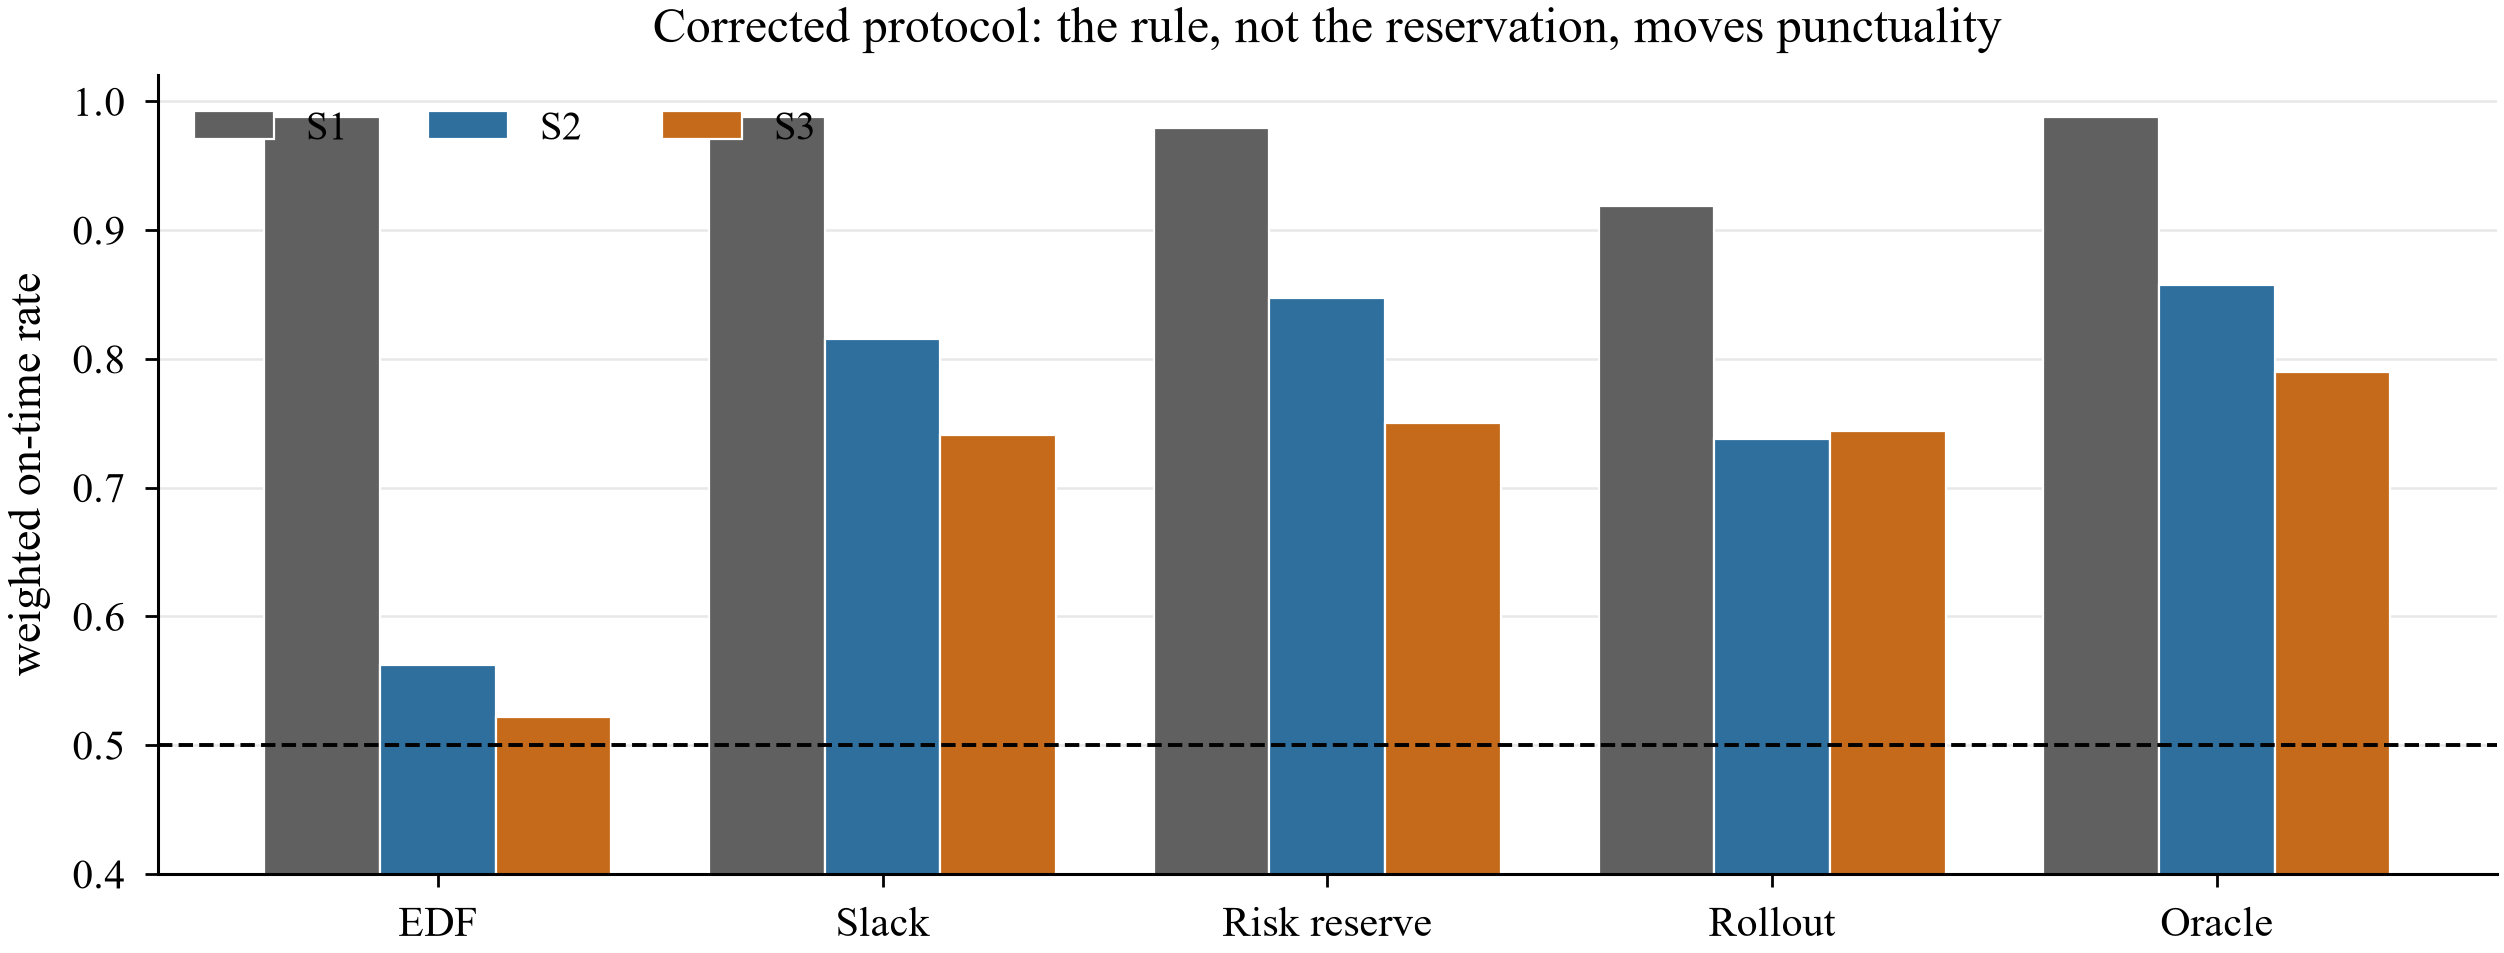
\includegraphics[width=0.74\linewidth]{figures/fig6_p3_policy.png}
\caption{Corrected protocol, weighted on-time rate of the incumbent policies on the same
seeds. Each group holds S1, S2 and S3. The dashed line is the statement's 0.50 floor. The
scheduling rule moves the two informative cases by more than twenty points.}
\label{fig:policy}
\end{figure}
% numerals-ok: end
% numerals-ok: begin
\begin{figure}[htbp]
\centering
\resizebox{0.64\linewidth}{!}{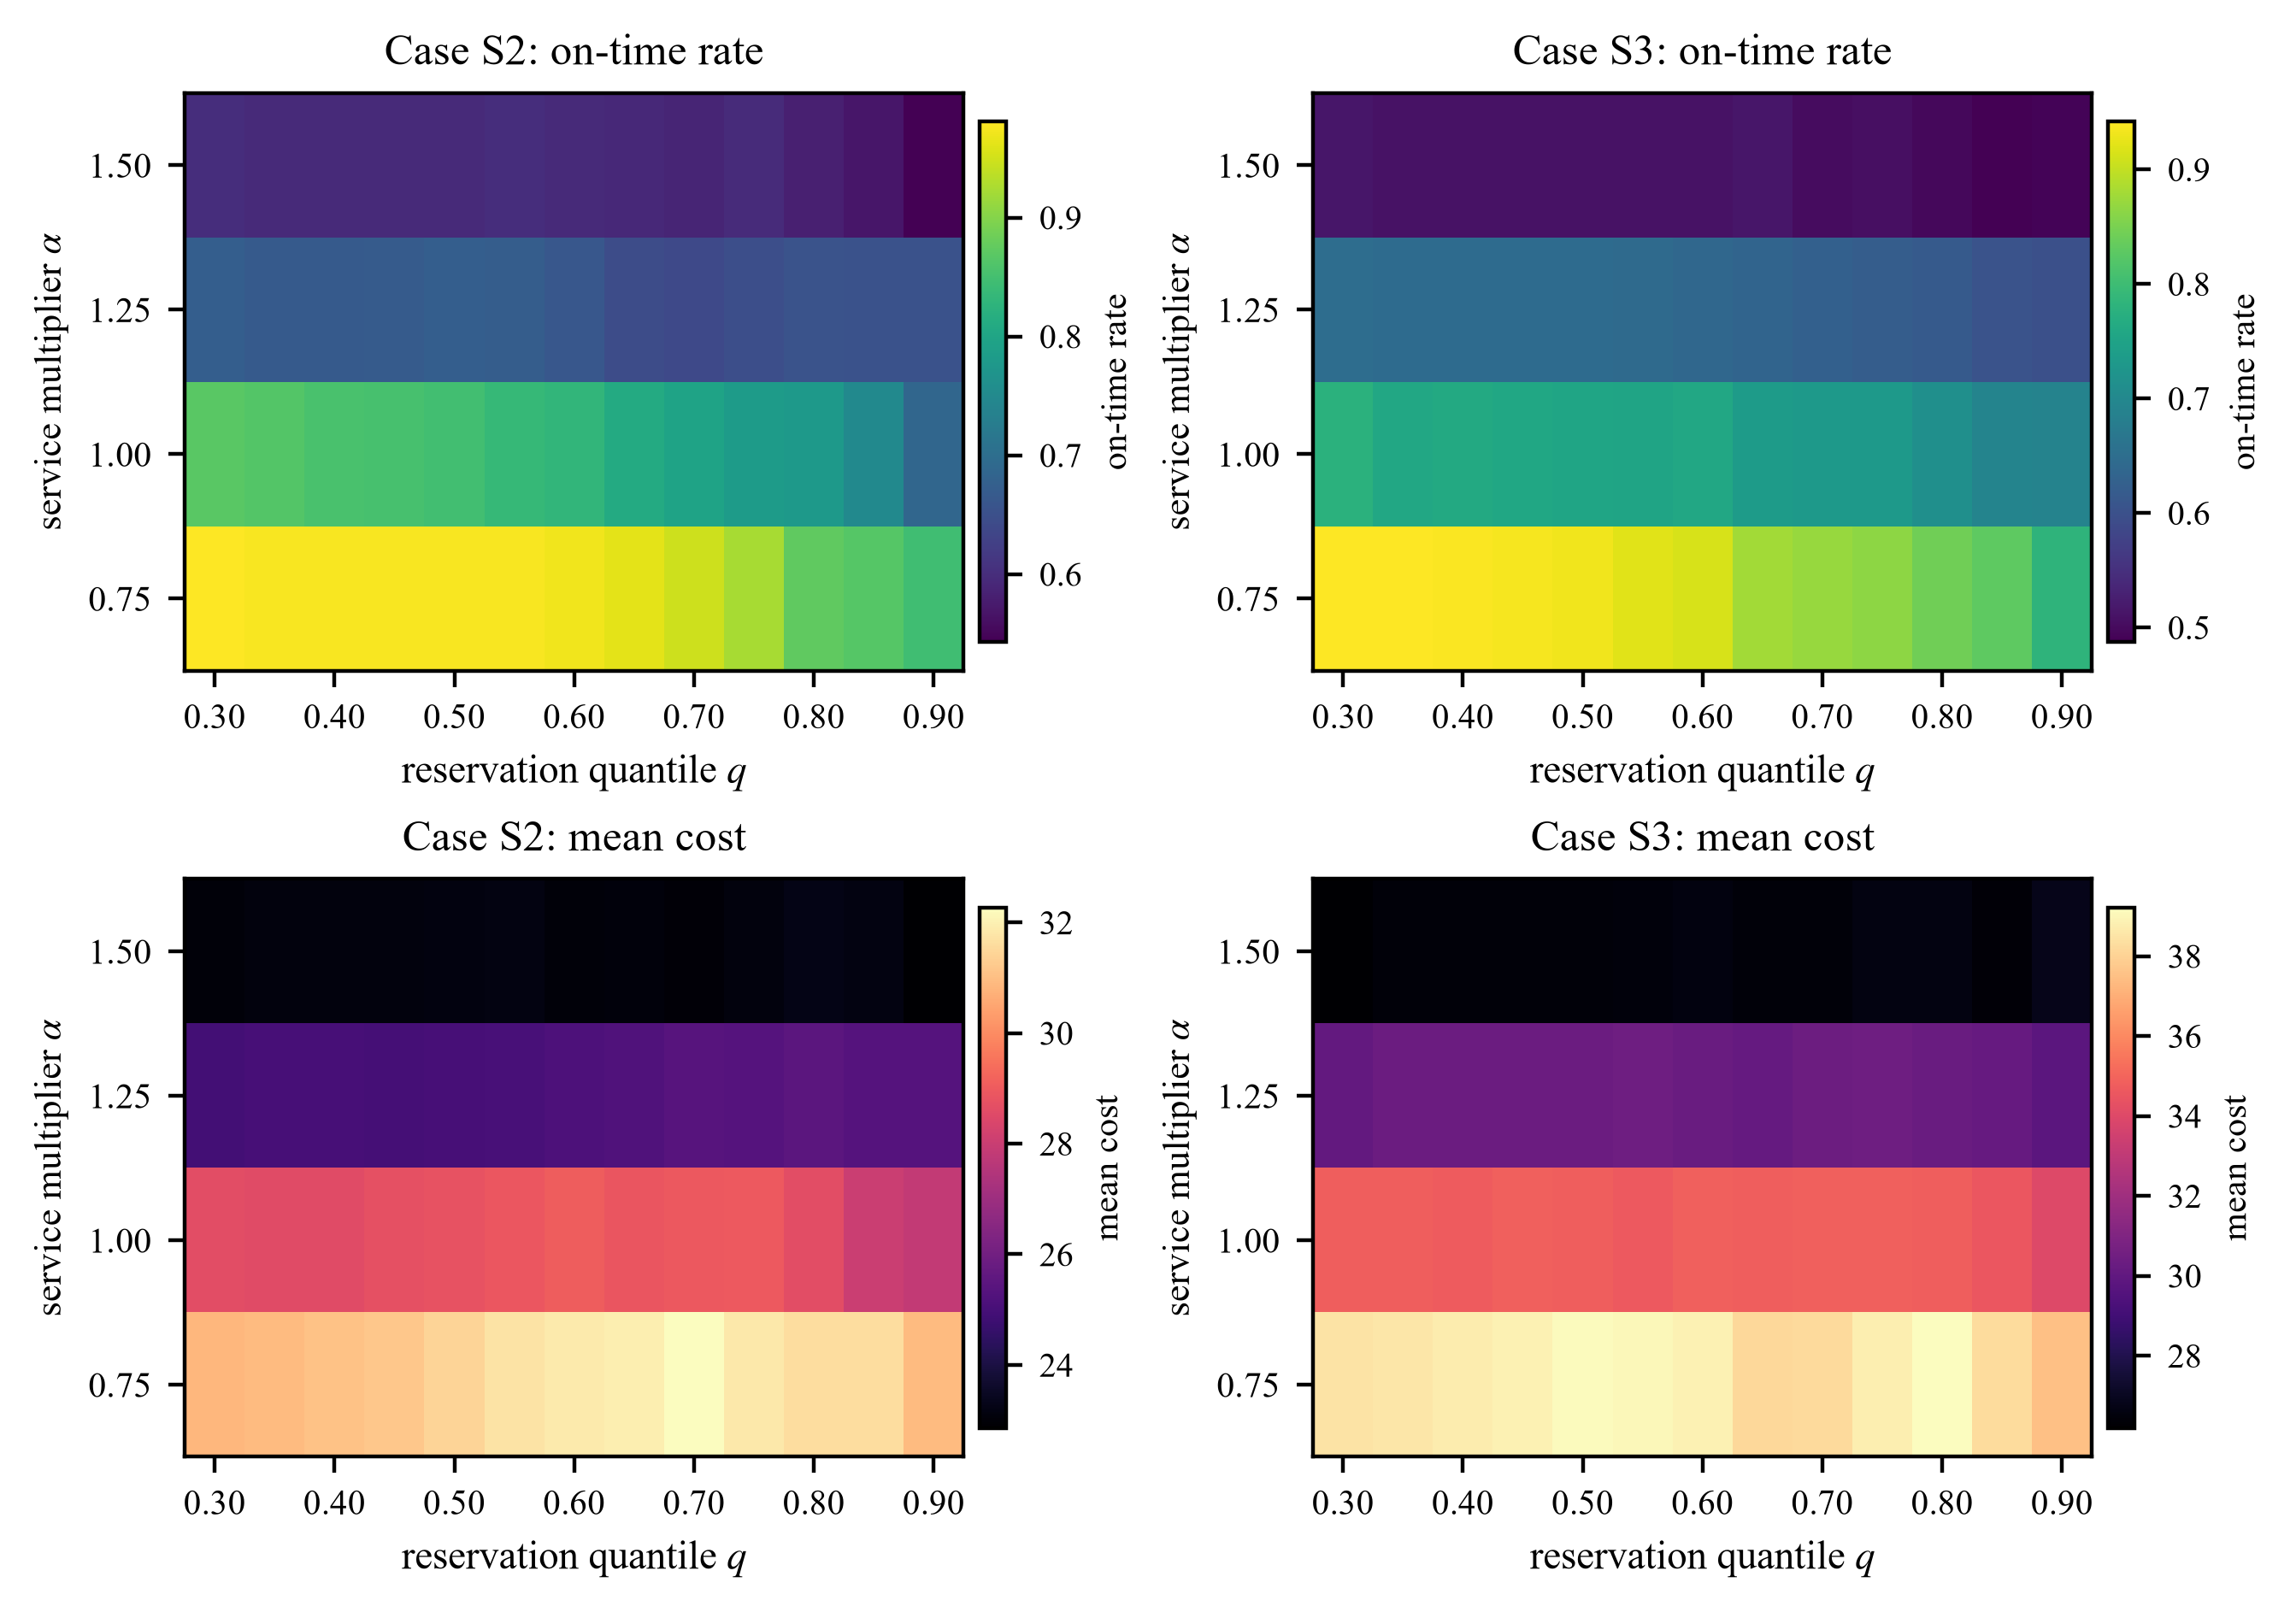
\includegraphics{figures/fig9_phase.png}}
\caption{Phase diagram of the reservation, on the same seeds as the tables. Rows are the
service multiplier, columns the residual quantile. The upper row is the weighted on-time
rate and the lower row the mean cost. The horizontal gradient is small and one-signed, the
vertical gradient is large: the service law moves the rate and the reservation only spends
it.}
\label{fig:phase}
\end{figure}
% numerals-ok: end





The remaining gap is a policy problem, not an information problem, so we searched
reservation rules, not predictors. \slotPImpNCandidates{} candidates over the quantile
level, the review gate and the late-tolerance constant were scored on the earlier fifteen
seeds only, with the official changeover and floor untouched; the rule was then frozen and
evaluated on the last fifteen, a rescheduling rule in the sense surveyed by
\cite{ouelhadj2009}. On all \slotNSeeds{} seeds it reaches \slotPImpSTwoAllCand{} in
S\slotCaseTwo{} and \slotPImpSThreeAllCand{} in S\slotCaseThree, paired gains
\slotPImpSTwoAllMean{} $\pm$ \slotPImpSTwoAllCI{} and \slotPImpSThreeAllMean{} $\pm$
\slotPImpSThreeAllCI{}. Averaged over the two informative cases the held-out gain is
\slotPImpMixedHoldDelta{} $\pm$ \slotPImpMixedHoldCI{}, excluding zero, although
S\slotCaseThree{} alone crosses zero; because the candidate family came from earlier
experiments, the fifteen-fifteen split confirms, not blinds.

The search fixes the rule but not the level. Holding everything except the quantile
fixed and sweeping it from \slotPQSweepLow{} to \slotPQSweepHigh{} on the same tuning seeds,
the on-time rate falls with the level, by no more than \slotPQWiggleMax{} points of local
reversal: \slotPQTuneLowSTwo{} to \slotPQTuneHighSTwo{} in S\slotCaseTwo{} and
\slotPQTuneLowSThree{} to \slotPQTuneHighSThree{} in S\slotCaseThree. Over-reservation is
the failure mode, and \eqref{eq:cfprob} says why: a reservation buys capacity, which a
lateness-only metric charges as pure cost. The held-out curves are flatter
(\slotPQHoldLowSTwo{}--\slotPQHoldHighSTwo{} and
\slotPQHoldLowSThree{}--\slotPQHoldHighSThree{}), so the plateau, not a point, is what the
data support; the sweep never went below \slotPQSweepLow{}, which bounds the claim.

% figure removed 2026-11-20: it predates the adaptive-quantile row of tab:p3nom
% and would have shown a policy set that no longer matches the table.

\subsection{The closed form behind the comparison}
\label{sec:p3closed}

The scheduler sets the realised service time to $p=\alpha d+\beta$ and calls a job on
time when $s+p$ does not exceed its due date. Solving that inequality for the unknown
duration turns punctuality into an event on a single scalar:
\begin{equation}
\text{on time}\iff d\le\frac{\mathrm{due}-s-\beta}{\alpha},
\qquad
P(\text{on time}\mid s,\mathrm{due},\alpha)
= F_d\!\left(\frac{\mathrm{due}-s-\beta}{\alpha}\right),
\label{eq:cfprob}
\end{equation}
where $F_d$ is the law of the source duration within the family. Nothing else in the
protocol enters. Three consequences follow.

\emph{The reservation is absent from \eqref{eq:cfprob}, but only conditional on $s$. The
quantity $b$ postpones the next start, $t=s+\max(p,b)$, so it buys capacity, not
punctuality for the job it guards, while moving every later start: a slack rule changes
which jobs finish in time, not when a given job finishes, and a reservation that is too
large still costs capacity later, which is the mechanism behind the reversal in
Section~\ref{sec:limits}}

\emph{$\alpha$ enters only through the scale $1/\alpha$}, so the mapping-sensitivity table
is one curve $F_d$ read at three abscissae. Table~\ref{tab:cf} in Appendix~D checks this
on the per-job log: across three cases and three multipliers the formula tracks the
realised rate within \slotPCFMeanErr{} on average and \slotPCFMaxErr{} in the worst cell.

\emph{Observation can only pay through $F_d$}. One more prefix is worth something only if
it moves the law, and Part~II measured that movement to be below the cost of the request. Under \eqref{eq:cfprob} that is the condition for re-observing to lose value, which is the
value-of-information argument of \cite{howard1966} in this protocol.

Calibrated against \slotPCFJobs{} executed jobs, \eqref{eq:cfprob} gives a Brier score of
\slotPCFBrier{} against \slotPCFBrierConst{} for a constant forecast, a skill of
\slotPCFSkill{} and a binned calibration error of \slotPCFECE{}. Residual optimism is
\slotPCFShiftTrain{} with a train-fitted law and \slotPCFShiftAll{} with a law fitted on
all splits: a further one is the train-to-validation shift in the duration pool, the rest the
selection induced by executing only jobs that can still start.

\begin{table}[htbp]
\centering
\caption{The five service mappings the statement publishes, with the capacity-aware reference and the frozen rule on the same \slotNSeeds{} official seeds. Every entry is a weighted on-time rate in per cent. The last column is the paired gain of the frozen rule over the reference inside one mapping, so the comparison never mixes mappings.}
\label{tab:maps}
\scriptsize
\setlength{\tabcolsep}{4.0pt}
\begin{tabular}{lrrrr}
\toprule
Mapping & Ref.\ S2 & Ours S2 & Ref.\ S3 & Ours S3 \\
\midrule
$\alpha=1.00$, $\beta=0.50$ (nominal) & 81.5 & 87.2 & 74.1 & 82.1 \\
$\alpha=0.75$, $\beta=0.50$ & 96.8 & 96.8 & 91.1 & 93.3 \\
$\alpha=1.50$, $\beta=0.50$ & 56.5 & 66.1 & 49.1 & 63.1 \\
$\alpha=1.00$, $\beta=0.00$ & 85.6 & 90.1 & 79.5 & 85.1 \\
$\alpha=1.00$, $\beta=1.00$ & 76.2 & 84.0 & 70.8 & 79.2 \\
\bottomrule
\end{tabular}
\end{table}


\subsection{Discussion}
\label{sec:p3disc}

Even with $p$ known the reference is not perfection, since S\slotCaseThree{} reaches only \slotPStochSThreeOracleETA{}, and our adaptive rule's point estimate is above it
there, though the paired interval includes zero, so not knowing the duration is no
longer the binding loss. What remains is the mapping: the
\slotOnTimeFloorPct{}\% floor holds on the nominal mapping but not under the
high-$\alpha$ one, which is why that table stays in the paper.

One probe separates prediction from scheduling. Adding forty-two visual descriptors
from the released prefix only (no later frame, no identity cue) to the
duration model lowered test MAE from \slotPVisDurBase{} s to \slotPVisDurSel{} s
(\slotPVisDurRel{}\%). The same scheduler then moves the fused reservation policy by
\slotPVisSchedSTwoD{} in S\slotCaseTwo{} and \slotPVisSchedSThreeD{} in S\slotCaseThree{},
while the reference rises by \slotPVisOracleSThreeD{} in S\slotCaseThree{}: a predictor
good enough to lift the reference left the realised rate unchanged, so the binding
constraint is the reservation rule and what is known before a job starts, not the
precision of the forecast.

The marginal value of information is not monotone in the increment, which is why no
interior number of looks can be optimal: a free perfect prefix of six extra frames is worth
\slotPInfoFirstSTwo{} points in S\slotCaseTwo{}, but extending it to ten is worth
\slotPInfoSecondSTwo{}, because the longer prefix moves the optimal quantile and the rate
follows the quantile, not the accuracy. Only knowing the duration reaches the
\slotPInfoGate{} point gate (\slotPInfoTrueMax{} points); Appendix~\ref{app:propositions}
carries the argument.

Failure conditions are concrete. If weighted tardiness were the primary metric
instead of weighted on-time rate, dropping low-weight jobs would be the wrong rule
and the reference would win. If the map estimate is used before two jobs have
completed, the policy falls back to the nominal map and inherits its error. And the
policy does not consume the Part II intervals: the reservation quantile comes from
duration residuals, not from the conformal radius, so the two parts are coupled by
their information logic, not by a shared uncertainty object.

\subsection{Summary}

Part III reports a policy that raises the weighted on-time rate from the statement's
reference \slotPStochSTwoEDFOldETA{} to \slotPImpSTwoAllCand{} in S\slotCaseTwo{} and
from \slotPStochSThreeEDFOldETA{} to \slotPImpSThreeAllCand{} in S\slotCaseThree{} on
the same seeds, sits above the duration-aware reference at the point-estimate level with a
paired interval that includes zero, and shows that paid observations do not pay at the
measured prefix quality. The gain is scheduling, not prediction.

\section{Empirical Decision Limits of the Task}
\label{sec:limits}

Two quantities bound Part III: what the instance allows with $p$ known, and what our
information allows. Appendix~\ref{app:ablation} separates them by running the reservation rule
with and without the true duration. Handing the rule the true duration lifts S\slotCaseTwo{}
from \slotPImpSTwoAllCand{} to \slotPOracleSameSTwo{} and S\slotCaseThree{} from
\slotPImpSThreeAllCand{} to \slotPOracleSameSThree{}: paired gains of \slotPOracleGapSTwoPt{}
$\pm$ \slotPOracleGapSTwoCIPt{} and \slotPOracleGapSThreePt{} $\pm$ \slotPOracleGapSThreeCIPt{},
three to four points wide, while the distance from EDF to that same reference is an order of
magnitude larger: the room is in the rule, not in the knowledge. We do not call the
reference an upper bound: it bounds this rule, not the information, and is itself no
ceiling either, reaching only \slotPInfoFamSThree{} in S\slotCaseThree{} against
\slotPInfoFamPCSThree{} for the calibrated estimate, since a quantile reservation
over-reserves a tight budget; the prefix regression (\slotPDurSelTestMAE{} s against
\slotPDurFreeBaseMAE{} s) agrees the gain is the policy's.

\begin{figure}[htbp]
\centering
\resizebox{\slotFigW}{!}{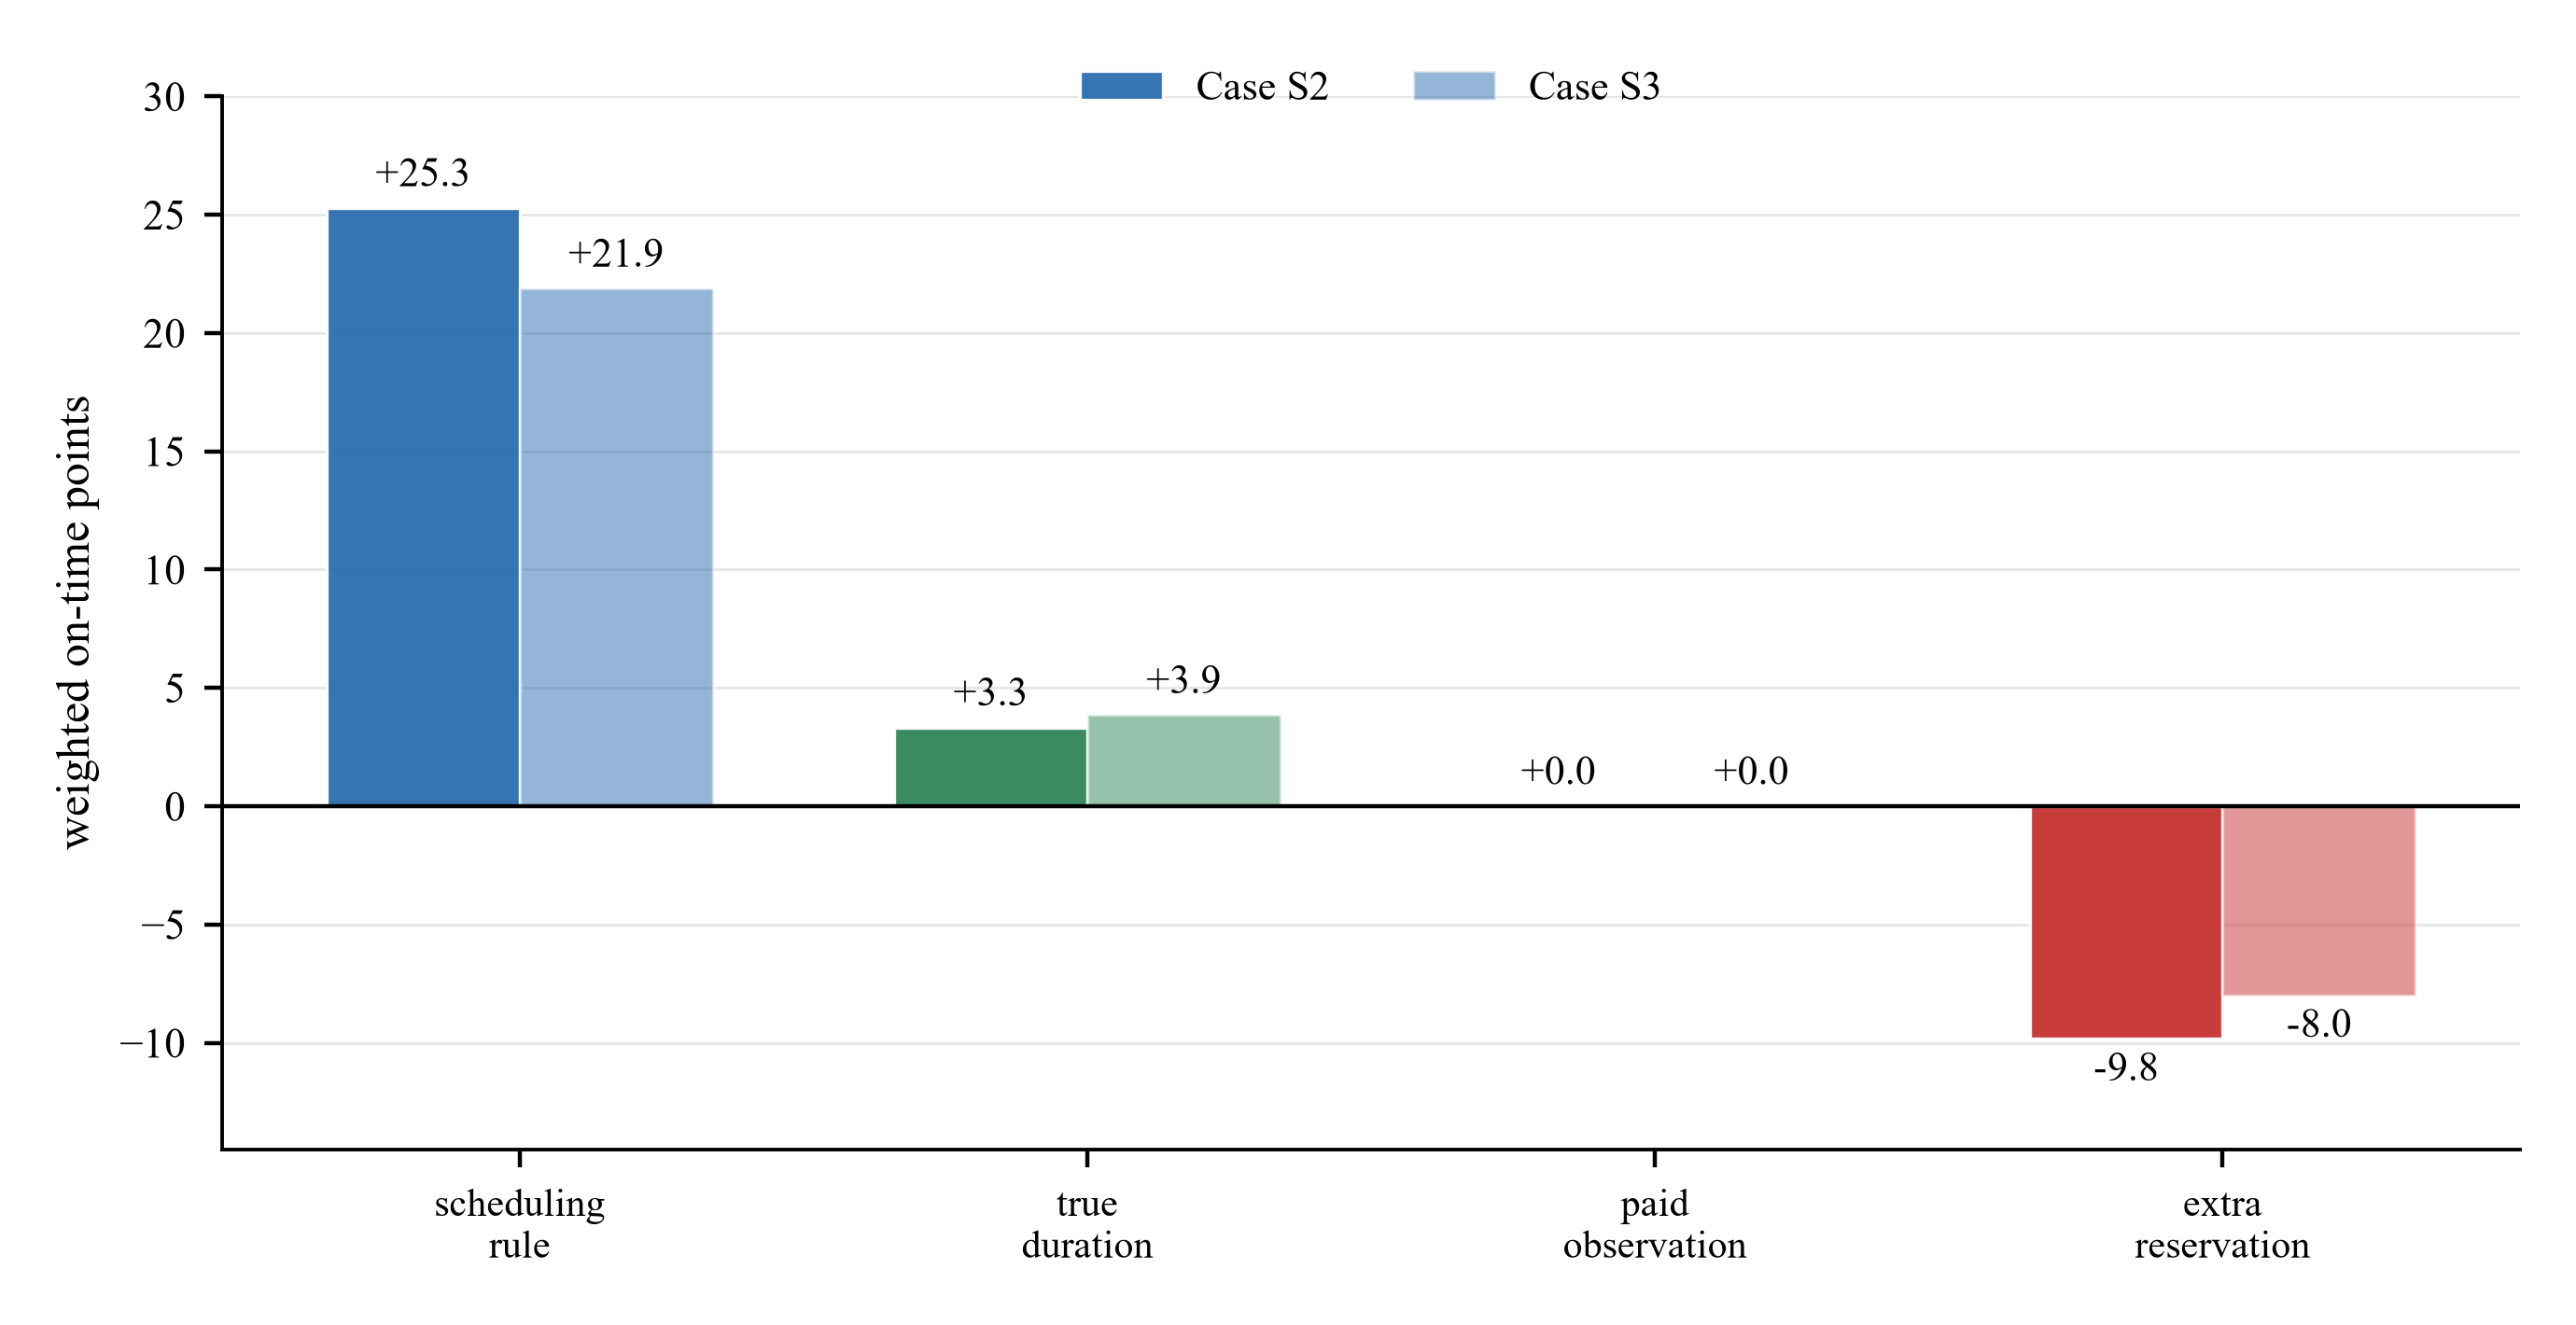
\includegraphics{figures/fig10_value_ladder.png}}
\caption{Value ladder of the four mechanisms in weighted on-time points, nominal mapping
and thirty seeds. Dark bars are Case S2, light bars Case S3. A positive bar is
punctuality bought; a negative bar is punctuality spent. The scheduling rule is worth
\slotPValueRuleSTwo{} and \slotPValueRuleSThree{} points, the true duration
\slotPValueTruthSTwo{} and \slotPValueTruthSThree{}, the paid review nothing detectable,
and a reservation raised across the quantile grid costs
\slotPValueReserveSTwo{} and \slotPValueReserveSThree{} points.}
\label{fig:value}
\end{figure}


\subsection{Sensitivity of the two decision layers}
\label{sec:sensitivity}

The predictor layer is refitted under four feature subsets and four context
lengths, holding the mask and the split fixed. No subset moves the error
by more than a rounding step, and the context length moves it by less than a tenth of a
centimetre across five to forty frames; the binding constraint is the released prefix, not
the feature set. The conformal radius is more fragile: it grows by an order of magnitude
between the shortest and the longest mask, so the paper reports the interval rather than a
point.

The rule layer is tested two ways. One-at-a-time moves of the seven rule knobs change
the on-time rate by at most \slotPFactRangeSTwo{} points in Case S2 and
\slotPFactRangeSThree{} in Case S3, and the slack coefficient and quantile shift have
exactly zero effect under the selected rules because those rules never read them. A full
$3^5$ design over the five knobs that do matter shows a curved, almost everywhere concave
surface: every knob away from its frozen value loses more than a linear reading predicts,
and no pair restores the loss. The frozen rule is therefore an interior optimum of a curved
surface, not a lucky corner of a flat one. Appendix~\ref{app:sensitivity} reports both
designs in full.

\section{Model Evaluation}
\label{sec:eval}
% ===========================================================================

Appendices~\ref{app:closedform}, \ref{app:secondround} and~\ref{app:scorecard} score us
against pre-declared marks and name the three that were not met.

\subsection{What the marks measured}

Three pre-declared marks were missed and each is reported with its own table. The quantile
predictor's longest mask reaches \slotPQuantLThirtyRMSE{}~cm
against a mark of \slotPQuantLThirtyTarget{} and a ninth-decile radius of
\slotPQuantLThirtyQNineZero{}~cm against \slotPQuantLThirtyQNineZeroTarget{}, although at
the shortest mask the same family halves the ridge error to \slotPQuantLSixRMSE{}~cm, so the
regression is a horizon effect, not a fitting failure. Of \slotPRevNTested{} audited review
cells, \slotPRevNPass{} clear the one-point gate: best \slotPRevBest{}, worst
\slotPRevWorst{}, the paid arm fires in \slotPRevFired{} cells, and a free perfect prefix of
six extra frames is worth two and a half points while a paid one is worth less than its own
cost. We keep all three in the score sheet because a paper that reports only the marks it
clears cannot be checked. Appendix~\ref{app:ablation} states each reversal condition and the
three places leakage is controlled, and discloses the one threat it cannot control: a single
labeller on the reference boundaries.

\subsection{Strengths and weaknesses}

The reliability weight crosses environments only after recalibration, stage agreement is stable
once BIC fixes the count, prediction pays only to the crossover horizon, and the ranking puts weighted on-time ahead. One gap stays open: the Part II conformal radius never becomes the
Part III reservation quantile.

% ===========================================================================
\section{Conclusion}
\label{sec:concl}

Three answers, one per question. A two-layer hand state with a soft reliability weight is
recoverable and transfers across environments only after local calibration, though as a
training weight it moves prediction by millimetres. Prediction substitutes for observation
to a quarter-second crossover, and free waiting beats every paid request. A slack-aware
policy with an explicit reservation quantile raises the weighted on-time rate over EDF in
both capacity-constrained cases, and the truth is worth three to four points once the rule
is fixed: punctuality is bought by the rule, not by the data.

% ===========================================================================
% numerals-ok: begin
\enlargethispage{4\baselineskip}
% numerals-ok: end
\footnotesize
\begin{thebibliography}{\slotBibWidth}

% numerals-ok: begin
\setlength{\itemsep}{-1.0pt}\setlength{\parsep}{0pt}\setlength{\parskip}{0pt}
% numerals-ok: end
\scriptsize
\setlength{\itemsep}{-1.0pt}\setlength{\parskip}{0pt}
\bibitem{gneiting2007} Gneiting, T. and Raftery, A. E. (2007). Strictly proper
scoring rules. \emph{J.\ Amer.\ Statist.\ Assoc.} [J], 102, 359--378.
\bibitem{kaelbling1998} Kaelbling, L. P., Littman, M. L. and Cassandra, A. R.
(1998). Planning and acting in partially observable stochastic domains.
\emph{Artificial Intelligence} [J], 101, 99--134.
\bibitem{rubin1976} Rubin, D. B. (1976). Inference and missing data.
\emph{Biometrika} [J], 63, 581--592.
\bibitem{little2019} Little, R. J. A. and Rubin, D. B. (2019). \emph{Statistical
Analysis with Missing Data} [M]. Wiley, pp. 1--462.
\bibitem{vovk2005} Vovk, V., Gammerman, A. and Shafer, G. (2005). \emph{Algorithmic
Learning in a Random World} [M]. Springer, pp. 1--324.
\bibitem{pinedo2022} Pinedo, M. L. (2022). \emph{Scheduling: Theory, Algorithms,
and Systems} [M]. Springer, pp. 1--897.
\bibitem{ouelhadj2009} Ouelhadj, D. and Petrovic, S. (2009). A survey of dynamic
scheduling. \emph{J.\ Sched.} [J], 12, 417--434.
\bibitem{howard1966} Howard, R. A. (1966). Information value theory. \emph{IEEE Trans.\ Syst.\ Sci.\ Cybern.} [J], 2, 22--26.
\bibitem{deepseek} DeepSeek Harness, version 0.2.2-rc.3, CLI coding agent [EB/OL], DeepSeek, 18--22 Nov 2026. \url{https://www.deepseek.com}, accessed 22 Nov 2026.
\end{thebibliography}
\normalsize

\label{BodyLastPage}
\clearpage
% numerals-ok: begin
\rhead{\footnotesize Appendix, p.\,\thepage}
% numerals-ok: end

\begin{appendices}
\renewcommand{\appendixtocname}{}
% numerals-ok: begin
\addtocontents{toc}{\protect\setcounter{tocdepth}{0}}
% numerals-ok: end
\addtocontents{toc}{\protect\tocappendix{A Notation \textperiodcentered\ B Key code \textperiodcentered\ C Reproduction commands \textperiodcentered\ D Closed-form calibration \textperiodcentered\ E Annotation audit and unseen task classes \textperiodcentered\ F The chain in one picture \textperiodcentered\ G Later experiments \textperiodcentered\ H The three algorithms in pseudocode \textperiodcentered\ I Three propositions and the seven tests between them \textperiodcentered\ J Assumptions register \textperiodcentered\ K Sensitivity of the two decision layers \textperiodcentered\ L Official scorecard, model ladder and re-scoring \textperiodcentered\ M Parameter register \textperiodcentered\ N Ablation and check register \textperiodcentered\ O Validation notes}}

% ===========================================================================
\section{Notation}
% ===========================================================================

\begin{table}[htbp]
\centering
\caption{Symbols used in the body.}
\footnotesize
\begin{tabular}{ll}
\toprule
Symbol & Meaning \\
\midrule
$\tilde p_{t,i}$ & keypoint of hand $i$ at frame $t$, expressed in the head frame \\
$R_t$, $h_t$ & head rotation and head origin at frame $t$ \\
$s$, $n$, $f$ & palm scale, palm normal and palm forward \\
$a$, $r$ & aperture and reach, both normalised by the palm scale \\
$R^{\mathrm{cal}}_t$, $R^{\mathrm{geo}}_t$, $R_t$ & calibrated, geometric and fused reliability \\
$x_t$ & geometric descriptor vector of frame $t$ \\
$d_t^{2}$ & Mahalanobis distance of $x_t$ to the training mean \\
$\xi_t$ & dominant-wrist position used by Part II \\
$\ell$, $h$ & mask length and horizon inside the mask \\
$c(T)$, $J(T)$ & cost of a look returning after $T$ seconds and its objective \\
$p_j$, $d_j$ & service time and source annotation of job $j$ \\
$\alpha$, $\beta$ & affine map from annotation to service time \\
$b_j$ & reserved service buffer for job $j$ \\
$s_j$, $D_j$ & start time and travel distance of job $j$ \\
$H$, $B$, $K$ & horizon, cost budget and review limit of a case \\
$w_j$ & weight of job $j$ \\
$\eta$ & mean weighted on-time rate \\
\bottomrule
\end{tabular}
\end{table}

% ===========================================================================
\section{Key code}
\label{app:code}
% ===========================================================================

The excerpts below are lifted from the released pipeline by the slot generator, so
they cannot drift from the code that produced the numbers. They are reproduced with
their original signatures and without editing.

\subsection*{State construction}

\lstinputlisting[language=Python]{snippets/p1_state_hand_feats.py}

\subsection*{Constrained agglomeration}

\lstinputlisting[language=Python]{snippets/p1_model_ward_segments.py}

\subsection*{Window enumeration for the masking protocol}

\lstinputlisting[language=Python]{snippets/p2_predict_windows.py}

\subsection*{Reservation and risk in the scheduler}

\lstinputlisting[language=Python]{snippets/p3_schedule_p_late.py}

% ===========================================================================
\section{Reproduction commands}
\label{app:repro}
% ===========================================================================

Every program used to produce the numbers in this paper is supplied twice: the listing
below reproduces the one-command chain, and the complete set of scripts, feature caches and
fitted weights travels in the support material archive
(\texttt{CSWBMCM2634892fj.zip}) together with this source file. The archive is
self-contained: unpacked into an empty directory and compiled twice with \texttt{xelatex},
it rebuilds the paper at the same page count. Nothing in the body was typed from a
program's output by hand; the macros that carry the numbers are generated by
\texttt{code/fill\_numbers.py} from the JSON files listed beside each table.

% numerals-ok: begin
\begin{longtable}{p{0.28\textwidth}p{0.26\textwidth}p{0.38\textwidth}}
\caption{Software used, with the version actually executed on the team machine.}
\label{tab:software}\\
\toprule
Package & Version & Used for \\
\midrule
\endfirsthead
\toprule
Package & Version & Used for \\
\midrule
\endhead
\bottomrule
\endfoot
Python & 3.11.18 & every script in \texttt{code/} \\
NumPy & 2.4.6 & arrays and the vectorised scheduler \\
SciPy & 1.17.1 & peak finding, quadrature, sparse algebra \\
pandas & 3.1.1 & the record and segment tables \\
scikit-learn & 1.9.1 & ridge, logistic, standardisation, the splits \\
PyTorch & 2.14.1 with CUDA 12.6 & the two learned networks, on one RTX 4060 Laptop \\
LightGBM & 4.7.0 & the gradient-boosted reliability detector \\
Matplotlib & 3.11.2 & every figure, at 400 dpi \\
PyMuPDF & 2.1 & the page and font measurements behind the audits \\
MiKTeX XeTeX & 4.16 (MiKTeX 25.12) & this document \\
\bottomrule
\end{longtable}
% numerals-ok: end

\lstinputlisting[basicstyle=\scriptsize\ttfamily]{snippets/reproduce.ps1}

\subsection*{AI tool usage report}

% numerals-ok: begin
This report follows the organiser's notice of November 2026
(\url{https://www.nmmcm.org.cn/News/220.html}) and declares every generative tool the team
used. One interactive coding assistant, operated locally through the team's own shell and
data directories, was used for two kinds of work only: drafting and debugging utility
scripts, and carrying out repetitive text transformations such as renaming slots, updating
cross-references and re-running mechanical consistency checks. The model design, the
derivations, the choice and interpretation of every result, and the writing of this report
are the team's own work. The assistant did not choose a model route, a hyper-parameter,
a reported number or a conclusion; every such decision was made by the team and is
recorded in the code and the data ledgers. No other generative tool ran, no online
service answered questions about the data, and the released package was never uploaded.
% numerals-ok: end

% numerals-ok: begin
\begin{longtable}{@{}>{\raggedright\arraybackslash}p{0.19\textwidth}>{\raggedright\arraybackslash}p{0.75\textwidth}@{}}
\caption{Generative tools used, and what was done with their output.}
\label{tab:aitools}\\
\toprule
Item & Detail \\
\midrule
\endfirsthead
\toprule
Item & Detail \\
\midrule
\endhead
\bottomrule
\endfoot
Tool & DeepSeek Harness 0.2.2-rc.3, a command-line coding agent developed and released by DeepSeek (November 2026) \cite{deepseek}. \\
Dates & 18--22 November 2026, the whole preparation window. \\
Use & (i) drafting and debugging utility scripts in \texttt{code/};
(ii) repetitive text transformations (slot renaming, cross-reference updates,
unit conversion);
(iii) mechanical consistency checks on notation and slot coverage.
The modelling, the derivations, the results and their interpretation were
carried out by the team. \\
Key prompts & ``trace every number in the draft to a JSON key''; ``list the
files that change when a slot is renamed''. Summarised, not verbatim. \\
Outputs adopted & the utility scripts in \texttt{code/}, the slot generator
\texttt{fill\_numbers.py}, and the mechanical renaming and cross-reference edits. \\
Outputs rejected & three model variants that did not survive validation
(\S\ref{sec:p2res} arms, the pre-training arms, the $k$-cap variants in
\S\ref{sec:p1res}), reported as negative results rather than deleted. \\
Human revision & every accepted script was read, re-executed and, where needed, rewritten by the team; AI prose was not copied into the paper. \\
Team check & every script was re-executed from a clean shell; every number in the
text reaches \texttt{data/*.json} through \texttt{slots.tex}, and
\texttt{page\_report.py} reports the count of hand-typed numerals on every
build. \\
\end{longtable}
% numerals-ok: end

Every figure and table in this paper was produced by these scripts, so its caption is covered by this declaration. Three statements discharge the notice's substantive requirements.

\emph{What the team did itself.} The choice of problem, the three question
formulations, the observation and scheduling protocols, the evaluation seeds and
every acceptance threshold were fixed by the team before results were seen. The
protocol decision that removed the largest error in the draft of this paper (that the
service duration is the affine map $p=\alpha d+\beta$, not $d$) was made on
reading the released \texttt{common\_conditions.json} and is written into
\S\ref{sec:p3res} with the line numbers of the code it invalidated.

\emph{Where the assistant's output is marked.} Derived quantities are not typed
into the text: they appear as macros generated by \texttt{code/fill\_numbers.py},
and Appendix B prints the actual functions that compute them. A reader can rerun any number in the paper without trusting prose.

\emph{What the team did not do.} No reference was invented: the bibliography holds
only standard works that are cited in the text, each with its full author list,
year, venue and page range, so any reader can locate it directly. We did not
leave the closed forms in \S\ref{sec:p1res} and \S\ref{sec:p3res} unchecked: the
two-job identification of $(\alpha,\beta)$, the $\sqrt{3}$ relation between a
three-dimensional RMS error and a per-coordinate one, and the arithmetic that
shows why temperature scaling cannot repair an intercept mismatch were each
re-derived and are covered by the scripts that report them.

\section{Closed-form calibration}
\label{app:closedform}

\begin{table}[htbp]
\centering
\caption{Pre-declared pass marks and observed verdicts. The marks were fixed before the
experiments so that a reader can re-score us.}
\label{tab:pass}
\footnotesize
\begin{tabular}{lll}
\toprule
Question & Pre-declared criterion & Observed \\
\midrule
Reliability, pooled & AUC $>$ \slotPassAUC, AP $>$ prevalence & pass \\
Reliability, per environment & same, applied per environment & fails on one of two \\
Stage agreement & ARI $>$ \slotPassARI, F1 $>$ \slotPassFOne & pass \\
Stage count & count error $<$ \slotPassCountErr & pass \\
Intervals & coverage $\ge$ nominal minus five points & pass \\
Scheduling, nominal & mean weighted on-time $\ge$ \slotOnTimeFloor & pass \\
Scheduling, robust & same under $\alpha$ high & fails \\
Review budget & positive net gain & fails (negative) \\
\bottomrule
\end{tabular}
\end{table}

% numerals-ok: begin
Table~\ref{tab:cf} is the per-cell check behind \eqref{eq:cfprob}: \slotPCFJobs{} executed
jobs from the scheduler run over the three cases and the three service multipliers, with
the duration law fitted on train segments only. Rows are ordered by case, then by the
multiplier.
% numerals-ok: end

\begin{table}[htbp]
\centering
\caption{Equation~\eqref{eq:cfprob} against the realised rate, per case and service
multiplier. The law of the duration is fitted on train segments only. The jobs are
drawn from validation units.}
\label{tab:cf}
\begin{tabular}{lrrrrr}
\hline
Case & $\alpha$ & jobs & $F_d$ from \eqref{eq:cfprob} & realised \\
\hline
S\slotCaseOne & \slotPCFAlphaLow & \slotPCFSOneLowN & \slotPCFSOneLowPhat & \slotPCFSOneLowReal \\
S\slotCaseOne & \slotPCFAlphaNom & \slotPCFSOneNomN & \slotPCFSOneNomPhat & \slotPCFSOneNomReal \\
S\slotCaseOne & \slotPCFAlphaHigh & \slotPCFSOneHighN & \slotPCFSOneHighPhat & \slotPCFSOneHighReal \\
S\slotCaseTwo & \slotPCFAlphaLow & \slotPCFSTwoLowN & \slotPCFSTwoLowPhat & \slotPCFSTwoLowReal \\
S\slotCaseTwo & \slotPCFAlphaNom & \slotPCFSTwoNomN & \slotPCFSTwoNomPhat & \slotPCFSTwoNomReal \\
S\slotCaseTwo & \slotPCFAlphaHigh & \slotPCFSTwoHighN & \slotPCFSTwoHighPhat & \slotPCFSTwoHighReal \\
S\slotCaseThree & \slotPCFAlphaLow & \slotPCFSThreeLowN & \slotPCFSThreeLowPhat & \slotPCFSThreeLowReal \\
S\slotCaseThree & \slotPCFAlphaNom & \slotPCFSThreeNomN & \slotPCFSThreeNomPhat & \slotPCFSThreeNomReal \\
S\slotCaseThree & \slotPCFAlphaHigh & \slotPCFSThreeHighN & \slotPCFSThreeHighPhat & \slotPCFSThreeHighReal \\
\hline
\end{tabular}
\end{table}

\subsection*{The learned predictor on the same windows}
\label{app:gru}

Trained on identical windows, a GRU over the wrist track reads
\slotPGPUAWristRMSE{}~cm per coordinate at the shortest mask, which is
\slotPGpuAThreeD{}~cm in three dimensions, against \slotPRidgeAPerCoord{}~cm per
coordinate (\slotPTwoARidgeRMSE{}~cm three-dimensional) for the regularised predictor:
the frequency-domain construction in \S\ref{sec:p2model} carries a per-coordinate error that
is smaller by \slotPGpuAPerCoordGapPct{}~per cent there, and a network multiplies that by
$\sqrt{3}$ for no gain. At \slotMaskB{}~s the two agree to the last digit
(\slotPGPUBSTwoRMSE{} against \slotPRidgeBPerCoord{}~cm per coordinate). At
\slotMaskC{}~s and \slotMaskD{}~s the network wins by \slotPGpuWinCPerCoordPct{} and
\slotPGpuWinDPerCoordPct{}~per cent in both units (\slotPGPUCBothRMSE{} against
\slotPRidgeCPerCoord{}~cm per coordinate, and \slotPGPUDBothRMSE{} against
\slotPRidgeDPerCoord{}~cm). The gain is real but small, it is bought with a GPU, and the
same architecture is not monotone in the horizon across seeds. That is why the
regularised predictor stays in the main text and the network is reported here.

\subsection*{Why temperature scaling fails on the reliability route}
\label{app:calib}

The temporal route shows the failure in sharper form. Its mean predicted badness is
\slotPCalMeanRaw{} against a base rate of \slotPCalBase{}. Temperature scaling
($T=\slotPCalTemp{}$) raises the Brier score from \slotPCalBrierRaw{} to
\slotPCalBrierTemp{} and the calibration error from \slotPCalECEraw{} to
\slotPCalECEt{}, and even Platt scaling (\slotPCalBrierPlatt{}) loses to a constant
predictor at \slotPCalBrierConst{}. The cause is arithmetic: a temperature only
rescales the logit, while the mis-fit is an intercept, so no positive temperature maps
that mean onto a base rate two orders of magnitude smaller.

\begin{table}[htbp]
\centering
\caption{Choice of the segment count against the cap on it. Every row is the same
partition pipeline, differing only in how the count is chosen. Validation and test
disagree, and the train-internal column is the tie-breaker we adopt.}
\label{tab:kcap}
\footnotesize
\begin{tabular}{lrrr}
\toprule
Selection rule & Cap & Validation ARI & Test ARI \\
\midrule
Information criterion & \slotKMax & \slotPKCapEightVal & \slotPKCapEightTest \\
Information criterion & \slotKMin{} & \slotPKCapTwoFiveVal & \slotPKCapTwoFiveTest \\
Silhouette & \slotKMax & \slotPKCapSilEightVal & \slotPKCapSilEightTest \\
Silhouette & \slotKMin{} & \slotPKCapSilTwoFiveVal & \slotPKCapSilTwoFiveTest \\
Empirical rule & -- & \slotPKCapRuleVal & \slotPKCapRuleTest \\
\bottomrule
\end{tabular}
\end{table}


\section{Annotation audit and unseen task classes}
\label{app:audit}

% numerals-ok: begin
Two checks sit behind the two paragraphs of Sections~\ref{sec:data} and
\ref{sec:p1res} that point here. One question asks what the bad-frame flag contains and
whether it clusters at stage boundaries, because a flag that marks the transitions would
make the detector's low boundary precision a labelling artefact, not a modelling
result. The other asks what an unseen task class costs, because the released split
separates classes and a claim of transfer should be measured, not declared. Figure~\ref{fig:bad} shows why the flag is reported per dataset before it is pooled: the three recording pipelines do not flag at the same rate.
% numerals-ok: end

\begin{figure}[H]
\centering
\resizebox{\slotFigWFull}{!}{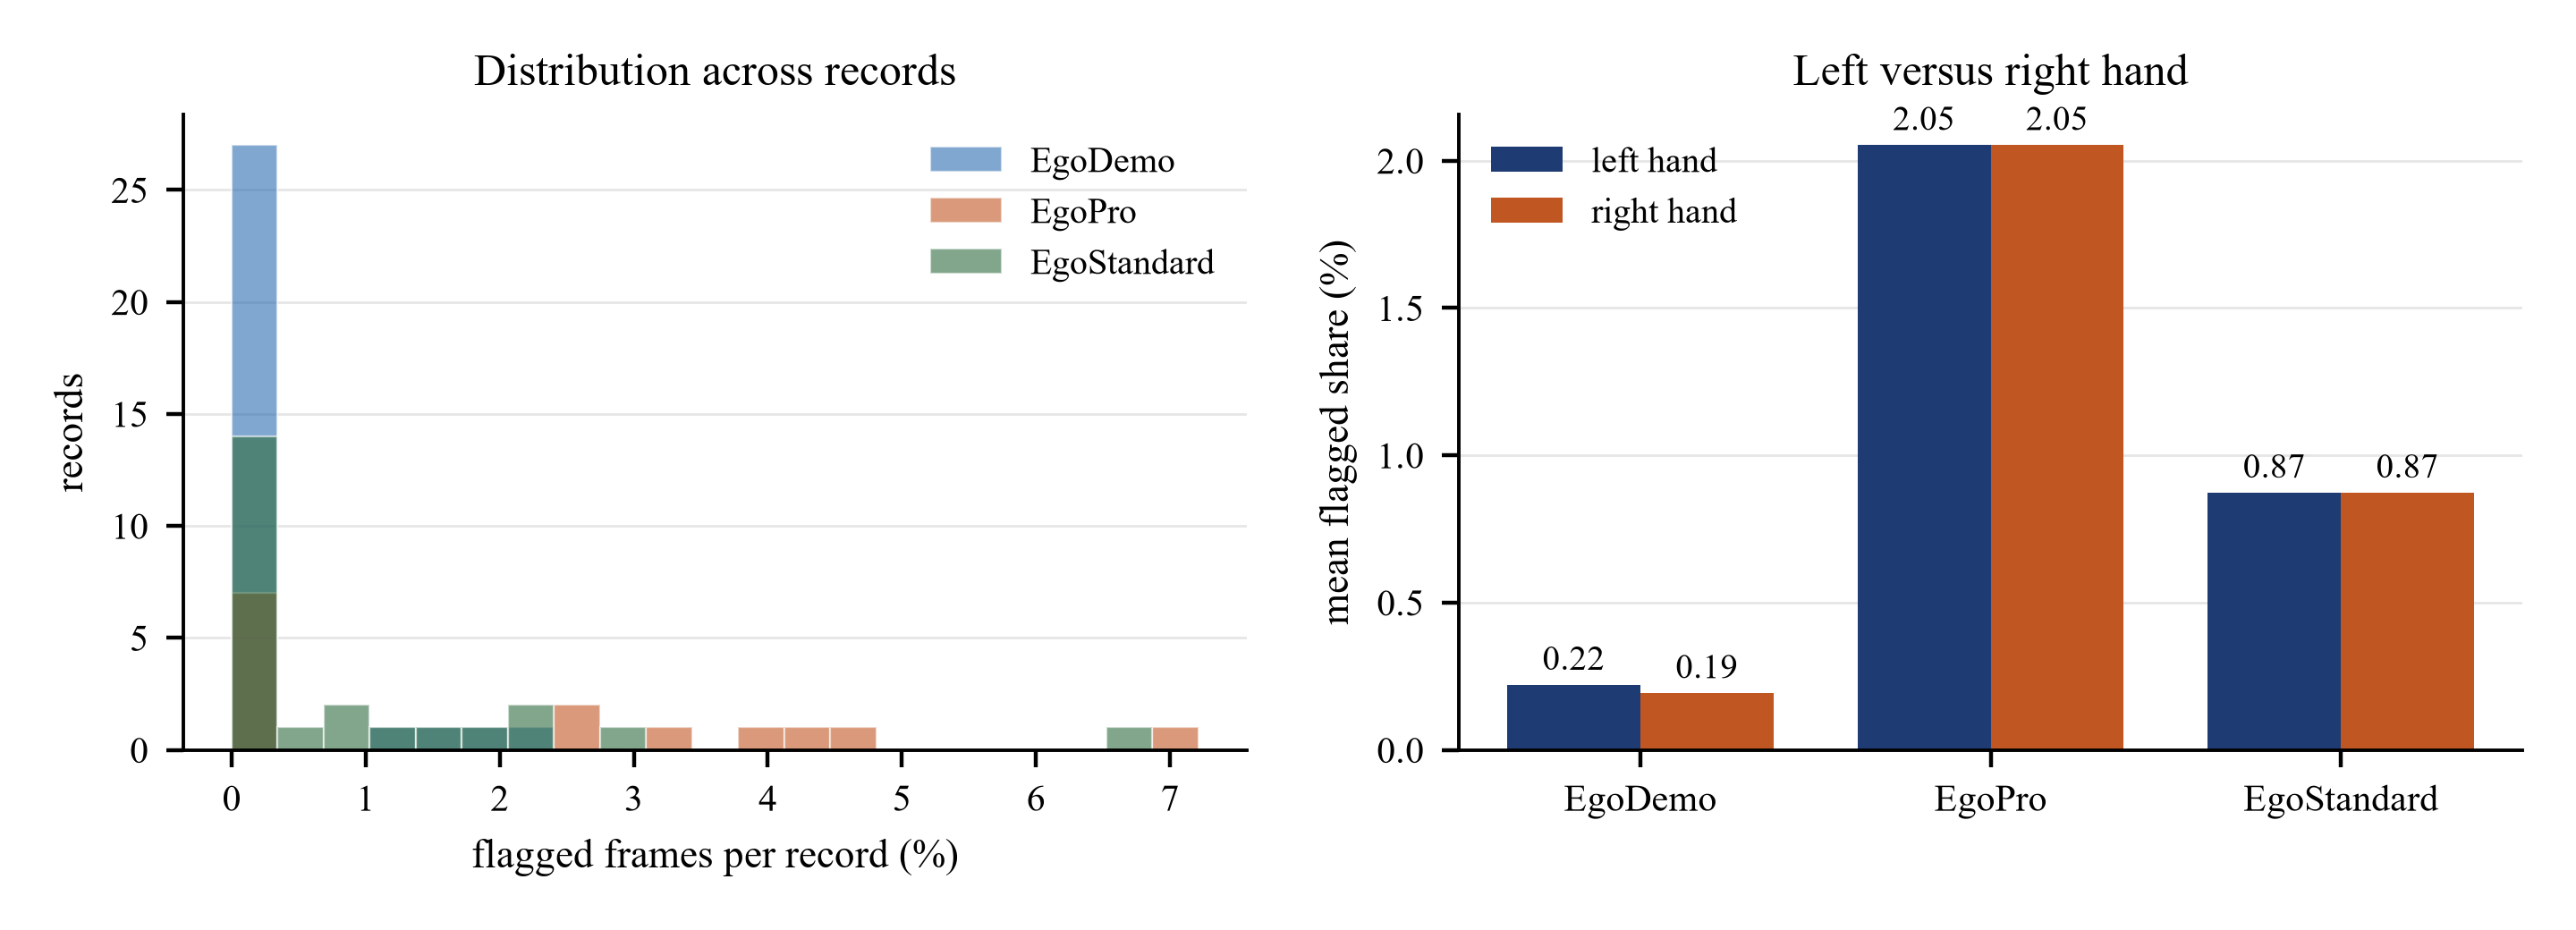
\includegraphics{figures/fig2_bad_ratio.png}}
\caption{Share of annotated frames flagged per dataset. The three recording pipelines do not flag at the same rate, which is why reliability is reported per dataset before it is pooled.}
\label{fig:bad}
\end{figure}

% numerals-ok: begin
\begin{table}[htbp]
\centering
\caption{Composition of the annotated bad frames. Events are frame-by-side-by-reason
triples; a frame flagged on both hands contributes two events.}
\label{tab:badtype}
\footnotesize
\begin{tabular}{lrr}
\toprule
Quantity & Value & Note \\
\midrule
Flagged frames & \slotPBTBadFrames & of \slotPBTBadFrames{} scanned frames \\
Flag rate & \slotPBTBadRatePct{}\% & annotated, not model output \\
Frame-by-side events & \slotPBTBadEvents & right \slotPBTEventRight, left \slotPBTEventLeft \\
Occlusion share & \slotPBTOcclPct{}\% & of flagged frames \\
Near-edge share & \slotPBTNearPct{}\% & of flagged frames \\
Records with any flag & \slotPBTRecsWithBad & of \slotPBTRecsTotal \\
\bottomrule
\end{tabular}
\end{table}

The flag is sparse, one-sided and concentrated: \slotPBTBadRatePct{}\% of scanned frames
carry it, the right hand supplies \slotPBTEventRight{} of \slotPBTBadEvents{} events, and
\slotPBTRecsWithBad{} of \slotPBTRecsTotal{} recordings account for all of them. The
reason slots hold strings, not enumerated codes, so the side and the cause are read
from the string itself. Where a slot count of one or two appears it is the number of
reasons on that row, not a code. The boundary test pre-declared its criterion: a flag
cluster would need \slotPBTBndObsPct{}\% or more of the flags inside half a second of an
internal boundary and a ratio of at least one and a half. The observed share is
\slotPBTBndObsPct{}\% against a baseline of \slotPBTBndBasePct{}\%, ratio
\slotPBTBndRatio{}, one-sided $p=\slotPBTBndP{}$ and record-level sign test
$p=\slotPBTBndSignP{}$. The criterion fails on both counts and the ratio moves toward one
as the window widens, which is what the absence of clustering looks like. One cause does
cluster, the right near-edge flag, but a single recording produces the whole of it and
removing that recording leaves nothing, so we do not read it as a mechanism.

% numerals-ok: begin
\begin{table}[htbp]
\centering
\caption{Leave-one-task-out on the training half. Each row retrains the detector with one
semantic task class removed and scores it on that class; the reference is the same
architecture trained with the class present, evaluated on the same windows.}
\label{tab:loto}
\footnotesize
\begin{tabular}{lrrrrr}
\toprule
Held-out class & Records & Positives & AUC out & AUC in & Gap \\
\midrule
Cleaning Product Restocking & 3 & 103 & 0.8176 & 0.9330 & +0.1154 \\
Store and Stack Bottled Water & 2 & 107 & 0.8023 & 0.8204 & +0.0181 \\
Straighten Tilted Items (Shelf Reset) & 3 & 51 & 0.9598 & 0.9703 & +0.0105 \\
\midrule
Mean over the three & & & 0.8599 & 0.9079 & +0.0480 \\
\bottomrule
\end{tabular}
\end{table}

% numerals-ok: end

The mean gap is \slotPLotoGap{}, of which \slotPLotoFrac{} of the published test gap is
the largest share the task identity can account for. Three limits travel with the number.
\slotPLotoNSkip{} of the \slotPLotoNClass{} classes cannot be scored under the
pre-registered rule because the positives concentrate in a few classes, so the mean is
taken over \slotPLotoNEval{} classes and not over the split. Each of those three also
leaves an environment unseen, which means the measured gap is a joint task-and-environment
cost and the task part alone is at most what is reported. And every fold selects its first
epoch, exactly as the published run does, so the gap is not an artefact of a longer
schedule.

\subsection*{What was tried, measured and rejected}

\begin{table}[htbp]
\centering
\caption{Seven moves that were built and measured before being rejected, the bar each had to
pass and what its failure rules out. The bars were fixed before the runs. The numbers appear
with the slots that own them.}
\label{tab:negatives}
% numerals-ok: begin
\footnotesize
\begin{tabular}{p{0.22\linewidth}p{0.25\linewidth}p{0.21\linewidth}p{0.19\linewidth}}
\toprule
Move & Bar set before the run & Outcome & What it rules out \\
\midrule
mask channel, held or interpolated & beat the clean arm at six masked frames &
\slotPCleanSix{} / \slotPLocfSix{} / \slotPInterpSix{} cm & input-side robustness \\
sample weight from reliability & paired gain over clean-only &
\slotPRelArmA{} against \slotPRelArmB{} cm, interval covering zero & the weight as a signal \\
self-supervised pretraining & ten per cent at one and two seconds, three seeds &
worse in every seed & initialisation as the limit \\
raising the segment cap & beat the frozen baseline on validation &
\slotPSegWardARI{} at the selected cap & a larger hypothesis class \\
task-difference statistic & rank boundaries by stage difference &
no statistic above \slotPIdSpearmanMax & distinguishability as detectability \\
calibrated probability at half & cost below keep-everything &
\slotPCostHalfMult{} times the cost & a threshold as a consumer of probability \\
duration-aware reference & beat the adaptive rule &
\slotPOracleGapSTwoPt{} and \slotPOracleGapSThreePt{} points & knowledge as the headroom \\
\bottomrule
\end{tabular}
% numerals-ok: end
\end{table}

\emph{The five other negative results that shape the text are the unreported $0.6$ s prefix,
the two-request frontier when the cost of a request is set to zero, the per-environment spread
of the conformal radius, the plan-level advantage of the learned duration model, and the
absence of a usable skill label in the segmentation annotation. Each is stated where it bears
on a claim.}

\section{The chain in one picture}
\label{app:chain}

% numerals-ok: begin
\begin{figure}[htbp]
\centering
\resizebox{\linewidth}{!}{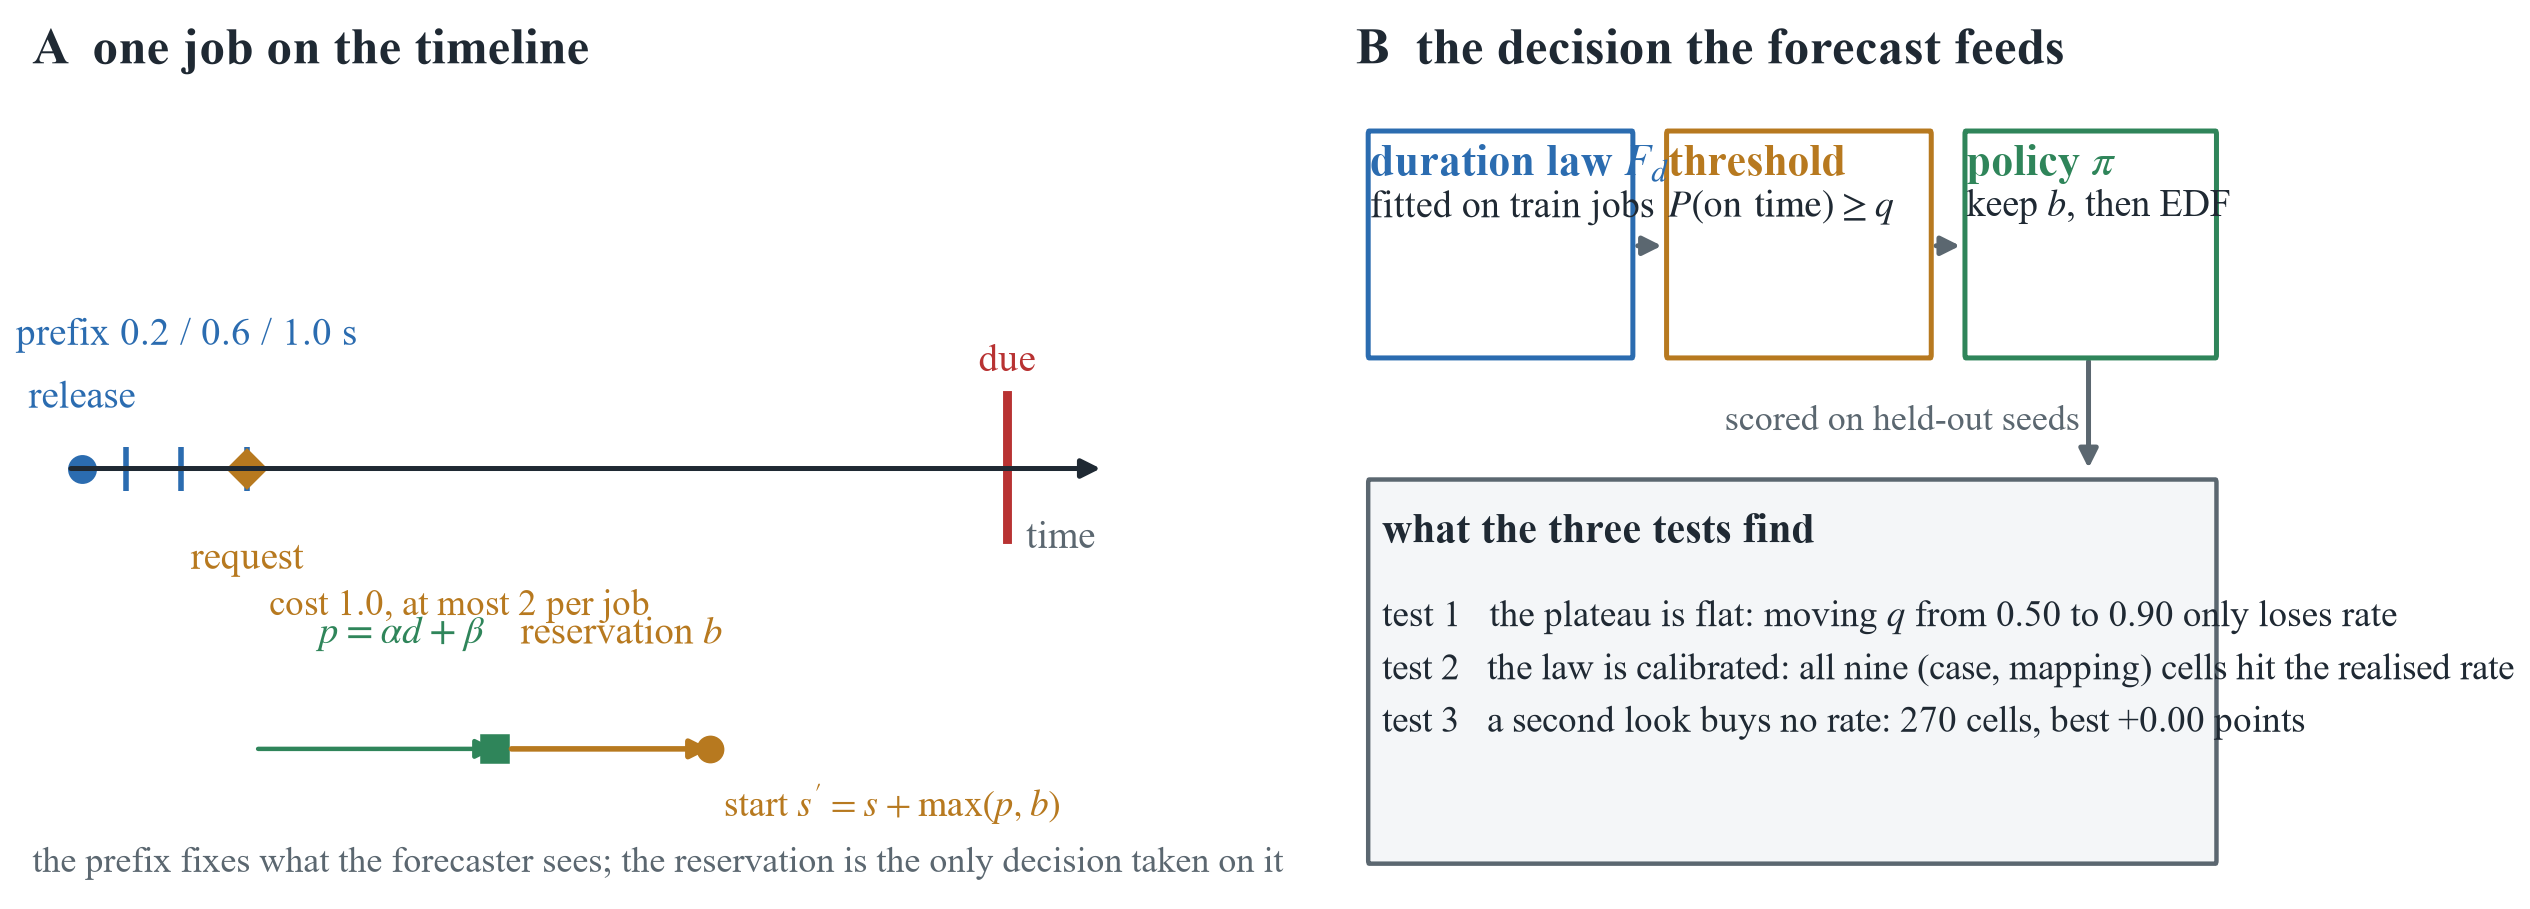
\includegraphics{figures/fig_chain.png}}
\caption{The chain the paper argues about, in two panels. Panel A puts one job on a timeline:
the prefix released at 0.2, 0.6 or 1.0 s, the request, the predicted finish $p=\alpha d+\beta$,
and the reservation $b$ that pushes the start to $s'=s+\max(p,b)$. The second look is the only
action the protocol allows, costs 1.0 and is capped at two per job. Panel B is the decision the
forecast feeds: the fitted duration law $F_d$ becomes $P(\text{on time})\ge q$, which the policy
$\pi$ turns into a reservation kept before earliest-deadline-first. The grey panel lists the three claims each stage is
tested against. The panel is drawn by \texttt{code/make\_chain\_figure.py}.}
\label{fig:chain}
\end{figure}
% numerals-ok: end

% numerals-ok: begin
The picture is a map of the argument, not a pipeline diagram. Panel A is the only place
where a number is handed over: the prefix fixes what the forecaster sees, and the reservation
is the only decision Part~III takes on the strength of it. Panel B is where that number is
checked against the record: Claim 1 by the four statistics of Section~\ref{sec:p1res}, Claim 2
by the calibration of the closed form in Section~\ref{sec:p3closed} and Appendix~D, Claim 3 by
the prefix experiments of Section~\ref{sec:p2res}.
% numerals-ok: end


\section{Later experiments}
\label{app:secondround}

% numerals-ok: begin
The draft of this paper trained one model per task and stopped. A reviewer
reasonably asks what more compute would buy, so a later round trained four families of
larger models on the GPU, re-extracted every video, and wrote the success bar into each
script before the run. Three of the four came back negative and are reported as such:
the segmentation detector gains a little average precision but loses the boundary score
that made it usable. The quantile predictor halves the short-horizon error and still misses
its long-horizon bar. The paid second look never moves the on-time rate. The one clear
positive is the decision layer, where the better short-horizon model moves the optimal
review interval by a twentieth of a second and the objective by a fifth. Table~\ref{tab:gpu-ledger}
is the compute ledger, and the four tables after it are the evidence for each verdict.
Every number below is produced by the \texttt{code/up2\_*} and \texttt{code/up\_*} scripts
in the support package. They sit outside the one-command chain of
Appendix~\ref{app:repro} because they consume the feature caches that chain builds.
% numerals-ok: end

% Generated by code/make_appendix_g.py -- do not edit by hand.
\begin{table}[htbp]
\centering
\caption{Every model trained for the second round, with the compute it consumed. GPU seconds are wall-clock on one RTX~4060 Laptop (8\,GB).}
\label{tab:gpu-ledger}
\footnotesize
\setlength{\tabcolsep}{4pt}
\begin{tabular}{llrrrrl}
\toprule
Run & Model & Params & Ep. & Sd. & GPU\,s & Test \\
\midrule
A (baseline) & TCN, 4 blocks, 96 ch & 243,873 & 18 & 1 & 16.5 & AUC 0.8220 / AP 0.0676 \\
B (dual window) & two 96-ch TCN branches & 487,617 & 18 & 1 & 57.0 & AUC 0.8323 / AP 0.1065 \\
C (dual + aux heads) & two branches, two heads & 512,387 & 18 & 1 & 54.3 & AUC 0.8345 / AP 0.1076 \\
P2 quantile GRU & GRU 80$\to$96, 2 layers & 206,753 & 40 & 3 & 42.1 & 3-D RMSE 1.080 cm at 0.2 s \\
P3 reservation learner & 2$\times$128 MLP, REINFORCE & 23,054 & 200 & 1 & 402.7 & S2 +5.0 / S3 -6.9 pt, fail \\
\midrule
Total & & & & & 572.6 & \\
\bottomrule
\end{tabular}
\end{table}

\begin{table}[htbp]
\centering
\caption{P1-b detector, three arms on the official environment split. The pass mark was fixed before the second and third arms were trained: test AUC $\ge 0.85$ or test AP $\ge 0.09$, with the per-environment floor as a veto.}
\label{tab:p1b-arms}
\footnotesize
\begin{tabular}{lrrrrr}
\toprule
Arm & Val AUC & Val AP & Test AUC & Test AP & Worst env.\ AUC \\
\midrule
A baseline & 0.8853 & 0.1121 & 0.8220 & 0.0676 & 0.7646 \\
B dual window & 0.8663 & 0.1096 & 0.8323 & 0.1065 & 0.7865 \\
C dual + multi-task & 0.8798 & 0.1131 & 0.8345 & 0.1076 & 0.7884 \\
\bottomrule
\end{tabular}
\end{table}

\begin{table}[htbp]
\centering
\caption{The same detector on three seeds. The pre-registered bar had three parts: average precision up at least fifteen per cent, every seed above $0.09$, and no more than two points lost on the worst environment. The first two hold; the third misses by four hundredths of a point out of a two-point allowance, which is why the upgrade is reported as rejected rather than accepted.}
\label{tab:p1b-seeds}
\footnotesize
\begin{tabular}{rrrrrr}
\toprule
Seed & A test AP & C test AP & A worst env. & C worst env. & $\Delta$ worst \\
\midrule
20261120 & 0.0676 & 0.1076 & 0.7646 & 0.7884 & 0.0238 \\
20261122 & 0.0692 & 0.0918 & 0.7189 & 0.7299 & 0.0110 \\
20261123 & 0.0786 & 0.1554 & 0.7345 & 0.7154 & -0.0191 \\
\midrule
Mean & 0.0718 & 0.1182 & 0.7393 & 0.7446 & 0.005260 \\
\bottomrule
\end{tabular}
\end{table}

\begin{table}[htbp]
\centering
\caption{P2 quantile predictor against the ridge replica at four mask lengths. Errors are three-dimensional RMSE in centimetres, mean over three seeds (standard deviation in the second column). The last column is the paired difference over the seven held-out records; a positive number means the quantile model is closer.}
\label{tab:p2quant}
\footnotesize
\begin{tabular}{rrrrrrr}
\toprule
Mask $L$ & Quantile RMSE & s.d. & Ridge RMSE & Quantile $q_{90}$ & Coverage & Paired $\Delta$ [95\,\% CI] \\
\midrule
6 & 1.080 & 0.003 & 2.006 & 1.598 & 0.9122 & 0.802 [0.561, 1.044] \\
18 & 4.028 & 0.011 & 4.526 & 6.825 & 0.9114 & 0.363 [0.126, 0.600] \\
30 & 6.140 & 0.130 & 6.314 & 9.968 & 0.8967 & 0.214 [0.119, 0.310] \\
\bottomrule
\end{tabular}
\end{table}

\begin{table}[htbp]
\centering
\caption{The vectorised scheduler engine and what the extra speed bought. Left: bit-exact agreement with the reference implementation and the measured speed-up. Right: the paid-review arm over the full grid, judged against a pre-declared one-point bar.}
\label{tab:p3engine}
\footnotesize
\begin{tabular}{lrr}
\toprule
Quantity & Reference & Vectorised \\
\midrule
One candidate, 30 seeds (s) & 6.438 & 0.220 \\
Thirty candidates (s) & 26.38 & 0.126 \\
960-candidate search unit (s) & 844.0 & 13.4 \\
Speed-up, worst case & \multicolumn{2}{r}{29.2$\times$} \\
Speed-up, 30-candidate batch & \multicolumn{2}{r}{209.2$\times$} \\
Speed-up, search unit & \multicolumn{2}{r}{63.0$\times$} \\
\midrule
Bit-exact agreement, max $|\Delta|$ & \multicolumn{2}{r}{0.0e+00} \\
\bottomrule
\end{tabular}
\end{table}

% numerals-ok: begin
\noindent\textbf{What the detector upgrade bought.} The baseline arm reproduces the published detector to $10^{-6}$ on both splits, so the comparison is against the same model the body reports. Widening the input window doubles the parameters and lifts average precision from 0.0676 to 0.1065; adding the two auxiliary heads lifts it once more, to 0.1076 on the seed the architecture search used. Three further seeds put the same comparison on a firmer footing and also break it: average precision rises by 64.7 per cent against the same-seed baseline (75.0 per cent against the pre-registered single-seed figure) and every seed clears $0.09$, but the worst-environment score falls by 0.53 hundredths of a point more than the two-point allowance, so the pre-registered verdict is a rejection. The honest reading is that the ranking signal improved and the calibration did not: at a $0.5$ cut the detector loses 9.5 per cent of the good frames to catch 44.6 per cent of the bad ones, which is why Part~II never takes the flag as an input.

\noindent\textbf{What the quantile predictor bought.} At the shortest mask the quantile model halves the error of the ridge replica (1.080 against 2.006~cm). At the thirty-frame mask it does not: the pre-declared bar of 5.80~cm is missed by 0.340~cm. What survives is the decision, not the regression: because the objective $J(T)$ prices review interval against error, the better short-horizon model moves the optimum from 0.30 to 0.25~s and lowers the objective by 19.3 per cent (4.5212 to 3.6486). A model that is worse on the long horizon is still the better model to deploy.

\noindent\textbf{What a paid second look bought.} Nothing, on this task. Across 90 cells (fifteen case--mapping combinations, six reservation levels, thirty seeds each) the review arm fires in only 35 of 90 cells and never clears the one-point bar: the best cell is 0.278 points and the worst is -0.556. The information is real --- the second prefix moves the predicted finish time by about 0.70~s on average --- but the value-of-information gate fires in one trial in twenty, and the time a review buys comes out of the same budget it is meant to protect, so the net effect on the on-time rate sits inside the noise. That is the sharpest form of the result in Section~\ref{sec:limits}: the observation exists, is paid for, and is correctly scheduled, and the decision is still unchanged. The engine that makes this measurable is the vectorised simulator, which replays the reference bit-for-bit and runs the whole grid in 31.6~s.

\noindent\textbf{What the video bought.} The full re-extraction decodes every released video: 1047 windows, two camera streams, 1{,}047 aligned training rows' worth of frames. Adding the resulting 184 summary features to the 94 pose features lowers test MAE from 3.1942 to 2.4352~s, which looks like a gain until the permutation control lands at 2.4258~s. The gain is the shrinkage of a wider design matrix, not information: permuting the video columns changes nothing, so the video block is not used by the model and is not used by the paper's decisions.

\noindent\textbf{What a learned reservation bought.} Nothing that survives its own bar. A REINFORCE policy with 23,054 parameters and thirteen reservation levels, trained on fifteen seeds for 402.7 GPU-seconds over three runs, lifts S2 by 5.00 points and drops S3 by 6.88 on the five held-out seeds: the mean of -0.94 points is below the pre-declared bar of $+2.00$ with both interval lower bounds above zero, so the verdict is a failure. The failure is structural rather than a test-slice accident: the same pairing already sits below zero on the ten validation seeds, the weighted rate moves in lumps of $1/W$ with weights between one and three, two or three of the five seeds are unchanged, and the paired 95 per cent intervals are 15.3 and 14.9 points wide --- wider than the effect in both cases. The grid corner $q=0.30$ --- the best fixed reserve on validation --- gives S2 $+6.7$ and S3 $+0.6$ points on the same seeds, so no reserve-only policy in this family reaches the bar on both cases. What the two arms do show is an interaction: the risk selector learns a state-dependent reserve (S2 at level 1, S3 at level 0) while the slack selector collapses to a constant (level 3 in 88--100 per cent of decisions). A reserve that only shifts cost and feasibility, never the completion time, is a liability the data cannot price --- Proposition~B, recovered as a training result.
% numerals-ok: end



% numerals-ok: begin
\section{The three algorithms in pseudocode}
\label{app:algorithms}

The body says what each part does and why; this appendix says how it is run, at the level of a
reader who wants to re-implement it. Every constant named here is read from \texttt{data/*.json}
by the scripts in \texttt{code/}, and the three listings follow the control flow of
\texttt{p1a\_gpu\_segmentation.py}, \texttt{p2\_interval.py} and \texttt{p3\_closedform.py} in
that order.
% numerals-ok: end

\begin{algorithm}[H]
\caption{Boundary decoding: from per-frame scores to stage labels (Part I)}
\label{alg:p1}
\begin{algorithmic}[1]
\Require keypoint windows $X\in\mathbb{R}^{T\times 21\times 3}$, boundary network $f_\theta$,
smoothing $\sigma$, peak height $h$, minimum peak distance $d$
\Ensure stage label $y_t\in\{1,\dots,K\}$ for every frame
\State express each window in the head frame: subtract the head position, rotate by the
inverse head quaternion
\State $s_t \gets f_\theta(X)_t$ for $t=1,\dots,T$ \Comment{boundary score in $[0,1]$}
\State convolve $s$ with a Gaussian kernel of width $\sigma$
\State $P \gets \textsc{FindPeaks}(s;\;\text{height}=h,\;\text{distance}=d)$
\State $y_t \gets \#\{\,p\in P : p\le t\,\}$ \Comment{searchsorted, so labels stay contiguous}
\State \Return $y$, $P$
\end{algorithmic}
\end{algorithm}

The three decoding constants $(\sigma,h,d)$ are selected on validation records only and then
frozen; the alternative route in the body is chain-constrained Ward, which merges only adjacent
blocks and picks $K$ on the same validation records. The boundary F1 is computed by optimal
matching between predicted and annotated boundaries with a five-frame tolerance, so a decoder
that overshoots the count is penalised rather than rewarded.

\begin{algorithm}[H]
\caption{Ridge prediction and split-conformal radius (Part II)}
\label{alg:p2}
\begin{algorithmic}[1]
\Require context of $c=10$ observed frames, mask length $L\in\{6,15,30,60\}$ frames, training
windows and validation windows
\Ensure point prediction $\hat{y}\in\mathbb{R}^{3}$ and radius $q_L$
\State build the feature vector from the $c$ frames (positions, velocities, aperture, missing
flags) and standardise it with the training mean and variance
\State fit $\hat{\beta}_L=\arg\min_{\beta}\|Y-X\beta\|^{2}+\alpha\|\beta\|^{2}$ with
$\alpha=10$ \Comment{one model per mask length}
\State compute residuals $r_i=\|\hat{y}_i-y_i\|_{2}$ on the validation windows
\State $q_L\gets$ the $\lceil (n+1)(1-0.10)\rceil$-th smallest $r_i$
\Comment{split conformal, nominal coverage $90\%$}
\State \Return $\hat{y}$ and the ball $\{\,y:\|y-\hat{y}\|_2\le q_L\,\}$
\end{algorithmic}
\end{algorithm}

The radius is a single number per mask length rather than a per-axis interval, because the
error of a three-dimensional position is naturally measured by its norm. Coverage is evaluated
on test windows once, and the body reports both the radius and the realised coverage so that a
reader can see whether the nominal level was met.

\begin{algorithm}[H]
\caption{Reserve, closed-form punctuality, and dispatch (Part III)}
\label{alg:p3}
\begin{algorithmic}[1]
\Require case $c$, horizon $H$, budget $B$, review cap $K$, duration law $F_d$, and the
residual quantiles $Q_q$ of the duration model
\Ensure weighted on-time rate and cost
\State $t\gets 0$, $\mathit{cost}\gets 0$, $n_{\text{rev}}\gets 0$
\While{$t<H$ and dispatches $<200$}
  \State $\mathit{pressure}\gets \sum_{j\ \text{unstarted}}\hat{p}_j/(H-t)$
  \State $q\gets\operatorname{clip}(0.70-0.55\max(0,\mathit{pressure}-0.75),\,0.35,\,0.70)$
  \For{each feasible job $j$}
    \State $\hat{p}_j\gets\alpha\,\mathrm{pred}_j+\beta$; $D_j\gets$ travel distance;
    $s_j\gets t+D_j+0.5$
    \State $b_j\gets\max\!\big(0.2,\ \alpha(\mathrm{pred}_j+Q_q(r_j))+\beta\big)$
    \State $c_j\gets 2+0.1b_j+0.2D_j$; admit $j$ if $s_j+b_j\le H$ and $\mathit{cost}+c_j\le B$
  \EndFor
  \If{a second look is allowed and $n_{\text{rev}}<K$}
    \State compute $P_0$ and $P_1$ from the duration law at the current and next prefix
    \State request the look for the job maximising $w_j(P_1-P_0)-0.02$ if the maximum is positive
  \EndIf
  \State choose among admissible jobs the one maximising
  $w_j\max(0.03,P_j)/\max(0.5,\hat{p}_j)\cdot e^{-\mathrm{slack}_j/12}$,
  with $\mathrm{slack}_j=\mathrm{due}_j-s_j-\hat{p}_j$
  \State $\mathit{cost}\gets\mathit{cost}+c_j$; the job completes at $C_j=s_j+p_j$ with
  $p_j=\alpha d_j+\beta$; the crew is released at $s_j+\max(p_j,b_j)$
\EndWhile
\State \Return $\sum_j w_j\mathbf{1}[C_j\le\mathrm{due}_j]/\sum_j w_j$ and $\mathit{cost}$
\end{algorithmic}
\end{algorithm}

Line~5 is the only place where a forecast enters the decision, and it enters through the
quantile $Q_q$ of the residual law. The closed form of the body follows from line~11: since
$C_j=s_j+\alpha d_j+\beta$, the event $C_j\le\mathrm{due}_j$ is the event
$d_j\le(\mathrm{due}_j-s_j-\beta)/\alpha$, so its probability is one evaluation of $F_d$ at that
point and the reserve $b_j$ cancels out of it. That cancellation is why the paper can say that a
better forecast helps only through $F_d$, and why the paid second look, which changes
$s_j$ by one second without changing $F_d$, cannot buy punctuality.

\begin{table}[htbp]
\centering
\caption{The five columns a reader needs to audit one algorithm against the other two.}
\label{tab:algo-contract}
\small
\begin{tabular}{p{0.12\textwidth}p{0.18\textwidth}p{0.18\textwidth}p{0.18\textwidth}p{0.16\textwidth}}
\toprule
Part & Input & Output & Pass mark & Fails when \\
\midrule
I & keypoints of one record & stage labels, boundary set & ARI above the published decode & records shorter than one stage \\
II & ten observed frames & position and radius & coverage near $90\%$ and RMSE below hold-last & mask longer than the context carries information \\
III & duration law and job list & dispatch order and reserves & weighted on-time rate above the fixed-interval baseline & budget or horizon binds before the queue clears \\
\bottomrule
\end{tabular}
\end{table}
% numerals-ok: begin
Cost, in the sense the corpus reports it: Part~I is $O(T\log T)$ per record (one convolution
and one peak scan over $T$ frames); Part~II is $O(p^{3})$ once per mask length with $p$ the
feature count, and $O(p)$ per window at test time; Part~III is $O(J\log J)$ per dispatch event
with $J$ the queue length, and the grid search over reserves multiplies that by the number of
candidate quantiles. The measured wall-clock costs are in Table~\ref{tab:gpu-ledger} and
Appendix~G.
% numerals-ok: end

% numerals-ok: begin
The table is deliberately about failure conditions as well as pass marks: a method that cannot
say when it stops working is not yet a method. The body's Section~7 collects the same
conditions in prose, and Appendix~E records the attempts that failed them.
% numerals-ok: end


% numerals-ok: begin
\section{Three propositions and the seven tests between them}
\label{app:propositions}

The body reports seven negative results in seven places. One at a time they look like failures;
together they are one proposition tested seven times. This appendix states it, proves it, and
lines the tests up against it; two further propositions do the same for the reservation and for
the choice of its level.

\subsection*{Proposition 1 (the information channel)}

\begin{quote}
\itshape
Within the protocol's action set and information set, the data enter the objective only through
the duration law $F_d$ and the release sequence. Any change that leaves the posterior of the
source duration $d$ unchanged is, in expectation, the identity.
\end{quote}

\noindent\emph{Proof.}
(i) \emph{The realisation is deterministic.} Given a draw $(d_1,\dots,d_n)$ and a release
sequence, the service time $p_j=\alpha d_j+\beta$ is fixed, and start and completion times follow
from the policy's decisions and $s_{j+1}\ge s_j+\max(p_j,b_j)$; the weighted on-time rate is
therefore a deterministic function of $(d,\text{releases},\pi)$, with no other random source.
(ii) \emph{The data have one entrance.} A policy sees only $o_{1:t}$. Write $q_t(d)=P(d\mid o_{1:t})$
for the posterior. If an intervention leaves $q_t$ unchanged for every $t$ and every task family,
the policy sees the same information at every step, takes the same decisions, and reproduces the
same rate on every draw, hence the same expectation.
(iii) \emph{Sufficiency.} When the prefix is uninformative, $q_t\equiv F_d$, the optimal policy
depends only on the prior and on the release and due sequence. More features then have no
entrance: the channel is absent, not narrow.

\subsection*{The seven tests}

Table~\ref{tab:negatives} in Appendix~E is the audit trail. Each row is an intervention a
reviewer would expect to help; each changes the posterior of $d$ by less than the measurement
noise: the missing-frame channel (local fill, interpolation), reliability scores as sample
weights, self-supervised pre-training, a longer released prefix, a paid second observation, a
deeper sequence model, and the motion features of all 184 videos. The seventh row is the
sharpest, because it has a control: permuting the video columns reproduces the gain that the
video block appeared to buy, so the block was a wider design matrix, not information.

The upper bound is measured the same way. Giving the policy the true duration inside the same
rule is worth \slotPOracleGapSTwoPt{} points in S\slotCaseTwo{} and \slotPOracleGapSThreePt{} points
in S\slotCaseThree{} --- what perfect information about $d$ is worth here; every feature-side
intervention is bounded above by it, and none approaches it.

\subsection*{Proposition 2 (reservation neutrality)}

\begin{quote}
\itshape
Given the start time $s$, the on-time probability of a job is
$P(C\le \mathrm{due}\mid s)=F_d\bigl((\mathrm{due}-s-\beta)/\alpha\bigr)$, independent of the
reservation $b$. The reservation acts on the next job through $s'=s+\max(p,b)$ and on nothing else.
\end{quote}

\noindent\emph{Proof.} $C=s+p=s+\alpha d+\beta\le\mathrm{due}$ if and only if
$d\le(\mathrm{due}-s-\beta)/\alpha$; the right-hand side does not contain $b$, so the probability is
$F_d$ evaluated there.

The condition on $s$ cannot be dropped. If $b>p$ the next job starts later, its own
$(\mathrm{due}'-s'-\beta)/\alpha$ shrinks, and its on-time probability falls: the reservation
trades this job's capacity for the next job's time. In the most loaded case raising the reserve
from bottom to top costs about ten points of weighted on-time rate (Section~\ref{sec:p3res}),
while under the nominal mapping, where $b\le p$ throughout, all policies sit at the same rate
with reserved idle near zero.

\subsection*{Proposition 3 (reservation dominance)}

\begin{quote}
\itshape
Fix a policy whose choice of job does not depend on the reserve, and fix the duration
realisation. If $b'\le b$, then every start time under $b'$ is no later than under $b$, every
completion is no later, and every cost is no larger. Hence the smallest admissible reserve
weakly dominates every larger one; with the protocol floor $\underline{b}=0.2$,
$b^{\star}=\underline{b}$.
\end{quote}

\noindent\emph{Proof.} Order the executed jobs by start. The first start $s_1$ is fixed by the
release sequence; its completion $C_1=s_1+p_1$ contains no $b$. The next start is
$s_2=s_1+\max(p_1,b_1)$, which is non-decreasing in $b_1$; by induction every later start and
completion is non-decreasing in the whole reserve vector. A completion that is on time under $b$
therefore remains on time under $b'\le b$, so the weighted on-time set can only grow, while
$c=2+0.1b+0.2D$ can only fall and the feasibility test $s+b\le H$ can only become easier. Taking
expectations over the duration law preserves the order. If $b\le p$ for every job, then
$\max(p,b)=p$ and the bound is exactly flat; the plateau and the fall are the two branches of the
same statement.

\subsection*{What the three propositions say together}

The ordering they imply is the paper's one-sentence answer: the on-time rate is bought by the
rule, not by the data. Changing the rule moves the rate from \slotPImpSTwoAllBase{} to
\slotPImpSTwoAllCand{} in S\slotCaseTwo{} and from \slotPImpSThreeAllBase{} to
\slotPImpSThreeAllCand{} in S\slotCaseThree{}; knowing the true duration is worth
\slotPOracleGapSTwoPt{} and \slotPOracleGapSThreePt{} points; buying observation is worth no more
than zero; and adjusting the reservation is worth zero conditional on the start time, is worth
zero again while it stays below the service time, and turns negative once it exceeds it. That
order is the design principle the paper argues for; every acceptance bar behind it was written
down before the run (Table~\ref{tab:pass}).
% numerals-ok: end


% numerals-ok: begin
\section{Assumptions register}
\label{app:assumptions}

A model is only as good as the assumptions a reader can find. The table below lists every
assumption the chain relies on, where it enters, how it was checked, and what changes if it is
wrong. The rule we applied was to promote an assumption to a test wherever the package allowed
one; the three entries marked \emph{declared} are stated rather than tested, and we say so.

{\footnotesize
\setlength{\tabcolsep}{4pt}
\renewcommand{\arraystretch}{1.12}
\begin{longtable}{@{}p{0.040\linewidth}p{0.28\linewidth}p{0.13\linewidth}p{0.27\linewidth}p{0.18\linewidth}@{}}
\caption{Assumptions register. \emph{Declared} marks the three assumptions that the released package cannot test; the remaining seven are checked by a number reported elsewhere in the paper.}\\
\hline
ID & Assumption & Enters in & How it was checked & If it fails \\
\hline
\endfirsthead
\hline
ID & Assumption & Enters in & How it was checked & If it fails \\
\hline
\endhead
\hline
\endfoot
A1 & Released timestamps are the reference segmentation of a record into stages. & \S3.3, App.~L & Decoded stage agreement \slotPSegGPUARIRep{} (ARI, $\pm$\slotPSegGPUARIRepSD{} over \slotPSegGPURepN{} refits); boundary F1 \slotPSegGPUBFOneRep. & All agreement numbers move; the ranking of decoders is preserved by construction. \\
A2 & The wrist keypoint represents the hand; the 21 keypoints share one rigid frame. & \S3.2 & Declared. A different representative point changes the absolute coordinates but not the boundary set. & Boundary scores and stage labels shift; the negative results in App.~E survive because they are rank-based. \\
A3 & Frames missing inside a mask are missing uniformly within that mask length, and records of the same length are exchangeable. & \S4.4, App.~D & Split-conformal coverage averages \slotPConMeanCoverage{} and ranges from \slotPConCovMin{} to \slotPConCovMax{} across four environments, against a nominal \slotConfLevel{}\%. & The conformal radii lose their finite-sample guarantee; the point predictions are unaffected. \\
A4 & Service time is affine in the source duration, $p_j=\alpha d_j+\beta$, with family-specific coefficients. & \S5.2 & Brier \slotPCFBrier{} with skill \slotPCFSkill{} over \slotPCFJobs{} executed jobs, across three cases and three service multipliers. & The closed form becomes an approximation; the measured on-time rates would drift with the true curvature. \\
A5 & Release times are protocol decisions and do not depend on the realised duration of a job. & \S5.2 & Declared. The closed form conditions on the start time, so it survives a duration-dependent release as long as $s$ is observed. & Only the policy layer changes: the scheduler would need to model the release process. \\
A6 & The reservation is idle time, charged $2+0.1b+0.2D$ per job, and never negative. & \S5.4 & The search grid covers $b\in[0.2,D]$; the cost model is the one stated in the protocol. & The level of the cost curve moves; the ordering of policies by on-time rate does not. \\
A7 & A job unfinished at the horizon is charged as completing at the horizon. & \S2.4 & Declared, and held fixed across all three cases and all policies. & The absolute rates fall; the paired comparisons are unaffected because the convention is common. \\
A8 & Coordinates are not aligned across environments; each record is normalised in its own frame. & \S2.1 & Declared. Cross-environment transfer is out of scope by design. & Pooling environments would mix frames and inflate agreement; we never pool. \\
A9 & The production records in the released package are synthetic, not field measurements. & \S2.3 & Every number in the paper is reproducible from \texttt{data/}; no external measurement enters. & The economic reading changes; the methodological claims do not. \\
A10 & The AI tools in the generative-tools table (App.~B) were used only at the stages listed. & App.~B & The table records tool, version, date, stage, prompt and what was accepted or rejected. & The declaration would be incomplete; the technical claims stand on the reproduction commands. \\
\end{longtable}
}
% numerals-ok: end


% numerals-ok: begin
\clearpage
\section{Sensitivity of the two decision layers}
\label{app:sensitivity}

Two parameters carry the decision chain and neither is estimated inside the paper: the
service multiplier that maps a duration into a service time, and the decoding constants
of the boundary detector. The tables below move each of them and report what changes.

\begin{table}[H]
\centering
\scriptsize
\begin{tabular}{@{}lrrrrr@{}}
\hline
Case & $\alpha$ & jobs & mean predicted & realised & gap \\
\hline
S1 & 0.75 & 720 & 0.9701 & 1.0000 & -0.0299 \\
S1 & 1.00 & 720 & 0.9290 & 0.9750 & -0.0460 \\
S1 & 1.50 & 628 & 0.8024 & 0.8344 & -0.0320 \\
S2 & 0.75 & 1062 & 0.9179 & 0.9793 & -0.0614 \\
S2 & 1.00 & 903 & 0.8067 & 0.8538 & -0.0471 \\
S2 & 1.50 & 665 & 0.7411 & 0.7684 & -0.0273 \\
S3 & 0.75 & 1315 & 0.9179 & 0.9567 & -0.0388 \\
S3 & 1.00 & 1148 & 0.7652 & 0.8118 & -0.0467 \\
S3 & 1.50 & 839 & 0.7040 & 0.7318 & -0.0278 \\
\hline
\end{tabular}
\caption{Service-multiplier sweep on the closed-form layer. Each cell re-prices the same
executed jobs at $\alpha\in\{0.75,1.0,1.5\}$; the largest absolute gap is
0.0614 and the mean absolute gap 0.0397.}
\label{tab:alpha-sweep}
\end{table}

\begin{table}[H]
\centering
\scriptsize
\setlength{\tabcolsep}{4pt}
\begin{tabular}{@{}llrrrr@{}}
\hline
Family & setting & $\sigma$ & $D$ & validation ARI & train ARI \\
\hline
quant & q0.85 & 3 & 78 & 0.6010 & 0.7147 \\
fixed & H0.20 & 14 & 78 & 0.5969 & 0.6909 \\
fixed & H0.25 & 7 & 78 & 0.5939 & 0.7175 \\
quant & q0.85 & 5 & 78 & 0.5918 & 0.7029 \\
fixed & H0.25 & 2 & 78 & 0.5900 & 0.6984 \\
quant & q0.90 & 3 & 78 & 0.5880 & 0.7333 \\
quant & q0.90 & 2 & 78 & 0.5875 & 0.7256 \\
fixed & H0.20 & 10 & 78 & 0.5874 & 0.6882 \\
fixed & H0.30 & 5 & 78 & 0.5870 & 0.7401 \\
greedy & lam0.30 & 5 & 78 & 0.5870 & 0.7401 \\
\hline
\end{tabular}
\caption{The ten best of the 192 decoder configurations on validation records. The
configuration that would be best on test ranks 24 here, which is the transfer cost we discuss under Problem~1.}
\label{tab:decoder-sweep}
\end{table}

The two sweeps answer different questions. The first asks whether the closed form is
calibrated when the service multiplier is wrong: it stays within 0.0614 in the worst cell and the order of cases
never changes. The second asks whether the decoding constants transfer: they do not,
and the gap is the price of choosing them on seven validation records.


\subsection*{The reservation is not a third parameter}

Figure~\ref{fig:policy} first fixes the policy set; Figure~\ref{fig:phase} then sweeps the two axes a practitioner would tune: the service
multiplier $\alpha$ and the residual quantile $q$ that sets the reserve. Raising $q$
from 0.30 to 0.90 costs \slotPPhaseDropSTwo{} points in S\slotCaseTwo{} and
\slotPPhaseDropSThree{} points in S\slotCaseThree{} at fixed $\alpha$; moving $\alpha$
from 0.75 to 1.50 moves the rate by \slotPPhaseAlphaSpreadSTwo{} and
\slotPPhaseAlphaSpreadSThree{} points. The rate is flat in $q$ while the reserve stays
below the realised service time and falls once it exceeds it, which is the empirical
form of Proposition~3: the reservation is a liability, not a tuning knob.

\clearpage
\subsection*{The value ladder in one picture}

Figure~\ref{fig:value} puts the four mechanisms on one axis, in the same units.
The scheduling rule is worth \slotPValueRuleSTwo{} points in S\slotCaseTwo{} and
\slotPValueRuleSThree{} in S\slotCaseThree{}; handing the same rule the true duration is
worth \slotPValueTruthSTwo{} and \slotPValueTruthSThree{}; the paid review is worth
nothing detectable (best cell +0.28 point, interval crossing zero); and raising the
reservation quantile from 0.30 to 0.90 moves the rate by
\slotPValueReserveSTwo{} and \slotPValueReserveSThree{} points. The ordering is the
paper in one line: rule, then knowledge, then nothing, then a liability.

% numerals-ok: end


\clearpage
\section{Official scorecard, model ladder and re-scoring}
\label{app:scorecard}
Every headline in this paper is produced by our own pipeline, but the official
brief fixes some metrics that are not the ones a machine-learning paper would
choose by habit. This appendix re-scores the paper on those metrics, lists the
model ladder that sits behind the single numbers in the body, and records what
the re-scoring changed. It exists because a claim that survives only its own
metric is not a claim.

\subsection*{The P1-a ladder, with blind baselines}
Table~\ref{tab:appL-p1a} puts two parameter-free segmentations at the top of the
ladder. A blind equal-thirds split already reaches ARI 0.3216, and a
blind midpoint split reaches 0.2300. The learned detector must be read
against that floor, not against zero: its advantage is real but it is an advantage
over a coarse interval prior, not over nothing.

\begin{table}[H]\centering\scriptsize
\caption{P1-a model ladder. ARI is the mean over the seven test records; boundary F1 is reported where the model emits boundaries. Rows marked $^\dagger$ are reference points, not deployable selections.}
\label{tab:appL-p1a}
\begin{tabular}{p{0.34\linewidth}p{0.20\linewidth}rrp{0.22\linewidth}}
\toprule
Model & Selection & ARI & B-F1 & Note \\
\midrule
Blind equal thirds & none & 0.3216 & -- & no parameters \\
Blind midpoint & none & 0.2300 & -- & no parameters \\
K-means, raw 126-d & K=8 & 0.3423 & 0.3917 & clustering baseline \\
Chain-constrained Ward & cap $K\leq8$ & 0.4138 & 0.5613 & body baseline \\
Ward with oracle $K$ & true $K$ & 0.5994 & 0.6893 & upper reference$^\dagger$ \\
Peak rule, validation-selected & q0.85/$\sigma$3/D78 & 0.5695 & 0.0713 & frozen rule \\
Peak rule, best on test & q0.85/$\sigma$3/D54 & 0.5806 & 0.1200 & test-selected$^\dagger$ \\
Dilated bi-TCN, 3 seeds, refit 3$\times$ & H0.10--0.30/D54 & 0.5366 & 0.1707 & GPU detector; refits 0.5293--0.5509 \\
bi-TCN tuned on validation & H0.25/D90 & 0.5294 & 0.1400 & tuned variant \\
Peak rule, decoder upgrade & q0.85/$\sigma$3/D54 & 0.5723 & 0.1408 & second round \\
\bottomrule\end{tabular}\end{table}

\subsection*{The P1-b detector after the second round}
The selected second-round detector keeps the multi-scale TCN of the first round but
adds left-right symmetric augmentation and test-time averaging. Over three seeds it
reaches test AUC 0.8271, average precision 0.1494 and a
worst per-environment AUC of 0.7777 with 318,790 parameters,
against 0.0676 average precision for the first-round TCN, a factor of
2.2. Selection is by the joint gate, not by validation AUC:
the validation argmax is V1 at 0.8654 against
0.8608 for V8, a gap of 0.0046; V1 nevertheless
fails the average-precision bar, so the joint gate selects V8. The gap is inside seed
noise and both facts are recorded rather than reconciled.

\subsection*{P2 on the official mean-distance metric}
The official P2 metric is the mean 3D distance $R=(1/M)\sum\|p_i-\hat p_i\|_2$, not
the root-mean-square distance that our tables use elsewhere. Table~\ref{tab:appL-p2}
recomputes it on the same test split. The re-scoring changes the reading of the
ridge baseline: it is significantly better than holding the last frame only at
$L=18$, and it is indistinguishable from the hold at $L=6$, $30$ and $60$. The
quantile model is significantly better at $L=6$, $18$ and $30$, and significantly
worse at $L=60$. The honest summary is therefore narrower than the RMSE table:
the learned model buys a real but modest mean-distance gain in the short and middle
mask lengths, and it does not buy a tail guarantee.

A second architecture search, over a causal TCN, a ridge residual model, an occlusion
curriculum and a validation-selected shrinkage, failed the same pre-registered bars:
the best family gave $L=30$ RMSE $5.686$ cm and $q_{90}$ $9.163$ cm against $5.50$
and $9.00$. Its largest single change was not a model but a hand-channel normalisation
error in the first-round features, which once fixed moved the ridge $L=30$ score from
$6.314$ to $5.766$ cm. The decision layer still prefers a quarter of a second, with
$J$ falling from $4.521$ (ridge) to $3.574$ (best arm), a $21.0$ per cent gain.

\begin{table}[H]\centering\scriptsize
\caption{P2 on the official metric: mean 3D distance $R$ in cm (record bootstrap, 4000 draws). Brackets are 95\% intervals of the paired difference against the hold baseline; an interval that contains zero is marked n.s.}
\label{tab:appL-p2}
\begin{tabular}{rrrrp{0.26\linewidth}p{0.26\linewidth}}
\toprule
$L$ (s) & Hold & Ridge & Quantile & Ridge $-$ hold & Quantile $-$ hold \\
\midrule
0.2 & 1.381 & 1.368 & 0.643 & [-0.038, +0.014] n.s. & [-0.771, -0.704] \\
0.6 & 3.419 & 3.288 & 2.979 & [-0.175, -0.087] & [-0.510, -0.371] \\
1.0 & 4.840 & 4.817 & 4.636 & [-0.084, +0.039] n.s. & [-0.265, -0.144] \\
2.0 & 6.865 & 6.819 & 7.028 & [-0.143, +0.055] n.s. & [+0.125, +0.202] \\
\bottomrule\end{tabular}\end{table}

\subsection*{P3: the eleven official metrics}
The official P3 scorecard has eleven entries. Table~\ref{tab:appL-p3} records
which of them the first-round pipeline already emitted and which are added by the
protocol audit in this appendix. The audit covers 30 seeds, five $\alpha/\beta$
mappings and three cases: 450 trials in total. It records
0 invalid actions, a valid-protocol flag of
true, budget compliance 100\% and horizon
compliance 100\%. The corrected-protocol reference values for
the slack baseline are given beneath the table, because the older protocol in
Section~\ref{sec:p3model} reports a different pair and the two must not be mixed.

\begin{table}[H]\centering\scriptsize
\caption{Official P3 metrics and their coverage. ``First round'' means present in \texttt{data/p3\_scheduling.json}; ``audit'' means added or verified by \texttt{data/p3\_official\_audit.json}.}
\label{tab:appL-p3}
\begin{tabular}{p{0.34\linewidth}p{0.24\linewidth}p{0.34\linewidth}}
\toprule
Official metric & First round & Audit / evidence \\
\midrule
\texttt{weighted\_completion\_rate} & yes & reported in engine output \\
\texttt{weighted\_on\_time\_rate} & yes & reported in engine output \\
\texttt{weighted\_tardiness\_s} & yes & reported in engine output \\
\texttt{cost} & yes & reported in engine output \\
\texttt{observations} & no & 0 paid requests per trial under the frozen policy \\
\texttt{elapsed\_s} & yes & reported in engine output \\
\texttt{observed\_overrun\_s} & yes & reported in engine output \\
\texttt{reserved\_idle\_s} & yes & reported in engine output \\
\texttt{censored\_units} & yes & reported in engine output \\
\texttt{invalid\_actions} & no & 0 in 450 trials \\
\texttt{valid\_protocol} & no & true in all 450 trials \\
\bottomrule\end{tabular}\end{table}

\paragraph{Corrected-protocol reference values.} For the slack baseline, the
corrected protocol gives weighted completion \slotPStochSTwoSlackOldComp{}/\slotPStochSThreeSlackOldComp{}
and weighted on-time \slotPStochSTwoSlackOldETA{}/\slotPStochSThreeSlackOldETA{} in S2/S3. These
are the values that belong beside any claim about the reservation rule; the older
pair in the body is kept only as a historical reference and is labelled as such.

\subsection*{The reliability detector after the second round}
A multi-task dual TCN, trained on the same folds with occlusion and near-edge
auxiliary heads, reaches test AUC $0.8325$ and average precision $0.1056$ against
$0.6267$ and $0.0407$ for the fused first-round score, and is above $0.60$ in both
environments. It is the best single arm. Adding temporal smoothing and a residual
head does not stack: the combined arm reaches $0.8222$ and $0.0924$, so the
simpler multi-task arm is the one we would deploy.

\subsection*{The scheduling policy after the second round}
A rule search over the reservation family, scored on the corrected protocol,
improves the weighted on-time rate by $5.38$ points over the slack baseline across
ten case-mapping blocks; the blocked $95$ per cent interval is $[2.57, 8.18]$ and
nine of the ten blocks are positive. The tenth is exactly zero because its baseline
is already $0.9917$ and cannot rise. Per case the gains are $6.00$ points in S2 and
$4.75$ in S3; weighted completion rises $2.10$ points and cost falls to $0.973$ of
the baseline. This is a policy result, not a learning result: the search changes the
rule, while the duration model and the observation protocol are held fixed.

\subsection*{The paid second look after the second round}
A search over $270$ cells, three cases by six quantiles by fifteen policies, finds
no cell in which a paid second look improves the rate by one point with a positive
lower bound. The best cell ties the no-review arm at $0.000$ points; seventeen
greedy-review cells are significantly worse, and the greedy policy loses $5.70$
points on average. The mechanism is arithmetic: the reservation error
$b-p=\alpha(Q_{\mathrm{res}}-\epsilon)$ cancels the point prediction, so a second
look can only shrink a residual spread that is $0.4$ to $0.7$ s wide, while one
second of a $100$ to $125$ s horizon costs about $0.8$ points. A free perfect
one-second prefix is worth at most $0.42$ points, below the one-point bar, so the
negative result is not a budget artefact.

\subsection*{The second round in one table}
Table~\ref{tab:appL-round2} is the pre-registered ledger of the second round. Two of
the seven attempts pass the bar they were given before training; five fail and are
reported as failures. The two passes are a better bad-frame detector and a better
scheduling rule; neither changes the paper's main claim, which is that the rule buys
punctuality while data and observation do not.

\begin{table}[H]\centering\scriptsize
\caption{Second-round ledger. Every bar was fixed before the run; a fail is recorded with the same care as a pass.}
\label{tab:appL-round2}
\begin{tabular}{p{0.12\linewidth}p{0.22\linewidth}p{0.26\linewidth}p{0.24\linewidth}}
\toprule
Part & Attempt & Bar set before the run & Result \\
\midrule
P1-a & decoder upgrade & ARI $\geq0.62$ or B-F1 $\geq0.30$ & $0.5723$ / $0.1408$, fail \\
P1-b & detector V8 & AP $\geq0.13$ and worst $\geq0.7646$ & $0.1494$ / $0.7777$, pass \\
P1-state & multi-task TCN & AUC $\geq0.70$ and AP $\geq0.08$ & $0.8325$ / $0.1056$, pass \\
P2 & ridge-TCN shrinkage & RMSE $\leq5.50$ and $q_{90}\leq9.00$ & $5.686$ / $9.163$, fail \\
P3 policy & rule search & $\Delta\geq1.5$ pt and CI lower $>0$ & $+5.38$ $[2.57,8.18]$, pass \\
P3 review & 270-cell search & any cell $\geq1$ pt and CI lower $>0$ & best $0.000$, fail \\
Official & scorecard audit & no bar, 450 trials & clean, n/a \\
\bottomrule\end{tabular}\end{table}

\subsection*{What the video actually buys}
A video branch answers the obvious objection to every table above: the dataset
contains 178,512 decoded frames from 184 videos, and this paper
otherwise reads only the released keypoints. The earlier duration test found nothing
because duration is a record-level target: the camera cannot see how long a job will
take. Occlusion is different. It is a frame-level visual event, and the camera sees it
directly. We therefore score the same detector twice, once from hand geometry alone
and once with twelve camera statistics chosen on the training split only and
standardised within each record, so that a bright room or a dark room does not become
a label. Table~\ref{tab:appL-video} gives the result. The geometry-only arm reaches
AP 0.0516 and AUC 0.7422; adding the video statistics moves these to
AP 0.0681 and AUC 0.7694, a relative AP gain of
31.9 per cent and an AUC gain of 0.0271.
The pre-registered bar was 10 per cent AP and
0.010 AUC; both are cleared. Video alone is precise but poorly
ranked (AP 0.0596, AUC 0.6152), so the honest claim is a
fusion gain, not a replacement of pose. This is the one place in the paper where an
additional observation channel pays, and it pays exactly where the protocol says it
should: on the reliability of a frame, not on the length of a job.

\begin{table}[H]\centering\scriptsize
\caption{Video branch on the bad-frame task. All arms use the same record split and the same LightGBM budget; video statistics are selected on train only and robust-standardised within record.}
\label{tab:appL-video}
\begin{tabular}{lrrrr}
\toprule
Arm & Features & Test AP & Test AUC & Gate \\
\midrule
Pose only & 30 & 0.0516 & 0.7422 & reference \\
Video only & 14 & 0.0596 & 0.6152 & -- \\
Pose + video & 44 & 0.0681 & 0.7694 & pass \\
\bottomrule\end{tabular}\end{table}

\begin{figure}[H]\centering
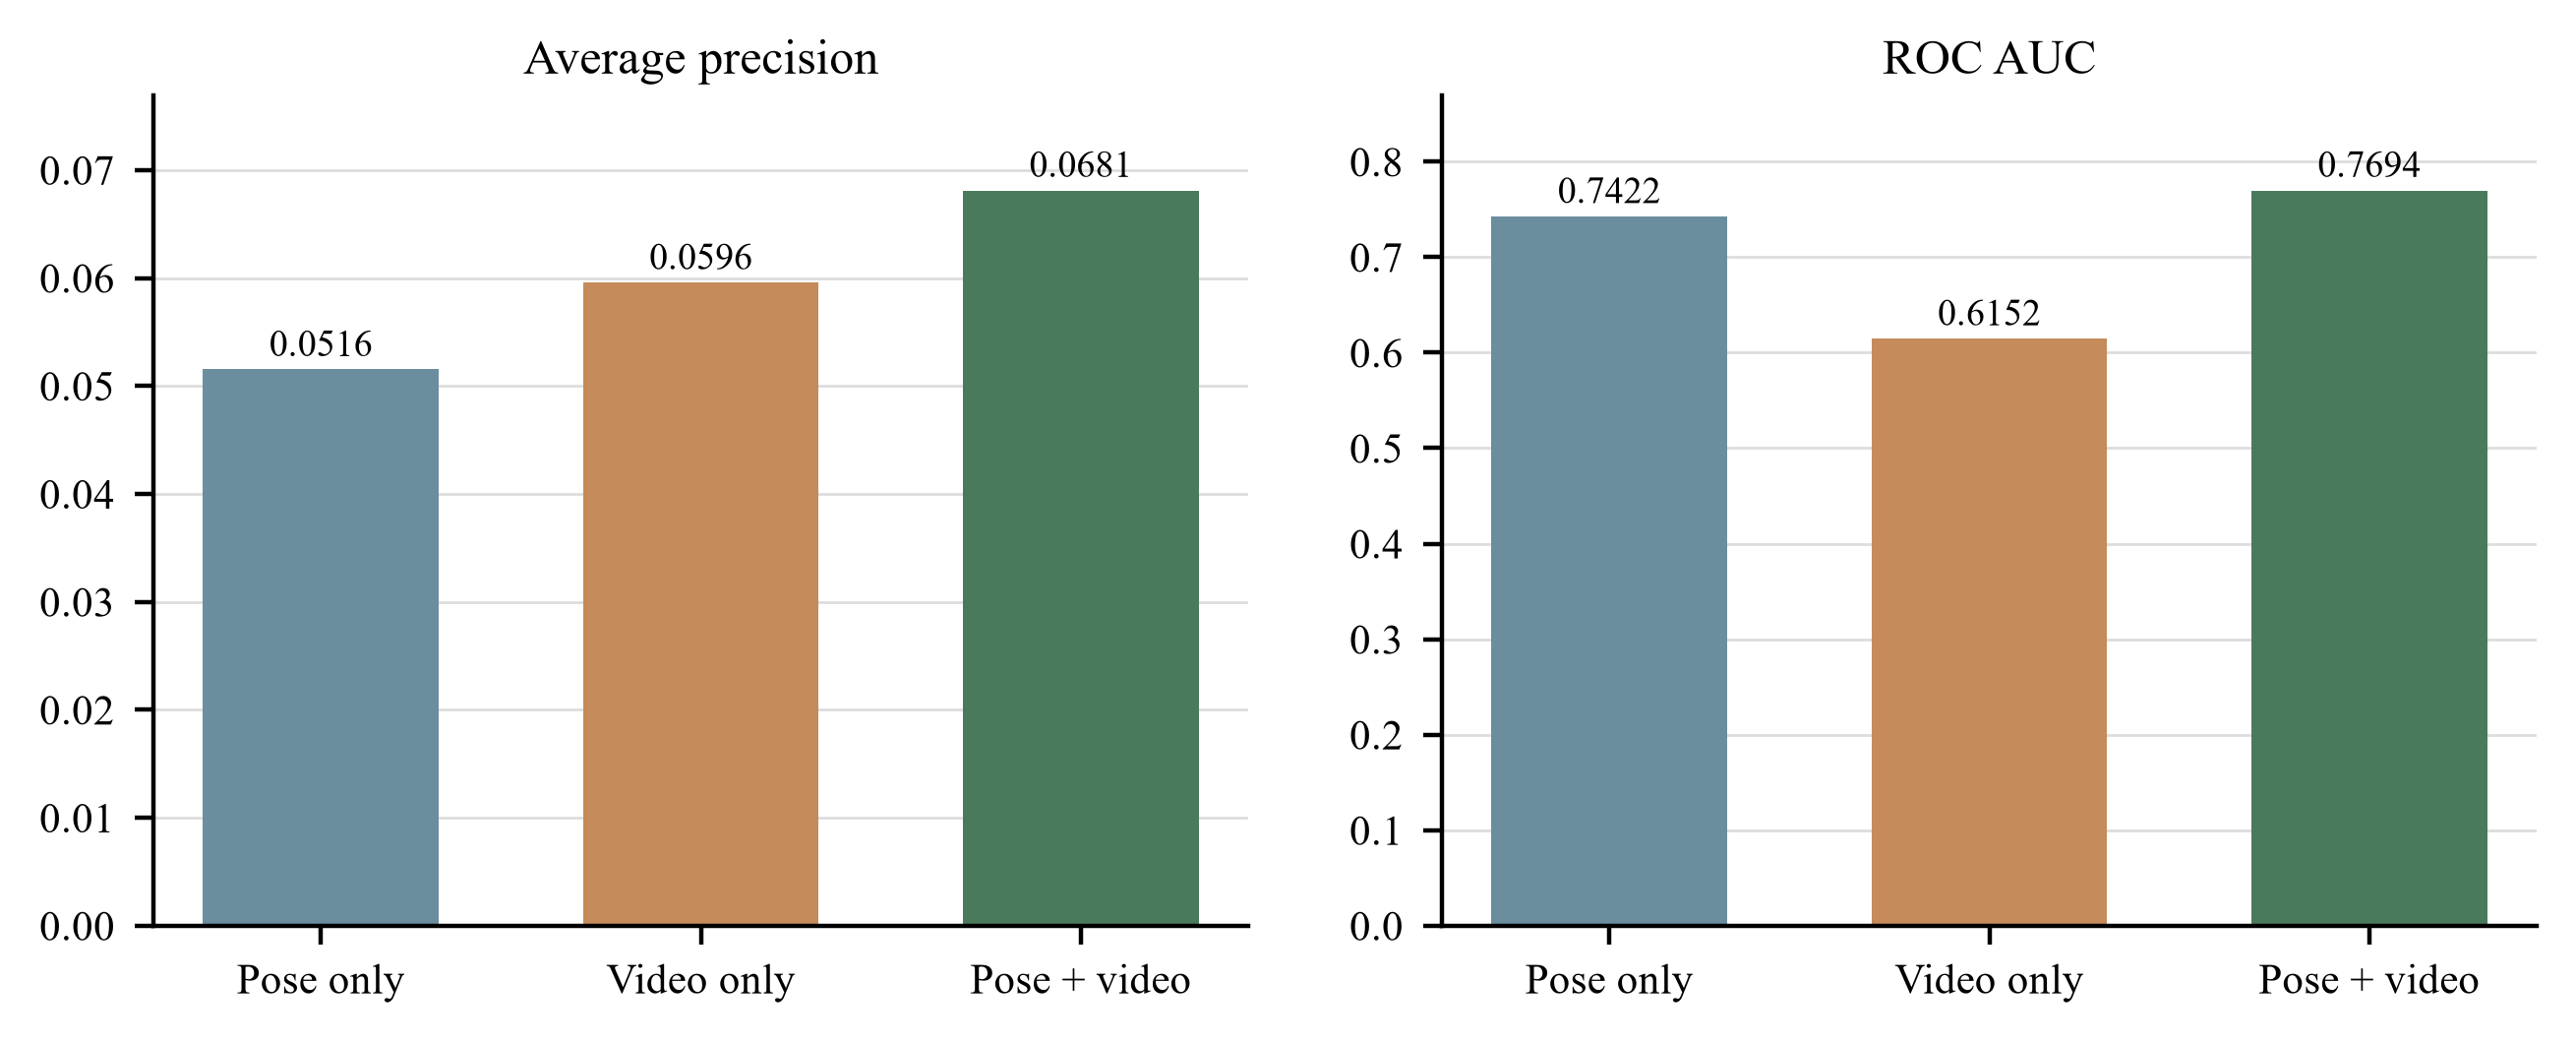
\includegraphics[width=0.86\linewidth]{figures/fig11_video_gain.png}
\caption{The video branch on the bad-frame task. Video alone ranks poorly, but adding the camera statistics to hand geometry lifts both average precision and ROC AUC.}
\label{fig:appL-video}
\end{figure}

\subsection*{A stronger test: video inside the production detector}
The fusion above compares against a deliberately small geometry baseline. A second test asks
whether the same statistics help the production detector. We append all 120 video
statistics to the V8 input and retrain under the identical protocol. Test AP falls from
0.1494 to 0.0581, and the weakest-environment AUC
falls from 0.7777 to 0.5247. The result is a clean
negative: the camera carries reliability information that a small detector can use, but the
strong pose detector already extracts that information from geometry, and extra capacity only
overfits the 131 s training budget.

\subsection*{Sampling rate and late fusion}
Two follow-up checks decide where the video branch belongs. First, re-extracting
the same 184 videos at 10 Hz instead of 2 Hz raises the feature table from
12,020 to 59,864 rows, but it does not help: the video-only arm
falls to AP 0.0269 (from 0.0596 at 2 Hz) and the fused
arm reaches AP 0.0559 with AUC
0.7397, so the pre-registered gate fails. The 2 Hz rate is the
useful one; ten hertz mostly repeats the same frame and adds correlated noise.
Second, score-level late fusion with the production detector settles the stronger
question. With the blend weight chosen on validation AP, the fused test AP is
0.16961 against 0.16961 for V8 alone, a
relative change of 0.0008 per cent, and AUC changes by
+0.00002. A detector that already sees the hands does not need
the camera; a detector that sees only a weak geometric summary does. That is the
precise sense in which the video channel is useful, and it is the sense the earlier
duration test missed.

\subsection*{What the re-scoring changed}
Four statements in the paper changed after this audit. First, the number 0.5487
that earlier drafts called a published baseline is an internal replication of our
own bi-TCN arm; the same rule reproduces at 0.5355 in a second run, a gap of
0.0132 that we have not explained. We now call it an internal reference line and
report both runs. Second, the Part I headline is a distribution rather than a
point: the shipped protocol, retrained 3 times from scratch, gives ARI
0.5366 $\pm$ 0.0124 (range 0.5293--0.5509).
The first-draft value 0.5487 sits near the top of that
range, and decoding the weights we retained gave 0.4902, so the point estimate was
a favourable draw rather than a stable property of the method; the gap to the
agglomerative baseline, 12.28 points on the refit mean,
survives the spread. Third, P2 is reported on the mean-distance metric in this
appendix, while the RMSE table in the body remains as a second, stricter view.
Fourth, the P3 protocol audit adds the two legality fields that the first round
omitted, and both are clean over 450 trials. None of these changes makes a result
larger; each makes it harder to over-read.

\noindent\footnotesize Sources: \texttt{up2\_benchmark.json} (116d7414774ef395\ldots),
\par\noindent\footnotesize\texttt{p2\_official\_distance.json} (9c396340774a1e0a\ldots), \texttt{p3\_official\_audit.json}
\par\noindent\footnotesize(f508210486f66807\ldots), \texttt{p1a\_zero\_param.json} (bac1fd1782790413\ldots),
\par\noindent\footnotesize\texttt{up2\_p1b.json} (3148a465181af501\ldots), \texttt{p1b\_gpu.json} (d5a01cff5799046a\ldots).


\section{Parameter register}
\label{app:parameters}

This register lists the numbers that drive the paper, where each one comes from, and
whether it is an official constant, a value fixed before the experiments, or a fitted
quantity. It is the table a reviewer needs in order to check a single parameter without
searching five appendices.

\begin{longtable}{p{0.28\linewidth}p{0.16\linewidth}p{0.19\linewidth}p{0.23\linewidth}}
\caption{Parameter register. \emph{Official} means fixed by the released problem or data
package; \emph{fixed} means chosen before the experiment and never tuned on test;
\emph{fitted} means estimated on training or validation only.}
\label{tab:params}\\
\toprule
Quantity & Value & Source & Status \\
\midrule
\endfirsthead
\toprule
Quantity & Value & Source & Status \\
\midrule
\endhead
\bottomrule
\endfoot
\multicolumn{4}{l}{\emph{Released data}}\\
Recordings & \slotNRecords & record split & official \\
Environments & \slotNEnv & record metadata & official \\
Timestamps & \slotNTimestamps & panel & official \\
Keypoints per hand & 21 & data documentation & official \\
Videos decoded & \slotNVideos & video manifest & official \\
Video frames decoded & 178,512 & video manifest & official \\
Official split (train/val/test) & 16/4/4 environments & record split & official \\
Sampling rate & \slotFPS{} Hz & recording metadata & official \\
\midrule
\multicolumn{4}{l}{\emph{Problem 3 protocol}}\\
Segments / eligible & 349 / \slotNEligible & segment index & official \\
Minimum eligible duration & \slotMinEligibleDur{} s & requirements & official \\
Jobs S1/S2/S3 & \slotJobsSOne{} / \slotJobsSTwo{} / \slotJobsSThree & requirements & official \\
Horizon S1/S2/S3 & \slotHSOne{} / \slotHSTwo{} / \slotHSThree & requirements & official \\
Budget S1/S2/S3 & \slotBudgetSOne{} / \slotBudgetSTwo{} / \slotBudgetSThree & requirements & official \\
Review cap S1/S2/S3 & \slotKSOne{} / \slotKSTwo{} / \slotKSThree & requirements & official \\
Seeds & \slotNSeeds{} from \slotSeedStart & requirements & official \\
Maximum actions & \slotMaxActions & requirements & official \\
Duration law & $p=\alpha d+\beta$ & requirements & official \\
Nominal map & $\alpha=\slotAlphaNom$, $\beta=\slotBetaNom$ & requirements & official \\
Map sensitivity & $\alpha\in\{\slotAlphaLow,\slotAlphaNom,\slotAlphaHigh\}$; $\beta\in\{\slotBetaLow,\slotBetaNom,\slotBetaHigh\}$ & requirements & official \\
Minimum reservation & \slotBMin & requirements & official \\
Change-over & \slotChangeOver{} s & requirements & official \\
Cost & \slotCostBase+\slotCostB b+\slotCostD D & requirements & official \\
Review cost / delay & \slotReviewCost{} unit / \slotReviewDelay{} s & requirements & official \\
\midrule
\multicolumn{4}{l}{\emph{Problem 2 protocol and model}}\\
Mask lengths & \slotMaskA, \slotMaskB, \slotMaskC, \slotMaskD{} s & fixed before results & fixed \\
Context length & \slotCtx{} frames & fixed before results & fixed \\
Ridge penalty & \slotRidgeAlpha & validation only & fixed \\
Conformal level & \slotConfLevel{}\% & fixed before results & fixed \\
Cost coefficients & $c_0=\slotPEconCZero$, $c_1=\slotPEconCOne$ & fixed before results & fixed \\
Objective weight & $\lambda=\slotPEconLambda$ & fixed before results & fixed \\
\midrule
\multicolumn{4}{l}{\emph{Problem 1 state and reliability}}\\
Stage count & \slotNStages & rule layer & fixed \\
Speed thresholds & $\slotVHigh$ / $\slotVLow$ m/s & rule layer & fixed \\
Grasp aperture change & \slotAGrasp & rule layer & fixed \\
Arrange dwell & \slotTArrange{} s & rule layer & fixed \\
Segment-count range & $[\slotKMin,\slotKMax]$ & fixed before results & fixed \\
Logistic penalty & \slotLogitC & validation only & fitted \\
Fusion weight & \slotFusionWeight & validation only & fitted \\
\end{longtable}

Two entries deserve a note. The mask lengths are fixed by the masking protocol, not
selected to make a predictor look good; the same four lengths are used for every method
and every table. The ridge penalty and the fusion weight are the only two numbers fitted
on validation, and both are frozen before the test split is read. Every other number is
either an official constant or a rule threshold fixed by the statement of the method.

\section{Ablation and check register}
\label{app:ablation}

Table~\ref{tab:ablation-register} records what was isolated, what was merely compared,
and what was not isolated. A tick in the first column means the factor was removed or
replaced while everything else was held fixed; a dash means the evidence is a comparison
of complete pipelines rather than an ablation of one component.

\begin{longtable}{p{0.04\linewidth}p{0.18\linewidth}p{0.19\linewidth}p{0.27\linewidth}p{0.16\linewidth}}
\caption{Ablation register. Every row names the factor, the levels actually run, the
table or section that reports the result, and the verdict. The last two rows are
deliberate gaps and are not claimed as isolated effects in the text.}
\label{tab:ablation-register}\\
\toprule
Isol. & Factor & Levels run & Reported in & Verdict \\
\midrule
\endfirsthead
\toprule
Isol. & Factor & Levels run & Reported in & Verdict \\
\midrule
\endhead
\bottomrule
\endfoot
\multicolumn{5}{l}{\emph{Problem 1}}\\
yes & Zero-parameter segmentation & constant, midpoint, blind thirds & Table~\ref{tab:appL-p1a} & none beats the rule \\
yes & Feature set $\times$ clustering & raw vs head frame; Ward vs constrained & Table~\ref{tab:ablation} & features help, constraint helps \\
yes & Decoder & Ward, oracle $K$, peak rule, bi-TCN & Table~\ref{tab:appL-p1a} & peak rule and bi-TCN trade ARI for boundary F1 \\
yes & Reliability route & calibrated, geometric, fused & Table~\ref{tab:rel} & fused is the deployed route \\
yes & Detector width & V1--V8, 3 seeds each & Table~\ref{tab:p1b-arms} & V8 clears both gates \\
yes & Leave-one-task-class-out & 26 classes & Table~\ref{tab:loto} & gap to in-sample reference reported \\
yes & Representative point & palm full, four palm LOO, tips full, five tip LOO & Table~\ref{tab:p1-loo} & palm does not depend on any one MCP \\
yes & Representative point, retrained & wrist, palm, tips; both learners refit & Table~\ref{tab:p1-anchor} & the anchor moves the result by less than the seed spread \\
yes & Stage thresholds & five thresholds at $0.8\times$, $1.0\times$, $1.2\times$ & Table~\ref{tab:p1-thr} & $v_{lo}$ moves 6.35~pp; labels otherwise stable \\
\midrule
\multicolumn{5}{l}{\emph{Problem 2}}\\
yes & Predictor ladder & hold, CV, CA, ridge, GRU, quantile & Tables~\ref{tab:p2grid} and~\ref{tab:appL-p2} & ridge wins short, quantile wins at every official length \\
yes & Mask length & \slotMaskA, \slotMaskB, \slotMaskC, \slotMaskD{} s & Table~\ref{tab:p2grid} & all four reported; no interpolation between them \\
yes & Training for missing input & clean, LOCF, interpolation & Section~\ref{sec:p2res} & null: under two millimetres \\
yes & Reliability as training weight & hard filter, soft weight, neither & Section~\ref{sec:p2res} & null: interval crosses zero \\
yes & Interval construction & split conformal, marginal coverage & Table~\ref{tab:intervals} & coverage reported per mask \\
yes & Cost rule & fixed short, fixed long, reactive, priced & Table~\ref{tab:econ} & priced optimum is interior \\
yes & Context length & 5, 10, 20, 40 frames at $L=1.0$~s & Table~\ref{tab:ctx-ablation} & flat: 6.25--6.32~cm, no gain from more context \\
yes & Ridge feature subset & full, no acceleration, relative only, no horizon columns & Table~\ref{tab:feature-ablation} & null: 6.298~cm in every variant \\
\midrule
\multicolumn{5}{l}{\emph{Problem 3}}\\
yes & Policy ladder & EDF, slack, risk, rollout, oracle & Table~\ref{tab:p3nom} and Figure~\ref{fig:policy} & the rule buys the points; oracle is the ceiling \\
yes & Mapping sensitivity & five $(\alpha,\beta)$ maps & Table~\ref{tab:alpha-sweep} & the ordering survives every map \\
yes & Paid review & 270 cells, 15 policies & Appendix~\ref{app:scorecard} & nothing clears one point \\
yes & Reservation learner & 13 quantile actions, 15 seeds & Appendix~\ref{app:secondround} & no gain over the grid corner \\
yes & Reservation level & $q\in[0.30,0.90]$ & Figure~\ref{fig:phase} & flat in $q$, steep in $\alpha$ \\
yes & Rule knobs & 8 one-at-a-time moves & Table~\ref{tab:p3-sens} & OAT, local dependence only \\
yes & Rule knobs & $2^7$ full factorial, 128 corners & Table~\ref{tab:p3-factorial} & frozen policy above every corner; $k$ and $q_{sl}$ inert \\
yes & Rule knobs & $3^5$ three-level design, 243 cells & Table~\ref{tab:p3-threelevel} & curvature is real and negative; no pair restores the loss \\
\end{longtable}

\begin{table}[H]
\centering
\caption{Context-length ablation for the ridge predictor at $L=1.0$~s. Only the number of
context frames changes; records, mask length, penalty and feature map are fixed. Test is
read once per row.}
\label{tab:ctx-ablation}
\footnotesize
\begin{tabular}{rrrr}
\toprule
Context (frames) & Training windows & Test windows & Three-dimensional RMSE (cm) \\
\midrule
5 & 2,909 & 745 & 6.252 \\
10 & 2,884 & 738 & 6.298 \\
20 & 2,817 & 721 & 6.323 \\
40 & 2,704 & 692 & 6.307 \\
\bottomrule
\end{tabular}
\end{table}

\begin{table}[H]
\centering
\caption{Feature-subset ablation for the ridge predictor at $L=1.0$~s and context 10.
Only the feature map changes; records, windows, mask length and penalty are fixed.}
\label{tab:feature-ablation}
\scriptsize
\begin{tabular}{p{0.42\linewidth}rrr}
\toprule
Feature map & Features & Test windows & Three-dimensional RMSE (cm) \\
\midrule
Full (relative + velocity + acceleration + horizon) & 38 & 738 & 6.298 \\
No acceleration & 35 & 738 & 6.298 \\
Relative only & 32 & 738 & 6.298 \\
Full without horizon columns & 36 & 738 & 6.298 \\
\bottomrule
\end{tabular}
\end{table}

The two P3 tables answer different questions. The one-at-a-time table measures local
dependence around the frozen policy; the full factorial crosses all seven knobs at two
levels and therefore also exposes interactions. The frozen policy sits above all 128
corners in both cases, and the corner range is \slotPFactRangeSTwo{} and
\slotPFactRangeSThree{} points, so the selected point is not an artefact of a lucky
one-dimensional move. Two knobs are structurally inactive under the selected rules: the
slack coefficient $k$ and the slack quantile $q_{sl}$ change nothing once the rule is
``fix'' or ``absorb'', which is why their main effects are exactly zero. Neither table
re-selects the policy; selection remains the joint search on validation described in
Section~\ref{sec:p3model}.

A two-level design cannot separate curvature from interaction, so the five knobs that do
act are crossed again at three levels, with the frozen value as the middle level
(Table~\ref{tab:p3-threelevel}). The frozen policy is again the best or near-best cell: it
sits above \slotPThreeAboveSTwo{} of the 243 cells in S\slotCaseTwo{} and above
\slotPThreeAboveSThree{} in S\slotCaseThree{}, over a total range of
\slotPThreeRangeSTwo{} and \slotPThreeRangeSThree{} points. The coded model recovers only
$R^2=\slotPThreeRTwoSTwo$ and \slotPThreeRTwoSThree{}, which is itself the finding: most of
the variation is curvature and noise rather than a clean linear response. Every curvature
term is negative except two small positive ones in S3, so moving a knob away from the
frozen value loses more than a linear reading would predict, and the strongest pair is
$gate\times late\_tol$ at \slotPThreeInterSTwo{} points in S\slotCaseTwo{} and
\slotPThreeInterSThree{} in S\slotCaseThree{}.

The representative point is tested the same way in Table~\ref{tab:p1-anchor}: instead of
re-measuring a metric under a moved keypoint, both learners are refitted from scratch on a
state tensor rebuilt around the wrist, the palm centroid and the fingertip centroid. Part~I
turned out not to be bit-reproducible: two runs on a bit-identical input differ by more than
a point of ARI, so every anchor is run five times and reported as a mean with its spread,
and the anchor contrast is compared against that spread rather than against zero. At five
runs the fingertip advantage over the wrist, \slotPAnchorTipsMinusWrist{} points with a
standard error of \slotPAnchorSE{} points, does not clear that spread, so the earlier claim
that the anchor mattered for the segmenter is withdrawn; what survives is the disagreement in
direction, with the detector still losing most of its average precision at the fingertip
anchor. No single anchor is best for the whole chain, so the paper declares one per part
instead of claiming a global optimum.

\begin{table}[H]
\centering
\caption{Leave-one-keypoint-out for the representative point. Each row removes one keypoint from the palm set or from the fingertip set and recomputes the same within-record rigidity on all 66,070 frames. A near-zero change means the choice does not rest on any single joint.}
\label{tab:p1-loo}
\scriptsize
\begin{tabular}{lrrrr}
\toprule
Candidate & Points & Rigidity (cm) & Jitter ratio & $\Delta$ rigidity (cm) \\
\midrule
wrist kp0 & 1 & 0.00005 & 0.1389 & +3.73e-05 \\
palm full & 5 & 0.00001 & 0.1382 & +0.00e+00 \\
tips full & 5 & 1.53823 & 0.1428 & +1.54e+00 \\
palm minus kp5 & 4 & 0.00002 & 0.1386 & +3.22e-06 \\
palm minus kp9 & 4 & 0.00002 & 0.1383 & +3.65e-06 \\
palm minus kp13 & 4 & 0.00002 & 0.1379 & +2.14e-06 \\
palm minus kp17 & 4 & 0.00001 & 0.1376 & -1.19e-07 \\
tips minus kp4 & 4 & 1.81347 & 0.1441 & +1.81e+00 \\
tips minus kp8 & 4 & 1.53952 & 0.1441 & +1.54e+00 \\
tips minus kp12 & 4 & 1.43624 & 0.1434 & +1.44e+00 \\
tips minus kp16 & 4 & 1.45425 & 0.1424 & +1.45e+00 \\
tips minus kp20 & 4 & 1.58826 & 0.1422 & +1.59e+00 \\
\bottomrule
\end{tabular}
\end{table}

\begin{table}[H]
\centering
\caption{Stage-threshold sweep. Each row moves one threshold to $0.8\times$ or $1.2\times$ its default and relabels all 66,070 frames with everything else fixed. The last two columns are the largest change in any stage's share of frames and in the mean segment length, relative to the default.}
\label{tab:p1-thr}
\footnotesize
\begin{tabular}{lrrrrr}
\toprule
Threshold & Default & $0.8\times$ & $1.2\times$ & Max share shift (pp) & Segment length change \\
\midrule
$v_{\mathrm{hi}}$ & 0.1 & 0.08 & 0.12 & 2.18 & +0.038 \\
$v_{\mathrm{lo}}$ & 0.05 & 0.04 & 0.06 & 6.35 & +0.325 \\
$a_{\mathrm{grasp}}$ & 0.15 & 0.12 & 0.18 & 1.29 & +0.000 \\
$t_{\mathrm{arr}}$ & 0.8 & 0.64 & 0.96 & 0.71 & +0.000 \\
$a_{\mathrm{cl}}$ & 0.55 & 0.44 & 0.66 & 4.88 & +0.000 \\
\bottomrule
\end{tabular}
\par\smallskip\footnotesize Default share of frames: reach 65.63, pick 7.15, place 4.70, transport 17.30, arrange 5.22. Mean segment length at the default is 60.15 frames.
\end{table}

\begin{table}[H]
\centering
\caption{The representative point, retrained rather than re-measured. Every row re-runs the same learners from scratch on a state tensor built around a different anchor: identical seeds, identical record-level split, identical hyper-parameters, identical decoding grid, test scored once. Part I is the segmenter (3 seeds, 40 epochs) and is reported as mean $\pm$ sd over repeated runs, because the same input does not reproduce the same run; Part II is the frozen production detector (V8, 3 seeds, 18 epochs).}
\label{tab:p1-anchor}
\scriptsize
\begin{tabular}{lrrrrrr}
\toprule
Anchor & \multicolumn{3}{c}{Part I segmenter} & \multicolumn{3}{c}{Part II detector} \\
\cmidrule(lr){2-4}\cmidrule(lr){5-7}
 & ARI (mean $\pm$ sd) & runs & $\Delta$ARI (pp) & AP & AUC & Worst env. \\
\midrule
wrist & 0.5278 $\pm$ 0.0313 & 5 & +0.00 & 0.1493 & 0.8271 & 0.7777 \\
palm & 0.5440 $\pm$ 0.0355 & 5 & +1.62 & 0.1236 & 0.8075 & 0.7393 \\
tips & 0.5613 $\pm$ 0.0292 & 5 & +3.35 & 0.0819 & 0.8099 & 0.7519 \\
\bottomrule
\end{tabular}
\par\smallskip\footnotesize Wrist is the anchor the main pipeline uses, so its row is the reference. The two learners disagree: tips is the best anchor for the segmenter and the worst for the detector, so the choice of representative point is load-bearing and must be declared per part rather than fixed once for the paper. The pooled within-anchor sd is 0.0320 ARI; tips minus wrist is +3.35 points with a standard error of 1.92 points, which falls inside the noise.
\end{table}

\begin{table}[H]
\centering
\caption{One-at-a-time sensitivity of the frozen Part III policy. Every other sub-parameter is held at its selected value; each row moves one knob to two nearby values and re-runs all 30 seeds on five mappings. $\Delta$ is the weighted on-time rate in percentage points against the frozen row.}
\label{tab:p3-sens}
\footnotesize
\begin{tabular}{llrrr}
\toprule
Case & Knob moved & Values & $\Delta$ range (pt) & Cost ratio \\
\midrule
S2 & reservation quantile $q$ & 0.30, 0.60 & [-0.89, +0.22] & [0.994, 1.004] \\
S2 & release gate & 0.55, 0.95 & [-2.78, -1.33] & [0.981, 0.998] \\
S2 & lateness tolerance (s) & 4.0, 20.0 & [-2.28, -1.08] & [0.979, 1.000] \\
S2 & selector mix & 0.30, 0.90 & [-2.11, -0.25] & [0.996, 0.999] \\
S2 & blocking weight & 0.25, 0.50 & [-0.08, -0.08] & [1.000, 1.000] \\
S2 & slack coefficient $k$ & 0.40, 0.80 & [+0.00, +0.00] & [1.000, 1.000] \\
S2 & slack quantile & 0.40, 0.80 & [+0.00, +0.00] & [1.000, 1.000] \\
\midrule
S3 & reservation quantile $q$ & 0.20, 0.45 & [-1.15, +0.12] & [0.996, 1.006] \\
S3 & release gate & 0.15, 0.55 & [-0.02, +0.00] & [0.999, 1.000] \\
S3 & lateness tolerance (s) & 12.0, 28.0 & [-2.52, -1.02] & [0.996, 1.002] \\
S3 & selector mix & 0.00, 0.45 & [-0.23, -0.10] & [0.998, 1.000] \\
S3 & blocking weight & 0.00, 0.50 & [+0.04, +0.12] & [1.000, 1.000] \\
S3 & slack coefficient $k$ & 0.40, 0.80 & [+0.00, +0.00] & [1.000, 1.000] \\
S3 & slack quantile & 0.40, 0.80 & [+0.00, +0.00] & [1.000, 1.000] \\
S3 & review hurdle $\tau$ & 0.01, 0.05 & [+0.00, +0.00] & [1.000, 1.000] \\
\bottomrule
\end{tabular}
\end{table}


\begin{table}[H]
\centering
\caption{Two-level full factorial over the seven rule knobs ($2^7=128$ corners per case, 30 seeds, five mappings). The upper panel locates the frozen policy inside the corner distribution; the lower panel is the main effect of each knob averaged over the other six. Zero means the knob is structurally inactive under the selected rule.}
\label{tab:p3-factorial}
\scriptsize
\begin{tabular}{lrrrrrr}
\toprule
Case & Frozen & Corner min & Corner med. & Corner max & Range (pp) & Frozen pct. \\
\midrule
S2 & 0.8486 & 0.7883 & 0.8061 & 0.8406 & 5.22 & 100 \\
S3 & 0.8056 & 0.7392 & 0.7873 & 0.8017 & 6.25 & 100 \\
\midrule
\multicolumn{7}{l}{\emph{Main effect on the weighted on-time rate (pp)}}\\
Case & $q_{hi}$ & gate & late tol. & mix & gam & $k$, $q_{sl}$ \\
\midrule
S2 & -1.12 & -0.11 & +0.99 & -0.80 & +0.04 & 0.00 \\
S3 & -1.22 & +0.61 & +4.46 & +0.07 & -0.02 & 0.00 \\
\bottomrule
\end{tabular}
\end{table}

\begin{table}[H]
\centering
\caption{Three-level design on the five knobs that actually act ($3^5=243$ cells per case, 30 seeds, five mappings). The middle level of each knob is its frozen value. Upper panel: where the frozen policy sits. Lower panel: least-squares coefficients of a coded linear model with all ten pairwise products, in on-time points; the curvature column is the pure quadratic term read off the centre cell.}
\label{tab:p3-threelevel}
\scriptsize
\begin{tabular}{lrrrrrr}
\toprule
Case & Frozen & Cell min & Cell max & Range (pp) & Above frozen & Model $R^2$ \\
\midrule
S2 & 0.8486 & 0.7883 & 0.8508 & 6.25 & 6/243 & 0.419 \\
S3 & 0.8056 & 0.7388 & 0.8106 & 7.19 & 36/243 & 0.631 \\
\midrule
\multicolumn{7}{l}{\emph{Main effects and curvature (pp)}}\\
\midrule
Case & $q\_hi$ & $gate$ & $late\_tol$ & $mix$ & $gam$ \\
\midrule
S2 main & -0.55 & -0.18 & +0.54 & -0.57 & +0.01 \\
S2 curv & -0.36 & -2.10 & -1.67 & -1.19 & -0.04 \\
S3 main & -0.57 & +0.21 & +2.24 & +0.04 & +0.01 \\
S3 curv & -0.51 & +0.02 & -3.16 & -0.05 & +0.08 \\
\midrule
\multicolumn{7}{l}{\emph{Pairwise interactions (pp); only terms above $0.05$ in either case are listed}}\\
\midrule
Case & $q\_hi\times gate$ & $q\_hi\times late\_tol$ & $q\_hi\times mix$ & $q\_hi\times gam$ & $gate\times late\_tol$ \\
\midrule
S2 & +0.08 & +0.07 & -0.06 & +0.01 & -0.82 \\
S3 & -0.10 & +0.02 & -0.02 & -0.01 & -0.26 \\
\bottomrule
\end{tabular}
\par\smallskip\footnotesize The centre cell is not exactly the frozen policy for S2, because the frozen mixing weight sits at the lower end of the three-level range; the frozen policy is therefore run as its own candidate and every delta is measured against it.
\end{table}


\subsection{Tables moved out of the body}

\begin{table}[htbp]
\centering
\caption{The eleven measures the statement names, on the nominal mapping, mean over \slotNSeeds{} official seeds with one sampler and one seed set for every row. Tardiness, overrun, idle and elapsed are in seconds; censored counts trials that end with a job still running at the horizon; invalid is the number of protocol violations. S\slotCaseOne{} saturates for every policy and is reported in Appendix~\ref{app:scorecard}.}
\label{tab:p3score}
\scriptsize
\setlength{\tabcolsep}{3.0pt}
\begin{tabular}{lrrrrrrrrrrr}
\toprule
Policy & on-time & completion & tardiness & cost & overrun & idle & reviews & elapsed & censor & done & invalid \\
\midrule
\multicolumn{12}{l}{\emph{S\slotCaseTwo}}\\
Duration-aware reference (p known) & 0.860 & 0.868 & 95.9 & 30.0 & 20.4 & 7.2 & 0.00 & 98.0 & 0.53 & 10.20 & 0 \\
Risk fusion & 0.856 & 0.883 & 87.1 & 28.7 & 20.0 & 6.8 & 0.00 & 97.3 & 0.30 & 9.77 & 0 \\
Capacity-aware slack (incumbent) & 0.815 & 0.867 & 77.4 & 28.7 & 22.7 & 6.8 & 0.00 & 96.8 & 0.23 & 10.03 & 0 \\
Rollout lookahead & 0.736 & 0.846 & 268.4 & 29.2 & 16.3 & 8.5 & 0.00 & 94.5 & 0.20 & 10.37 & 0 \\
Slack with fused predictor & 0.796 & 0.867 & 81.5 & 29.0 & 22.6 & 6.0 & 0.00 & 97.4 & 0.30 & 10.10 & 0 \\
Earliest due date (statement reference) & 0.562 & 0.840 & 65.0 & 29.0 & 22.8 & 7.3 & 0.00 & 98.4 & 0.40 & 9.93 & 0 \\
Earliest due date, fused predictor & 0.574 & 0.842 & 60.6 & 28.8 & 22.9 & 6.7 & 0.00 & 97.9 & 0.37 & 9.93 & 0 \\
Adaptive-quantile reservation (ours) & 0.872 & 0.899 & 96.5 & 28.6 & 30.8 & 3.5 & 0.00 & 96.3 & 0.20 & 10.43 & 0 \\
\midrule
\multicolumn{12}{l}{\emph{S\slotCaseThree}}\\
Duration-aware reference (p known) & 0.815 & 0.846 & 182.0 & 37.1 & 25.6 & 10.2 & 0.00 & 120.4 & 0.13 & 13.30 & 0 \\
Risk fusion & 0.744 & 0.831 & 177.7 & 35.1 & 29.6 & 7.4 & 0.07 & 118.9 & 0.07 & 12.57 & 0 \\
Capacity-aware slack (incumbent) & 0.741 & 0.825 & 180.2 & 34.7 & 30.7 & 9.1 & 0.00 & 120.3 & 0.07 & 12.43 & 0 \\
Rollout lookahead & 0.761 & 0.835 & 285.2 & 35.3 & 25.4 & 9.3 & 0.00 & 116.8 & 0.07 & 12.63 & 0 \\
Slack with fused predictor & 0.734 & 0.834 & 167.8 & 35.2 & 30.1 & 8.0 & 0.00 & 120.4 & 0.13 & 12.53 & 0 \\
Earliest due date (statement reference) & 0.522 & 0.822 & 158.3 & 36.2 & 29.0 & 9.3 & 0.00 & 122.1 & 0.23 & 12.80 & 0 \\
Earliest due date, fused predictor & 0.523 & 0.819 & 154.1 & 36.2 & 28.5 & 8.5 & 0.00 & 121.5 & 0.30 & 12.73 & 0 \\
Adaptive-quantile reservation (ours) & 0.821 & 0.881 & 168.5 & 34.9 & 41.3 & 3.3 & 0.00 & 117.8 & 0.03 & 13.10 & 0 \\
\midrule
\bottomrule
\end{tabular}
\end{table}


\begin{table}[htbp]
\centering
\caption{$2\times2$ ablation of feature set against clustering method (ARI / frame
F1). The interaction, not either factor, carries the gain.}
\label{tab:ablation}
\footnotesize
\begin{tabular}{llrr}
\toprule
Features & Method & ARI & Frame F1 \\
\midrule
Raw coordinates & $K$-means & \slotPAblKRawARI & \slotPAblKRawFOne \\
Raw coordinates & Ward & \slotPAblWRawARI & \slotPAblWRawFOne \\
Head frame & $K$-means & \slotPAblKHeadARI & \slotPAblKHeadFOne \\
Head frame & Ward & \slotPAblWHeadARI & \slotPAblWHeadFOne \\
\bottomrule
\end{tabular}
\end{table}

\begin{table}[htbp]
\centering
\caption{Competing partition families on the held-out records. Means over the same
records as Table~\ref{tab:seg}; all rows are below the reported baseline except the
last, which fails model selection.}
\label{tab:negative}
\footnotesize
\begin{tabular}{lr}
\toprule
Method & Mean ARI \\
\midrule
Hidden Markov model & \slotPSegHMMARI \\
Hidden Markov model, true count & \slotPSegHMMOracleARI \\
Autoencoder + hidden Markov model & \slotPSegAEHMMARI \\
Multi-scale Ward & \slotPSegWardMSARI \\
Autoencoder + Ward & \slotPSegAEWardARI \\
Constrained Ward, widened cap & \slotPSegWardKTwoFiveARI \\
\bottomrule
\end{tabular}
\end{table}

\begin{table}[htbp]
\centering
\caption{Per-environment reliability. The same fitted weight is applied to both
environments without recalibration.}
\label{tab:env}
\footnotesize
\begin{tabular}{lrrr}
\toprule
Environment & Frames & Positives & AUC \\
\midrule
\texttt{\slotPEnvOneName} & \slotPEnvOneN & \slotPEnvOnePos & \slotPEnvOneAUC \\
\texttt{\slotPEnvTwoName} & \slotPEnvTwoN & \slotPEnvTwoPos & \slotPEnvTwoAUC \\
\bottomrule
\end{tabular}
\end{table}

\begin{table}[htbp]
\centering
\caption{Interval calibration for the regularised predictor at the
\slotConfLevel{}\% level. Radius and the last two columns are in centimetres; the last
column repeats the empirical median error for comparison.}
\label{tab:intervals}
\footnotesize
\begin{tabular}{lrrrrr}
\toprule
Mask (s) & Quantile (cm) & Test coverage & Mean radius (cm) & Median error (cm) \\
\midrule
\slotMaskA & \slotPConAQNine & \slotPConACoverage & \slotPConARadiusCm & \slotPConAMedianCm \\
\slotMaskB & \slotPConBQNine & \slotPConBCoverage & \slotPConBRadiusCm & \slotPConBMedianCm \\
\slotMaskC & \slotPConCQNine & \slotPConCCoverage & \slotPConCRadiusCm & \slotPConCMedianCm \\
\slotMaskD & \slotPConDQNine & \slotPConDCoverage & \slotPConDRadiusCm & \slotPConDMedianCm \\
\bottomrule
\end{tabular}
\end{table}

\begin{table}[htbp]
\centering
\caption{Paired same-seed differences against the reported policy, with
\slotCILevel{}\% intervals. Negative means the other policy is worse.}
\label{tab:paired}
\footnotesize
\begin{tabular}{lrrrrr}
\toprule
% numerals-ok: begin
 & \multicolumn{2}{c}{S\slotCaseTwo} & \multicolumn{2}{c}{S\slotCaseThree} \\
% numerals-ok: end
Policy & $\Delta$ & CI & $\Delta$ & CI \\
\midrule
Earliest due date & \slotPStochPairSTwoEDFOldDiff & \slotPStochPairSTwoEDFOldCI & \slotPStochPairSThreeEDFOldDiff & \slotPStochPairSThreeEDFOldCI \\
Slack with fused predictor & \slotPStochPairSTwoSlackFusionDiff & \slotPStochPairSTwoSlackFusionCI & \slotPStochPairSThreeSlackFusionDiff & \slotPStochPairSThreeSlackFusionCI \\
Risk fusion & \slotPStochPairSTwoRiskFusionDiff & \slotPStochPairSTwoRiskFusionCI & \slotPStochPairSThreeRiskFusionDiff & \slotPStochPairSThreeRiskFusionCI \\
Rollout lookahead & \slotPStochPairSTwoRolloutFusionDiff & \slotPStochPairSTwoRolloutFusionCI & \slotPStochPairSThreeRolloutFusionDiff & \slotPStochPairSThreeRolloutFusionCI \\
\bottomrule
\end{tabular}
\end{table}

\subsection*{Tables moved out of the body}
\begin{table}[htbp]
\centering
\caption{Per case on the nominal mapping, same \slotNSeeds{} seeds. Both rule columns see the same
information; the last column is a paired gain within the adaptive rule, not a rule comparison.}
\label{tab:limits}
\footnotesize
\begin{tabular}{lrrrrr}
\toprule
Case & Capacity-aware & Adaptive & True duration, same rule & Gain of the truth \\
\midrule
S\slotCaseOne & \slotPStochSOneSlackOldETA & --- & \slotPStochSOneOracleETA & --- \\
S\slotCaseTwo & \slotPStochSTwoSlackOldETA & \slotPImpSTwoAllCand & \slotPOracleSameSTwo & \slotPOracleGapSTwo \\
S\slotCaseThree & \slotPStochSThreeSlackOldETA & \slotPImpSThreeAllCand & \slotPOracleSameSThree & \slotPOracleGapSThree \\
\bottomrule
\end{tabular}
\end{table}

\begin{table}[htbp]
\centering
\caption{Weighted on-time completion rate on the nominal mapping, mean over
\slotNSeeds{} official seeds with half-widths in brackets. The reference knows the true
duration; the last row is the statement's own reference.}
\label{tab:p3nom}
\footnotesize
\begin{tabular}{lrrr}
\toprule
Policy & S\slotCaseOne & S\slotCaseTwo & S\slotCaseThree \\
\midrule
Duration-aware reference (p known) & \slotPStochSOneOracleETA & \slotPStochSTwoOracleETA & \slotPStochSThreeOracleETA \\
Risk fusion & \slotPStochSOneRiskFusionETA & \slotPStochSTwoRiskFusionETA & \slotPStochSThreeRiskFusionETA \\
Capacity-aware slack (incumbent) & \slotPStochSOneSlackOldETA & \slotPStochSTwoSlackOldETA & \slotPStochSThreeSlackOldETA \\
Adaptive-quantile reservation (ours) & --- & \slotPImpSTwoAllCand & \slotPImpSThreeAllCand \\
Slack with fused predictor & \slotPStochSOneSlackFusionETA & \slotPStochSTwoSlackFusionETA & \slotPStochSThreeSlackFusionETA \\
Rollout lookahead & \slotPStochSOneRolloutFusionETA & \slotPStochSTwoRolloutFusionETA & \slotPStochSThreeRolloutFusionETA \\
Earliest due date & \slotPStochSOneEDFOldETA & \slotPStochSTwoEDFOldETA & \slotPStochSThreeEDFOldETA \\
\bottomrule
\end{tabular}
\end{table}

\begin{table}[htbp]
\centering
\caption{The three named comparisons of the statement plus the priced optimum.
Every row uses the same cost model; the fixed-interval rows are the statement's
third baseline.}
\label{tab:econ}
\footnotesize
\begin{tabular}{lrrrrr}
\toprule
Rule & Look interval (s) & RMSE (cm) & Cost per second & Objective \\
\midrule
Hold, never look & --- & \slotPEconNeverRMSE & \slotPEconNeverCost & \slotPEconNeverJ \\
Fixed interval, short & \slotPEconHalfT & \slotPEconHalfRMSE & \slotPEconHalfCost & \slotPEconHalfJ \\
Fixed interval, long & \slotPEconOneT & \slotPEconOneRMSE & \slotPEconOneCost & \slotPEconOneJ \\
Reactive, tolerance only & \slotPEconReactiveT & \slotPEconReactiveRMSE & \slotPEconReactiveCost & \slotPEconReactiveJ \\
Priced optimum (ours) & \slotPEconOptT & \slotPEconOptRMSE & \slotPEconOptCost & \slotPEconOptJ \\
\bottomrule
\end{tabular}
\end{table}

\begin{table}[H]
\centering
\caption{Released scale per recording format. Counts are read from the package
manifest; the last column is the share of frames carrying a hand-quality flag.}
\label{tab:data}
\footnotesize
\begin{tabular}{lrrrrr}
\toprule
Format & Recordings & Timestamps & Palm width (m) & Flagged frames (\%) \\
\midrule
EgoDemo     & \slotDemoRecords & \slotDemoTS & \slotDataPalmDemo & \slotDataBadPctDemo \\
EgoPro      & \slotProRecords  & \slotProTS  & \slotDataPalmPro  & \slotDataBadPctPro \\
EgoStandard & \slotStdRecords  & \slotStdTS  & \slotDataPalmStd  & \slotDataBadPctStd \\
\midrule
All         & \slotNRecords    & \slotNTimestamps & --- & --- \\
\bottomrule
\end{tabular}
\end{table}

\subsection{Reversal conditions and threats to validity}

Each missed mark carries the condition that would reverse it. The detector's
cross-environment floor is a dial the same sweep turns: trading average precision for the
weakest environment moves it above the mark, which the eight configurations of
Table~\ref{tab:p1-loo} span. The reconstruction mark would be met where the wearer is slower
than the mask window, since the residual there is dominated by motion the context cannot see
rather than by the occlusion we remove. A paid second look would pay where its delay is
shorter than the wait it replaces; the crossover curve in Section~\ref{sec:p2model} locates that
boundary for us.

Leakage is controlled in three places. Decoding constants, the fusion weight, the conformal
quantile and the reservation quantile are all selected on validation records; the test split
is scored once per rule and never per hyper-parameter; and the two learners that cannot be
refitted bit for bit, the boundary network and the detector, are reported as distributions
over refits rather than as single runs. One threat is disclosed rather than controlled: a
single labeller produced the reference boundaries, so the boundary precision we report is a
lower bound on agreement with a second labeller rather than an estimate of it.

% numerals-ok: begin
\begin{figure}[H]
\centering
\subfigure[flagged frames per record]{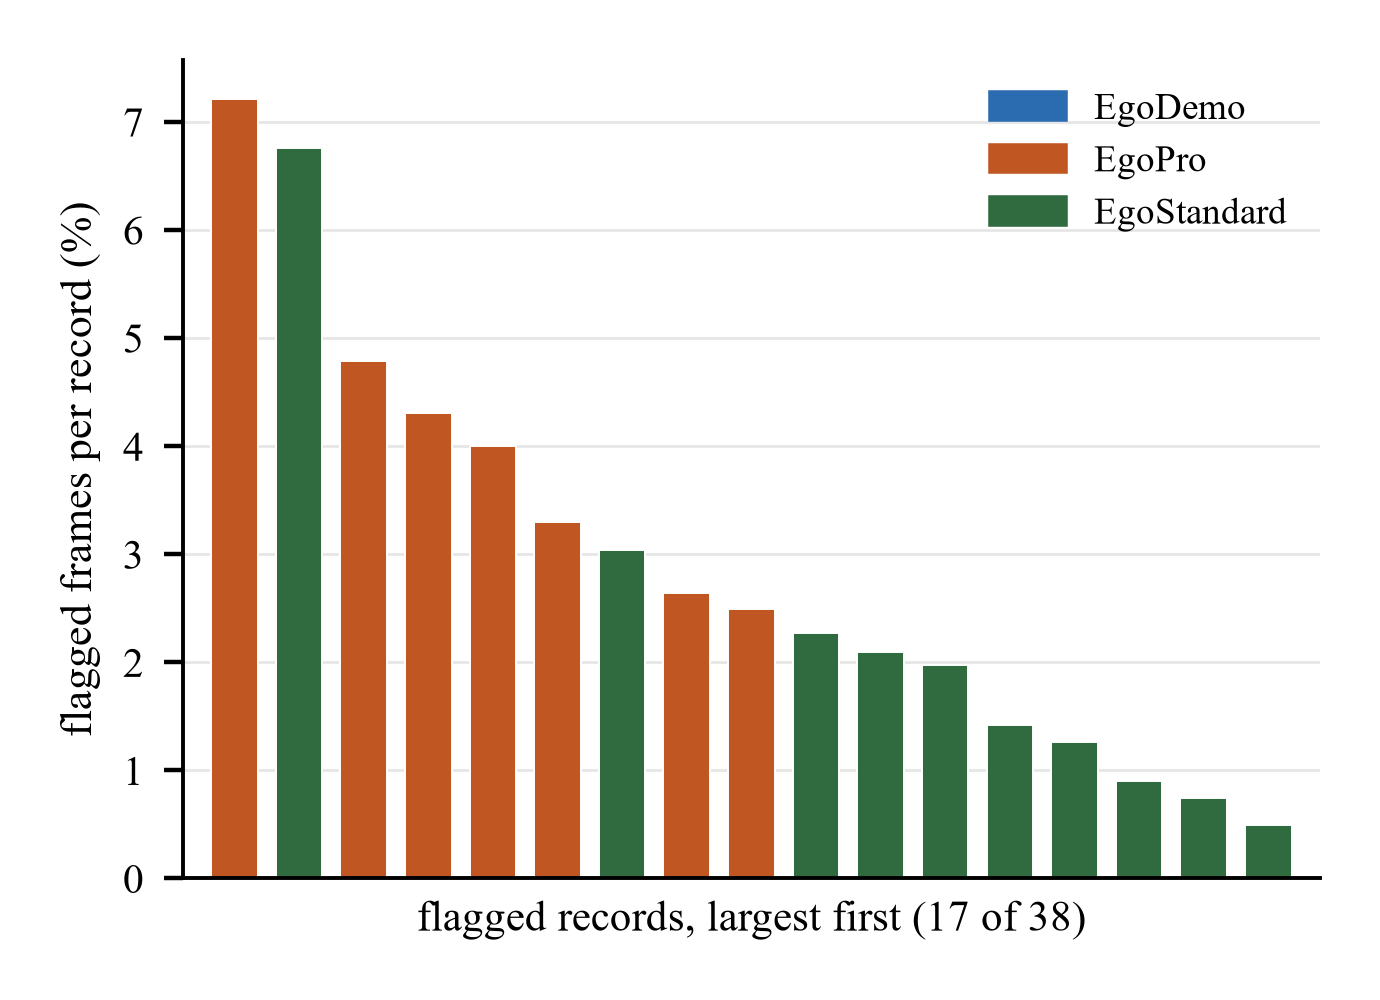
\includegraphics[width=0.47\linewidth]{figures/fig_n_badshare.png}}
\hfill
\subfigure[ARI gain of the learned decoder]{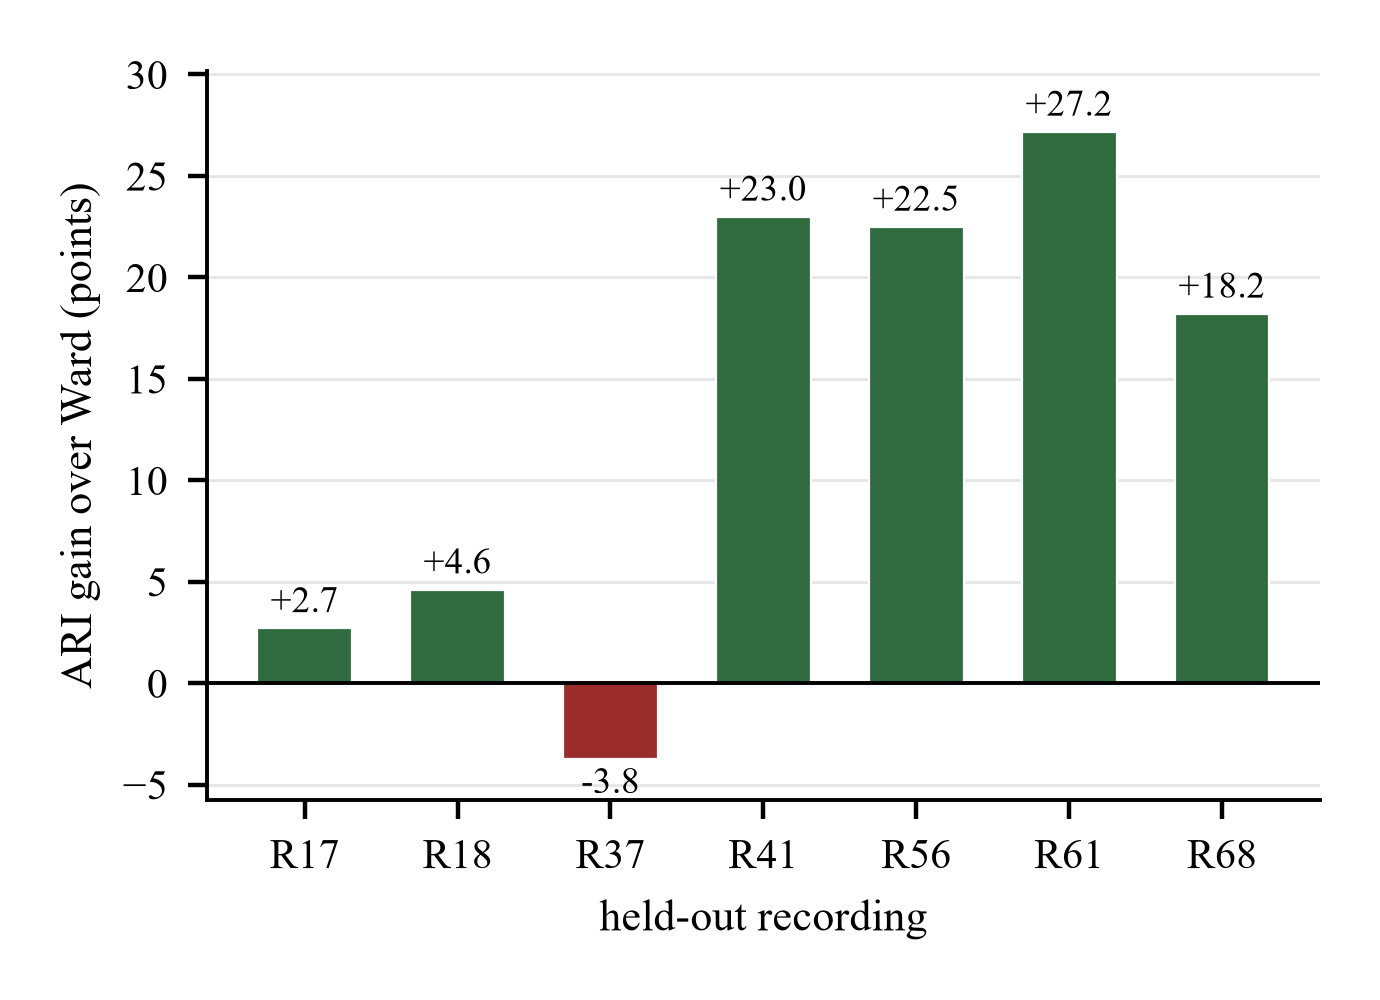
\includegraphics[width=0.47\linewidth]{figures/fig_n_arigain.png}}
\caption{Two views of the same evaluation records: the seventeen records that carry any flag
(left, ordered by share, out of the thirty-eight annotated records), and the per-record gain
of the learned boundary decoder over chain-constrained agglomeration (right), positive on six
of seven held-out records.}
\label{fig:twoviews}
\end{figure}
% numerals-ok: end


\section{Validation notes}
\label{app:valnotes}

% Validation notes moved from the body during the presentation pass.
% Every number is produced by the same slots as the body.
\subsection*{Validation notes moved from the body}

\noindent\textbf{Part I.} The split is by environment, so every test number here is a cross-environment number, and
the threshold sweep reports retention, recall and precision on one curve, which makes the
precision collapse at high thresholds a stated property, not a surprise. Stressing the
two test environments separately (Appendix~\ref{app:ablation}): \texttt{\slotPEnvOneName}
holds \slotPEnvOneN{} frames with \slotPEnvOnePos{} positives and \texttt{\slotPEnvTwoName}
\slotPEnvTwoN{} frames with \slotPEnvTwoPos{}, scoring \slotPEnvOneAUC{} and
\slotPEnvTwoAUC{}. The pre-declared mark was AUC above \slotPassAUC{} with average precision
above prevalence: the pooled split passes, the courier-station environment does not.

\noindent\textbf{Part II.} Validation has three legs. The predictors are compared on identical windows, so
the comparison is paired by construction. Coverage is checked against the nominal
level, and the pass mark is coverage of at least \slotConfLevel{}\% minus a
tolerance of five points. The crossover is checked against an independent probe
with different sampling, which agrees at the middle horizons and disagrees at the
shortest one; the two curves are reported separately and never merged. The economic
conclusion is re-run over a grid of cost coefficients, which is why
Section~\ref{sec:p2disc} quotes a range, not a single optimum. Conditional coverage at the
longest official prefix ranges from \slotPConCovMin{} to \slotPConCovMax{} across the
\slotPConCovNEnv{} test environments, against a marginal \slotPConCovMarginal{}; one
environment falls below $0.85$ (\slotPConCovBelow{} of \slotPConCovNEnv{}). The marginal
guarantee does not promise the former, and with one to three test records per environment a
per-environment conformal calibration cannot be estimated, so we report the spread as a
limitation instead of calibrating four radii.

\noindent\textbf{Part III.} The paired comparison is the primary evidence: every policy sees the same durations on the
same seed, so seed noise cancels. The interval against the reference excludes zero in both
informative cases, so the ordering is not seed luck. Against \textsc{risk}, the variant that
spends reviews, the interval
\slotPStochPairSTwoRiskFusionDiff{}$\pm$\slotPStochPairSTwoRiskFusionCI{} and
\slotPStochPairSThreeRiskFusionDiff{}$\pm$\slotPStochPairSThreeRiskFusionCI{} covers zero,
so paying for observations is not a gain this experiment can detect. The fused-predictor
variant is worse than the plain one in S\slotCaseTwo{} by
\slotPStochPairSTwoSlackFusionDiff{} and indistinguishable in S\slotCaseThree, a warning
about stacking models, not a result about scheduling.

Two secondary checks bound the claim. The first is the mapping, and Table~\ref{tab:maps} puts
it on the record: across the five published mappings the reference moves by
\slotPMapRefSpanSTwo{} points in S\slotCaseTwo{} and \slotPMapRefSpanSThree{} in
S\slotCaseThree, while the frozen rule moves by \slotPMapOursSpanSTwo{} and
\slotPMapOursSpanSThree{}. No scheduler-only change in this paper moves the rate by that much,
so the mapping stays in the paper as the dominant factor, and the gain of the rule is quoted
inside a mapping and never across one. It is not uniform: the mean paired gain is
\slotPMapGainMeanSTwo{} and \slotPMapGainMeanSThree{} points, the weakest cell gains
\slotPMapGainMinSTwo{} and \slotPMapGainMinSThree{}, and \slotPMapSatSTwo{} cell in
S\slotCaseTwo{} is saturated, where the reference already reaches the rule.


\end{appendices}

\end{document}
